%% fcup-thesis.tex -- document template for PhD theses at FCUP
%%
%% Copyright (c) 2015 João Faria <joao.faria@astro.up.pt>
%%
%% This work may be distributed and/or modified under the conditions of
%% the LaTeX Project Public License, either version 1.3c of this license
%% or (at your option) any later version.
%% The latest version of this license is in
%%     http://www.latex-project.org/lppl.txt
%% and version 1.3c or later is part of all distributions of LaTeX
%% version 2005/12/01 or later.
%%
%% This work has the LPPL maintenance status "maintained".
%%
%% The Current Maintainer of this work is
%% João Faria <joao.faria@astro.up.pt>.
%%
%% This work consists of the files listed in the accompanying README.

%% SUMMARY OF FEATURES:
%%
%% All environments, commands, and options provided by the `ut-thesis'
%% class will be described below, at the point where they should appear
%% in the document.  See the file `ut-thesis.cls' for more details.
%%
%% To explicitly set the pagestyle of any blank page inserted with
%% \cleardoublepage, use one of \clearemptydoublepage,
%% \clearplaindoublepage, \clearthesisdoublepage, or
%% \clearstandarddoublepage (to use the style currently in effect).
%%
%% For single-spaced quotes or quotations, use the `longquote' and
%% `longquotation' environments.


%%%%%%%%%%%%         PREAMBLE         %%%%%%%%%%%%

%%  - Default settings format a final copy (single-sided, normal
%%    margins, one-and-a-half-spaced with single-spaced notes).
%%  - For a rough copy (double-sided, normal margins, double-spaced,
%%    with the word "DRAFT" printed at each corner of every page), use
%%    the `draft' option.
%%  - The default global line spacing can be changed with one of the
%%    options `singlespaced', `onehalfspaced', or `doublespaced'.
%%  - Footnotes and marginal notes are all single-spaced by default, but
%%    can be made to have the same spacing as the rest of the document
%%    by using the option `standardspacednotes'.
%%  - The size of the margins can be changed with one of the options:
%%     . `narrowmargins' (1 1/4" left, 3/4" others),
%%     . `normalmargins' (1 1/4" left, 1" others),
%%     . `widemargins' (1 1/4" all),
%%     . `extrawidemargins' (1 1/2" all).
%%  - The pagestyle of "cleared" pages (empty pages inserted in
%%    two-sided documents to put the next page on the right-hand side)
%%    can be set with one of the options `cleardoublepagestyleempty',
%%    `cleardoublepagestyleplain', or `cleardoublepagestylestandard'.
%%  - Any other standard option for the `report' document arclass can be
%%    used to override the default or draft settings (such as `10pt',
%%    `11pt', `12pt'), and standard LaTeX packages can be used to
%%    further customize the layout and/or formatting of the document.

%% *** Add any desired options. ***
%PDF
%\documentclass[a4paper,narrowmargins,12pt,oneside,draft,onehalfspaced,singlespacednotes]{fcup-thesis}
%\documentclass[a4paper,narrowmargins,12pt,oneside,onehalfspaced,singlespacednotes]{fcup-thesis}
%Print
%\documentclass[draft,a4paper,narrowmargins,12pt,twoside,openright,onehalfspaced,singlespacednotes]{fcup-thesis}
\documentclass[a4paper,narrowmargins,12pt,twoside,openright,onehalfspaced,singlespacednotes]{fcup-thesis}

%% *** Add \usepackage declarations here. ***
%% The standard packages `geometry' and `setspace' are already loaded by
%% `ut-thesis' -- see their documentation for details of the features
%% they provide.  In particular, you may use the \geometry command here
%% to adjust the margins if none of the ut-thesis options are suitable
%% (see the `geometry' package for details).  You may also use the
%% \setstretch command to set the line spacing to a value other than
%% single, one-and-a-half, or double spaced (see the `setspace' package
%% for details).
% Overfull statements
\pretolerance=150
\setlength{\emergencystretch}{3em}
% Overfull end
\usepackage[english]{babel}
\usepackage{lipsum}
\usepackage[utf8]{inputenc}


%%% Additional useful packages
%%% ----------------------------------------------------------------
\usepackage{array}
\usepackage{amsmath}  
\usepackage{amssymb}
\usepackage{amsfonts}
\DeclareFontFamily{OT1}{pzc}{}
\DeclareFontShape{OT1}{pzc}{m}{it}{<-> s * [0.900] pzcmi7t}{}
\DeclareMathAlphabet{\mathpzc}{OT1}{pzc}{m}{it}
\usepackage{amsthm}      
\usepackage[ruled,algochapter]{algorithm2e}
\usepackage{algorithmic}
\usepackage{bm}
\usepackage[mathscr]{euscript}
\usepackage{graphicx}       
\usepackage{psfrag}         
\usepackage{fancyvrb}    
\usepackage{float}
\usepackage{ltablex}
\usepackage[square,sort,comma,numbers]{natbib}        
\usepackage{bbding}         
\usepackage{dcolumn}        
\usepackage{booktabs} 
\usepackage{multirow}
\usepackage{paralist}     
\usepackage{ifdraft}  
\usepackage{indentfirst}    
\usepackage[nottoc,notlof,notlot]{tocbibind}
\usepackage{url}
\usepackage{tabularx}
\usepackage{subcaption}
\usepackage[unicode]{hyperref}
\usepackage{xcolor}

\hypersetup{pdftitle=LiDAR obstacle detection and avoidance, 
            pdfauthor=Alojz Gomola,
            colorlinks=false,
            urlcolor=blue,
            pdfstartview=FitH,
            pdfpagemode=UseOutlines,
            pdfnewwindow,
            breaklinks
          }
\usepackage{array}
\newcolumntype{L}[1]{>{\raggedright\let\newline\\\arraybackslash\hspace{0pt}}m{#1}}
\newcolumntype{C}[1]{>{\centering\let\newline\\\arraybackslash\hspace{0pt}}m{#1}}
\newcolumntype{R}[1]{>{\raggedleft\let\newline\\\arraybackslash\hspace{0pt}}m{#1}}         
\newcolumntype{B}{X}
\newcolumntype{S}[1]{>{\hsize=#1\textwidth}X}

\newcommand{\FIGDIR}{./Pics}    %%% directory containing figures
\newcommand{\twolinecellr}[2][r]{%
  \begin{tabular}[#1]{@{}r@{}}#2\end{tabular}}
\newcommand{\secState}[1]{
	\ifdraft{(#1) }{}
}
\theoremstyle{plain}
\newtheorem{theorem}{Theorem}
\newtheorem{lemma}[theorem]{Lemma}
\newtheorem{proposition}[theorem]{Proposition}

\theoremstyle{plain}
\newtheorem{definition}{Definition}
\newtheorem{problem}{Problem}
\newtheorem{example}{Example}
\newtheorem{assumption}{Assumption}

\theoremstyle{remark}
\newtheorem*{corollary}{Corollary}
\newtheorem*{note}{Note}




\newenvironment{dokaz}{
  \par\medskip\noindent
  \textit{Proof}.
}{
\newline
\rightline{\SquareCastShadowBottomRight}
}

\newenvironment{constraints}[1]{
  \par\medskip\noindent
  \textit{Constraints #1} \\
}{
\newline
\rightline{\SquareCastShadowBottomRight}
}


%\bibliographystyle{plainnat}     %% Author (year) style
\bibliographystyle{unsrt}        %% [number] style
\setcitestyle{square}

% Section  3.7 Challenge list
\newif\ifproblemchallenge   %# Build block for problem challenges
\problemchallengetrue       %# Show comments

\newcommand{\R}{\mathbb{R}}
\newcommand{\N}{\mathbb{N}}

\DeclareMathOperator{\pr}{\textsf{P}}
\DeclareMathOperator{\E}{\textsf{E}\,}
\DeclareMathOperator{\var}{\textrm{var}}
\DeclareMathOperator{\sd}{\textrm{sd}}


\newcommand{\T}[1]{#1^\top}        

\newcommand{\goto}{\rightarrow}
\newcommand{\gotop}{\stackrel{P}{\longrightarrow}}
\newcommand{\maon}[1]{o(n^{#1})}
\newcommand{\abs}[1]{\left|{#1}\right|}
\newcommand{\dint}{\int_0^\tau\!\!\int_0^\tau}
\newcommand{\isqr}[1]{\frac{1}{\sqrt{#1}}}
\newcommand{\norm}[1]{\left\lVert#1\right\rVert}


\newcommand{\pulrad}[1]{\raisebox{1.5ex}[0pt]{#1}}
\newcommand{\mc}[1]{\multicolumn{1}{c}{#1}}
\newcommand{\TBD}[1]{\color{red}\emph{--TBD:}#1\color{black}}

%%%%%%%%%%%%%%%%%%%%%%%%%%%%%%%%%%%%%%%%%%%%%%%%%%%%%%%%%%%%%%%%%%%%%%%%
%%                                                                    %%
%%                   ***   I M P O R T A N T   ***                    %%
%%                                                                    %%
%%  Fill in the following fields with the required information:       %%
%%   - \degree{...}       name of the degree obtained                 %%
%%   - \department{...}   name of the graduate department             %%
%%   - \gradyear{...}     year of graduation                          %%
%%   - \author{...}       name of the author                          %%
%%   - \title{...}        title of the thesis                         %%
%%%%%%%%%%%%%%%%%%%%%%%%%%%%%%%%%%%%%%%%%%%%%%%%%%%%%%%%%%%%%%%%%%%%%%%%

%% *** Change this example to appropriate values. ***
\degree{Doctor of Philosophy}
\department{Departamento de Matem\'{a}tica}
\gradyear{2019}
\author{Alojz Gomola}
\title{Obstacle Avoidance Framework based on Reach Sets}

%% *** NOTE ***
%% Put here all other formatting commands that belong in the preamble.
%% In particular, you should put all of your \newcommand's,
%% \newenvironment's, \newtheorem's, etc. (in other words, all the
%% global definitions that you will need throughout your thesis) in a
%% separate file and use "\input{filename}" to input it here.


%% *** Adjust the following settings as desired. ***

%% List only down to subsections in the table of contents;
%% 0=chapter, 1=section, 2=subsection, 3=subsubsection, etc.
\setcounter{tocdepth}{3}

%% Make each page fill up the entire page.
\flushbottom


%%%%%%%%%%%%      MAIN  DOCUMENT      %%%%%%%%%%%%

\begin{document}


%%%%%%%%%%%%%%%%%%%%%%%%%%%%%%%%%%%%%%%%%%%%%%%%%%%%%%%%%%%%%%%%%%%%%%%%
%%  Put your Chapters here; the easiest way to do this is to keep     %%
%%  each chapter in a separate file and `\include' all the files.     %%
%%  Each chapter file should start with "\chapter{ChapterName}".      %%
%%  Note that using `\include' instead of `\input' will make each     %%
%%  chapter start on a new page, and allow you to format only parts   %%
%%  of your thesis at a time by using `\includeonly'.                 %%
%%%%%%%%%%%%%%%%%%%%%%%%%%%%%%%%%%%%%%%%%%%%%%%%%%%%%%%%%%%%%%%%%%%%%%%%

%% *** Include chapter files here. ***

\setcounter{chapter}{7}
\setcounter{section}{3}

    \cleardoublepage
\section{\secState{D}Cooperative Test Cases}\label{s:cooperativeTestCases}
    
    \noindent The \emph{main goal} of this section is to show the operational capabilities of \emph{approach} under \emph{UTM supervision}. The minimal UTM functionality set (sec. \ref{sec:UASTrafficManagement}) has been implemented, including \emph{position notifications mechanism, collision case calculation, resolution enforcement} components. 
    
    Test cases covers \emph{well clear breach prevention}, \emph{situation based avoidance}, and \emph{rules of the air enforcement}. 
    
    Coverage of \emph{near miss situations}, \emph{clash incidents} is given implicitly by \emph{safety} and \emph{body} margins (tab. \ref{tab:controlledAirspaceViolations}).
    
    \begin{enumerate}
        \item \emph{Rule based converging} (sec. \ref{s:testRuleConverging}) covers \emph{well clear breach} and \emph{converging rule of the air}, showing determinism and \emph{UTM resolution execution}.
        
        \item \emph{Rule based head on} (sec. \ref{s:testRuleHeadOn}) covers \emph{well clear breach} and \emph{head on rule of the air}, showing determinism and \emph{UTM resolution execution}.
        
        \item \emph{Rule based mixed head on with converging} (sec. \ref{s:testRuleMixed}) covers \emph{well clear breach} and \emph{head on and converging rules of the air}. The main focus is on \emph{virtual roundabout} concept, when multiple collision cases are clustered into one avoidance maneuver. 
        
        \item \emph{Rule based overtake} (sec. \ref{s:testRuleOvertake}) covers \emph{well clear breach} during \emph{overtake} by faster UAS.
    \end{enumerate}


    	\subsection{Rule based Converging}\label{s:testRuleConverging}

\paragraph{Scenario:} Two \emph{UAS} are approaching an \emph{airway intersection} at \emph{same time} in \emph{controlled airspace} (over 500 feet Above the Ground Level). The mutual position of \emph{UAS} can be classified as \emph{Side approach}. Following \emph{collision hazards} are present:

\begin{enumerate}
    \item \emph{Active Converging Collision Hazard} -  There is an \emph{UAS} approaching from the \emph{right side}, which give him \emph{Right of the Way} and invokes need to actively avoid \emph{Intruder}.

	\item \emph{Passive Converging Collision Hazard} - There is an \emph{UAS} approaching from the \emph{left side}, which gave us \emph{Right of the Way} and imposes an obligation of \emph{active avoidance} on other \emph{UAS}.
	
\end{enumerate}


\noindent\emph{Collision Hazards} must be addressed by \emph{UTM} service in the following manner:


\begin{enumerate}
	\item \emph{Each UAS} in particular \emph{Controlled Space} periodically sends synchronized \emph{Position Notification} messages (tab. \ref{tab:positionNotification}). 
	
	\item \emph{UTM} service receives \emph{Position Notifications} and manages \emph{Collision Case} (tab. \ref{tab:collisionCase}) in \emph{Controlled Space}. 
	
	\item \emph{UTM} detects \emph{Converging Collision Case} with \emph{Collision Point} in  vicinity.
	
	\item \emph{UTM} service Sends \emph{Mandate} to UAS without \emph{Right of the Way} and implements \emph{Normative Directive} on all \emph{UAS} in area.
\end{enumerate}


\noindent\emph{Mission parameters} for both UAS systems are defined in (tab. \ref{tab:missionSetupRuleBasedConvergingScenario}).

\begin{table}[H]
    \centering
    \begin{tabular}{c||c|c||c}
        \multirow{2}{*}{UAS} &\multicolumn{2}{c||}{Position} & \multirow{2}{*}{$\mathscr{WP}_1$} \\\cline{2-3}
          & $[x,y,z]$           & $[\theta,\varpi,\psi]$           & \\\hline\hline
        1 & $[0,20,0]^T $       & $[0^\circ,0^\circ,0^\circ]^T$    & $[40,20,0]^T$\\\hline 
        2 & $[20,0,0]^T $       & $[0^\circ,0^\circ,90^\circ]^T$    & $[20,40,0]^T$\\
    \end{tabular}
    \caption{Mission setup for \emph{Rule based converging} scenario.}
    \label{tab:missionSetupRuleBasedConvergingScenario}
\end{table}


\paragraph{Assumptions:} Following assumptions are valid for this test:

\begin{enumerate}
	\item \emph{Controlled Airspace Airworthiness} - UAS system is equipped with necessary controlled airspace equipment like ADS-B In/Out, Radar, Transponder, etc. Moreover airworthy \emph{UAS} has capability to precisely follow \emph{UTM directives} (max. 5 $\%$ deviation).
	
	\item \emph{C2 (Command \& control) Link Established} - necessary for (UAS $\leftrightarrow$ UAS) and (UAS $\leftrightarrow$ UTM) communication. If \emph{C2} link is lost the \emph{UAS} will enter into \emph{Emergency avoidance mode}.
	
	\item \emph{Decision frame synchronization with UTM} - necessary in discrete C2 environment otherwise \emph{safety margins} needs to be \emph{bloated}.
	
	\item \emph{Both UAS have identical cruising speed} - simplification impacting \emph{UTM} service implementation. \emph{Obstacle Avoidance Framework} can comprehend various intruders speed, with proper \emph{UAS} directives.
\end{enumerate}

\paragraph{Main Goal:} Show possibility of \emph{Converging situation resolution} with \emph{forced safety margin} by \emph{UAS Traffic Management} system.  The \emph{Obstacle Avoidance Framework based on Reach Sets} is used as \emph{Navigation Module}.

\paragraph{Acceptance  Criteria:} Following criteria must be met:

\begin{enumerate}
	\item \emph{Well Clear Condition valid for both UAS} - Both \emph{UAS} must have \emph{minimal required distance} from \emph{other UAS} for all \emph{Converging Maneuver} enforcement time.
	
	\item \emph{Fulfillment of UTM Directives} - Both UAS must stay in \emph{Navigation mode} for all \emph{Converging Maneuver} enforcement time. \emph{UAS without Right Of the Way} must stay away for necessary time, before returning to \emph{Original Navigation waypoint $\mathscr{WP}_1$} following.
\end{enumerate}


\paragraph{Testing Setup:} The \emph{standard test setup} for each UAS defined in (tab. \ref{tab:testMovementOrientations}, \ref{tab:testUASBasicParameters}, \ref{tab:testNavigationGridBasic}, \ref{tab:testAvoidanceGridBasic}, \ref{tab:testUASColoring}) is used with following parameter override:
\begin{enumerate}
	\item \emph{Navigation grid - type} - \emph{ACAS-like} with enabled \emph{Horizontal maneuvers}
\end{enumerate}

This \emph{configuration} is based on assumption that every UAS is in \emph{controlled airspace} in \emph{FL450} (flight level 45000 feet Above Sea Level), without permission for \emph{climb or descent maneuver}. \emph{Rule engine} is initialized in standard \emph{Rules of the air} configuration (fig. \ref{fig:RuleEngineInstanceLevels}).

There is \emph{UTM} service for given \emph{airspace cluster} calculating \emph{collision cases} (tab. \ref{tab:collisionCase}) based on incoming \emph{UAS position notifications} (tab. \ref{tab:positionNotification}).

\paragraph{Simulation Run:} Notable moments from \emph{simulation run} (fig. \ref{fig:testCaseRuleBasedConverging}) are following:

\begin{enumerate}
    \item \emph{Collision Case creation} (fig. \ref{fig:ruleBasedConvergingCollisionCaseCreation}) following events happens in this step:
    \begin{enumerate}[a.]
        \item Two \emph{UAS} are approaching  \emph{airway intersection}: UAS 1 (blue) from left and UAS 2 (cyan) from bottom.
        
        \item They are going to \emph{collide} at point $\mathscr{C}=[20,20,0]^T$ of \emph{Flight Level} (elevation is 45, 000 feet Above Mean Seal Level).
        
        \item UTM service notices future \emph{Collision Situation} and creates \emph{Collision Case}.
        
        \item \emph{Converging Directive} for 8 m from \emph{Collision point} is issued for UAS 1 (blue), because UAS 2 (cyan) has \emph{Right Of the Way}.
        
        \item \emph{Keep Velocity/Heading Directive} is issued for UAS 2 (cyan) to ensure avoidance maneuver success.
        
        \item UAS 1 (blue) corrects its heading according to \emph{UTM} directive.
        
        \item UAS 2 (cyan) stays on claimed course and if its necessary adjust its speed.
        
    \end{enumerate}
    
    \item \emph{Well clear before} (fig. \ref{fig:ruleBasedConvergingWellClearBefore}) UAS 1 (blue) checks the \emph{Collision Point} distance and keeps safe distance given by safety margin. UAS 2 (cyan) checks if there is no intruder in \emph{Avoidance Grid} and if not, stays in \emph{Navigation Mode}.
    
    \item \emph{Well clear after} (fig. \ref{fig:ruleBasedConvergingWellClearAfter}) UAS 2 (cyan) is \emph{after Collision Point}, it can start negotiations of new speed and heading with UTM. UAS 1 (blue) is still enforced to follow \emph{Converging Maneuver} directive, until the outer boundary of \emph{Collision Zone} is reached.
    
    \item \emph{Waypoints reach} (fig. \ref{fig:ruleBasedConvergingWaypointsReach})  UAS 1 (blue) leaves outer boundary of \emph{Collision zone}. Leaving \emph{Converging Maneuver Directive}. UTM closes \emph{Collision Case}.
\end{enumerate}


\begin{figure}[H]
    \centering
    \begin{subfigure}{0.48\textwidth}
    	\centering
        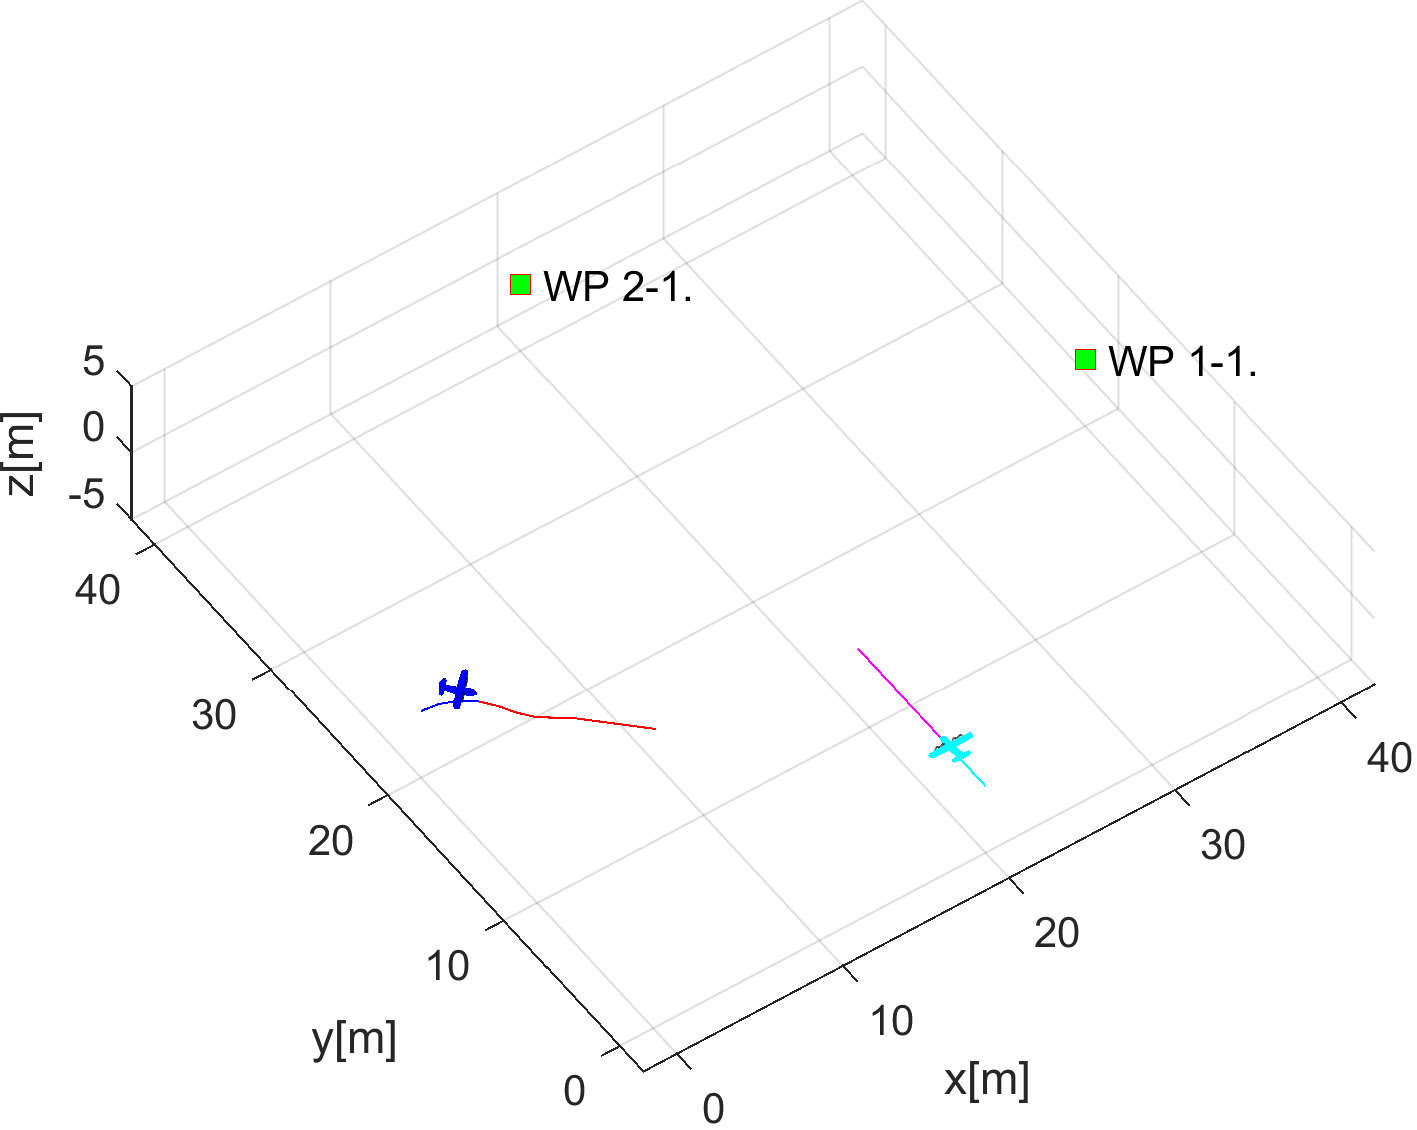
\includegraphics[width=0.9\linewidth]{\FIGDIR/NS048UtmCooperativeConverging00003}
        \caption{Collision case creation.}
        \label{fig:ruleBasedConvergingCollisionCaseCreation}
    \end{subfigure}
    \begin{subfigure}{0.48\textwidth}
    	\centering
        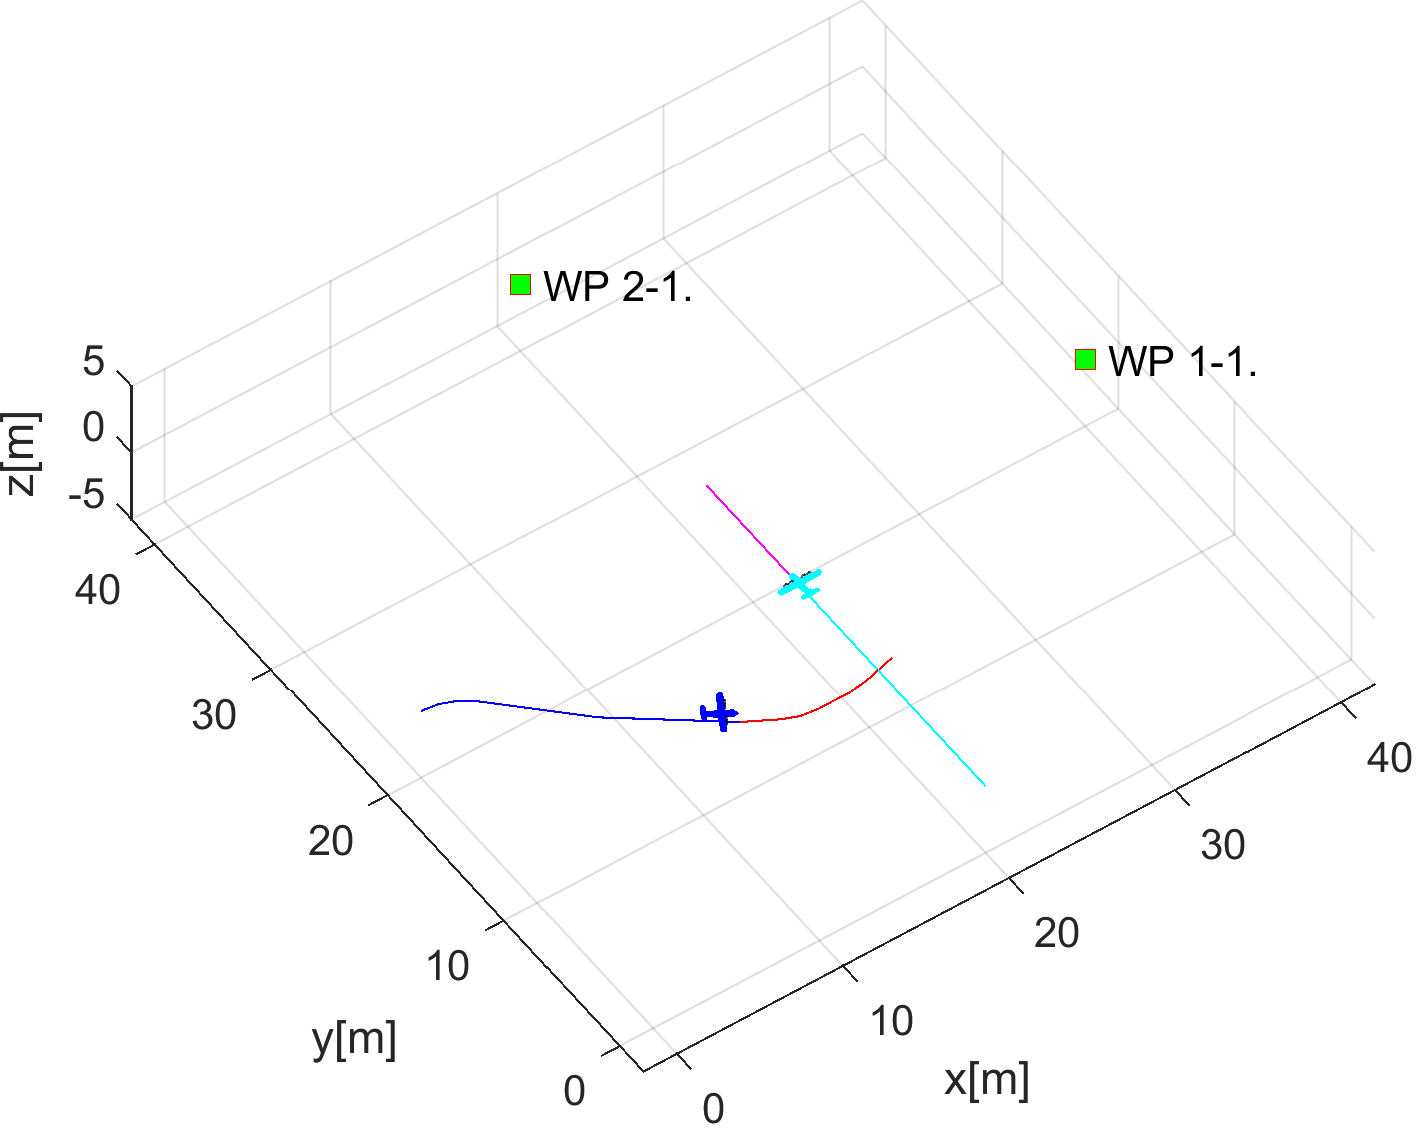
\includegraphics[width=0.9\linewidth]{\FIGDIR/NS049UtmCooperativeConverging00016} 
        \caption{Well clear before.}
        \label{fig:ruleBasedConvergingWellClearBefore}
    \end{subfigure}
    \\
    \begin{subfigure}{0.48\textwidth}
    	\centering
        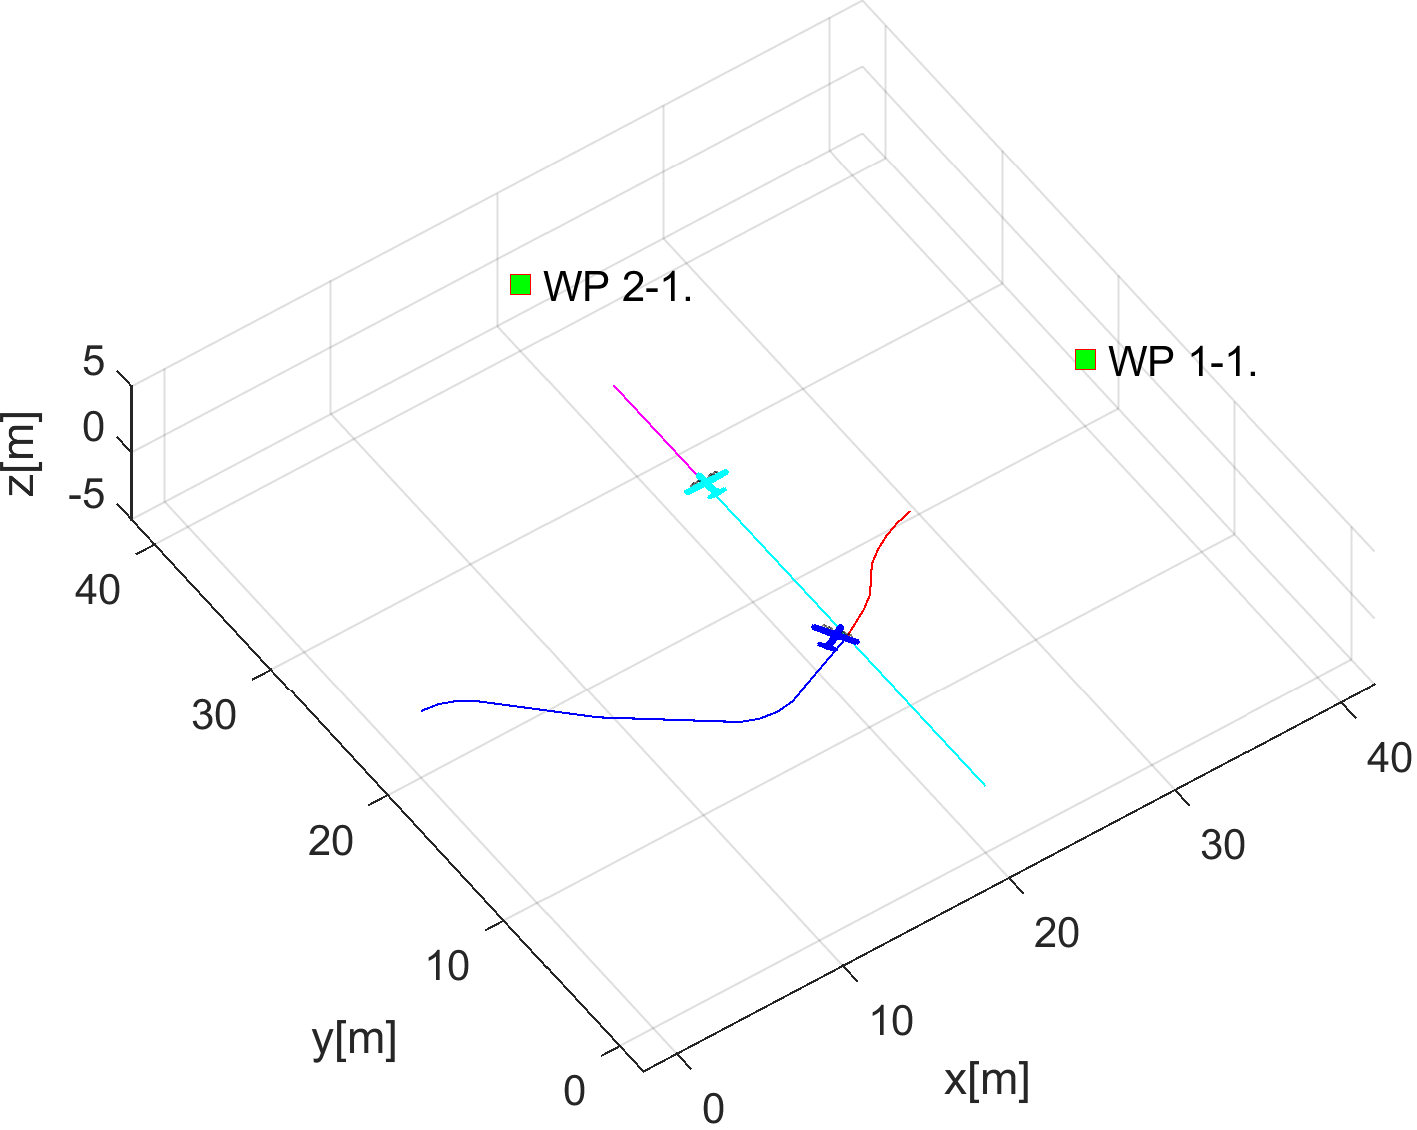
\includegraphics[width=0.9\linewidth]{\FIGDIR/NS050UtmCooperativeConverging00024} 
        \caption{Well clear after.}
        \label{fig:ruleBasedConvergingWellClearAfter}
    \end{subfigure}
    \begin{subfigure}{0.48\textwidth}
    	\centering
        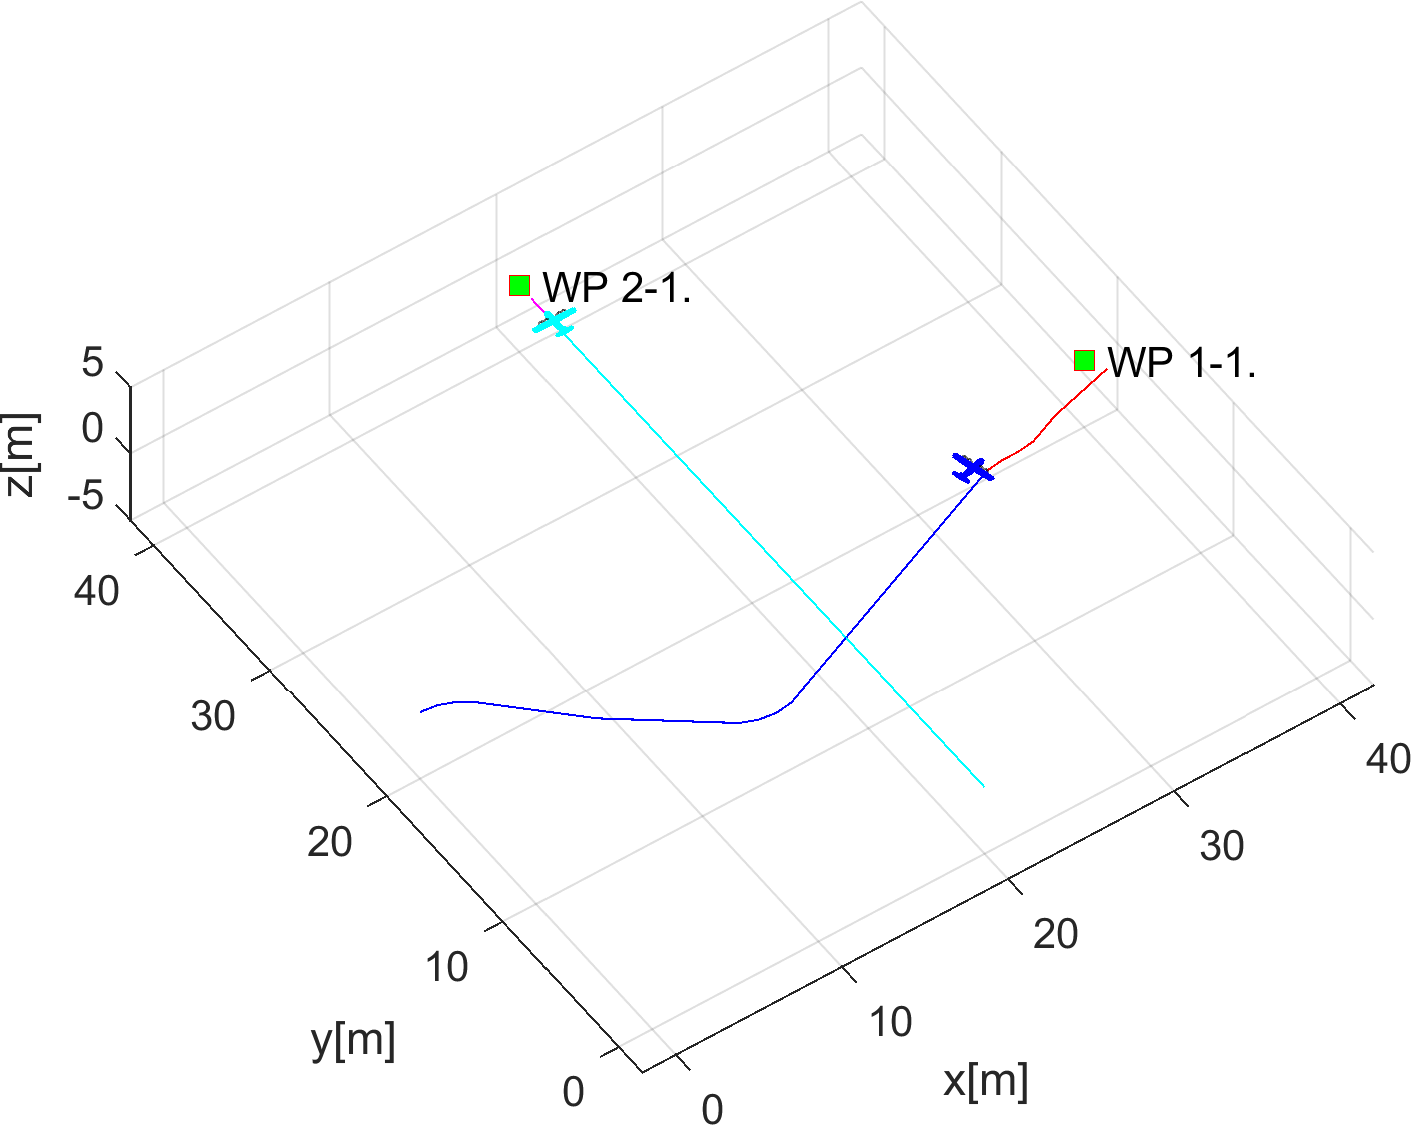
\includegraphics[width=0.9\linewidth]{\FIGDIR/NS051UtmCooperativeConverging00037} 
        \caption{Waypoints reach.}
        \label{fig:ruleBasedConvergingWaypointsReach}
    \end{subfigure}
    \caption{Test scenario for \emph{Rule based converging}. }
    \label{fig:testCaseRuleBasedConverging}
\end{figure}


\paragraph{Collision Case Calculation:} For test scenario in (fig. \ref{fig:testCaseRuleBasedConverging}) where UAS 1 (blue) is converging to avoid UAS 2 (cyan) the \emph{Collision Case} (tab. \ref{tab:collisionCasesRuleBasedConverging}) have been calculated. 

The \emph{Collision point} is at $[20,20,0]$ in \emph{Flight Level} $FL450$ coordinate frame.

The \emph{angle of approach} was evaluated as $90^{\circ}$ which indicates \emph{converging maneuver} in range $70^{\circ} \le angle Of Approach < 130^{\circ}$.

The \emph{mutual position} of UAS 1 (blue) and UAS 2(cyan) is giving the roles: \emph{Right Of the Way} for UAS 2 (cyan) and \emph{Converging} for UAS 1 (blue).

The \emph{safety margin} for \emph{Well Clear} was determined as $3m$ for UAS 1 and $5 m$ for UAS 2. (Note: Well Clear Margin is usually much greater than Near Miss margin). The \emph{Combined Case} margin which was enforced was $8 m$. The mutual distance can not go below this threshold. 


\begin{table}[H]
    \centering
    \begin{tabular}{c|c|c|c|c|c||c|c}
        \multicolumn{6}{c||}{Collision Case}& \multicolumn{2}{c}{Margins} \\ \hline
        id  & UAS & role & \begin{tabular}[c]{@{}c@{}}collision\\ point\end{tabular} & \begin{tabular}[c]{@{}c@{}}angle of\\ approach\end{tabular} & type&  safety  & case  \\ \hline\hline
        % Case 1-2
        \multirow{2}{*}{1-2} & 1   & Converging & \multirow{2}{*}{$[20,20,0]^T$} & \multirow{2}{*}{$90^\circ$} & \multirow{2}{*}{Converging} & 3 & \multirow{2}{*}{8} \\ \cline{2-3} \cline{7-7} & 2   & Right o. W. & & & & 5 & 
    \end{tabular}
    \caption{Collision case for \emph{Rule-based converging} scenario.}
    \label{tab:collisionCasesRuleBasedConverging}
\end{table}


\paragraph{Distance to Safety Margin Evolution:} The safety margin values (well clear) (fig. \ref{fig:testCaseRuleBasedConvergingAvoidancePerformance}) in controlled airspace are much greater than in non-controlled airspace (near miss) (fig. \ref{fig:testCaseEmergencyConvergingAvoidancePerformance}) 

The enforced rule was (rule \ref{tab:ruleConvergingManuever}) with parameters: Collision Point $[20,20,0]^T$ and \emph{Safety Margin} $8$ $m$ as given by Collision Case (tab. \ref{tab:collisionCasesRuleBasedConverging}).

The mutual \emph{UAS distance} (blue line) does not go over \emph{Safety Margin} (red line), which means UAS 1 well clear margin of $3$ $m$ and UAS 2 well clear margin of $5$ $m$ are not broken (fig. \ref{fig:testCaseRuleBasedConvergingAvoidancePerformance}).

\begin{figure}[H]
    \centering
    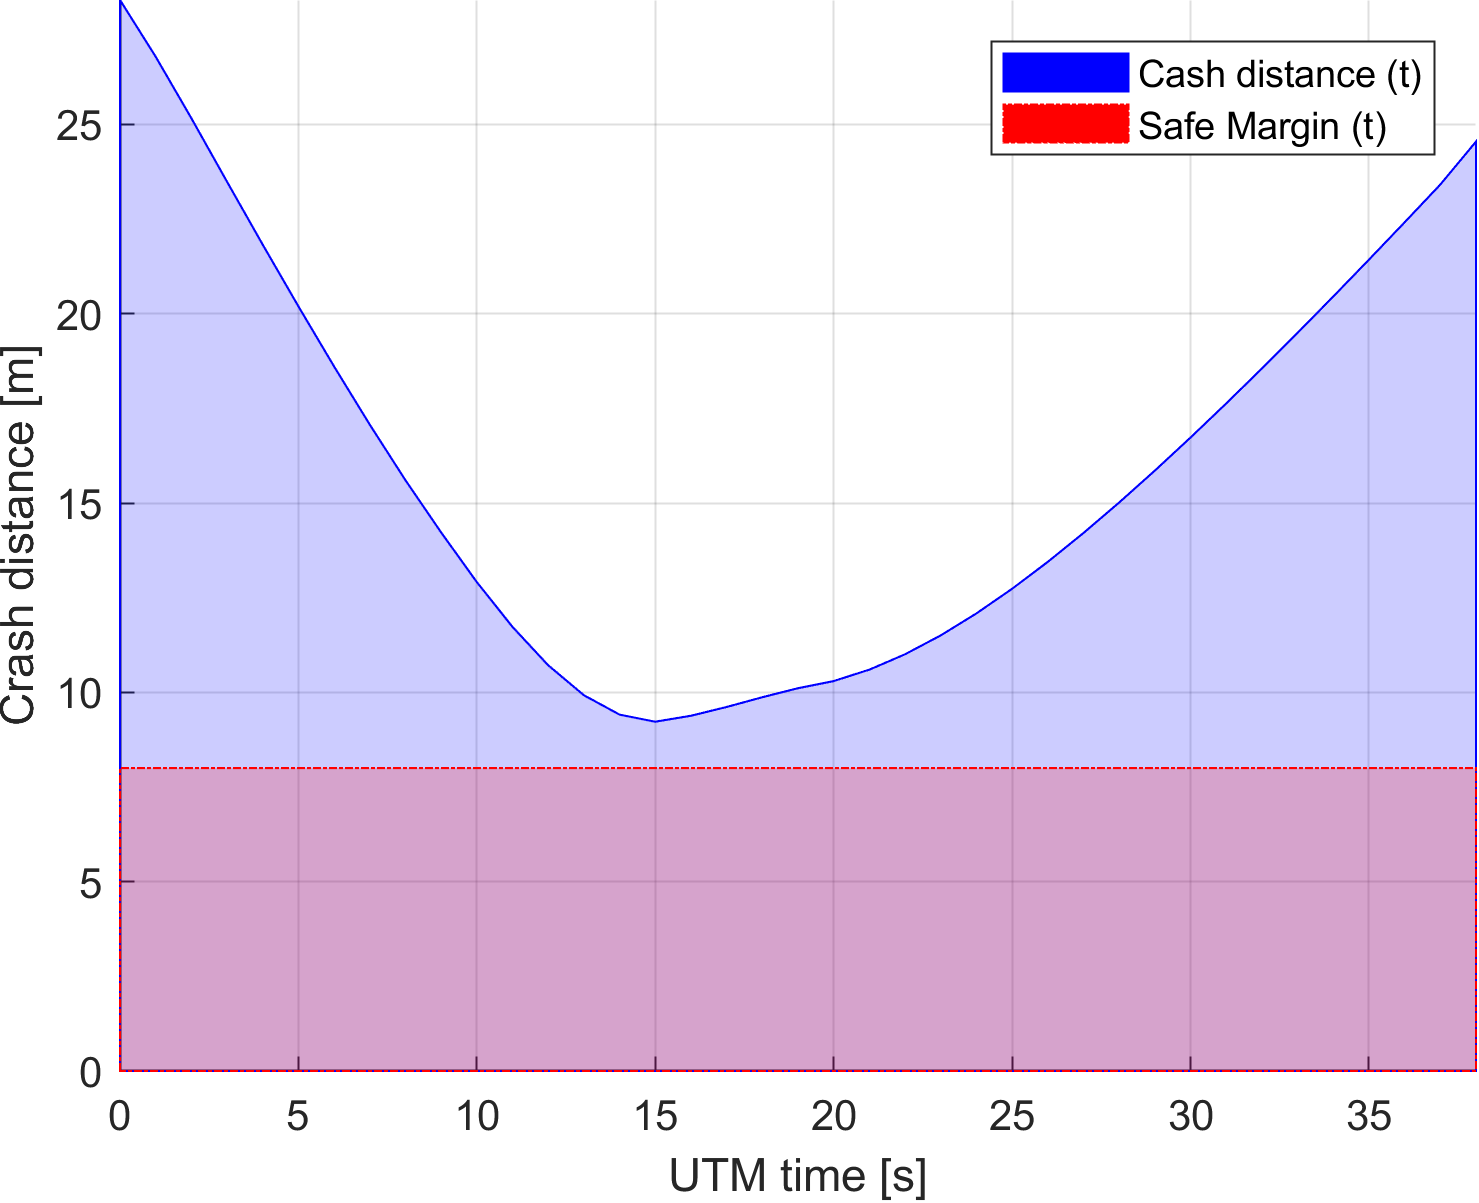
\includegraphics[width=0.55\linewidth]{\FIGDIR/NS052UtmCooperativeConvergingPerformance} 
    \caption{Distance to safety margin evolution for \emph{rule based converging scenario}.}
    \label{fig:testCaseRuleBasedConvergingAvoidancePerformance}
\end{figure}


\paragraph{Distance to Safety Margin Peaks:} \emph{Distance to safety margin peaks} (tab. \ref{tab:testCaseRuleBasedConvergingSafetyMarginDistances}) represent the proximity on UAS mutual distance to \emph{breach of well clear condition} (safety margin). The \emph{breach of well clear condition} was not achieved. The \emph{minimal distance to safety margin} was $1.2240$ $m$. The \emph{maximal distance to safety margin} was $20.2843$ $m$ which represents distance in time of \emph{Collision Case Creation}.

\begin{table}[H]
    \centering
    \begin{tabular}{c||c|c|c}
        \multirow{2}{*}{UAS:} & \multicolumn{3}{c}{Distance to Safety Margin} \\ \cline{2-4} 
                  & min          & max         & breach         \\ \hline\hline
            1-2   & 1.2240       & 20.2843     & false          \\ 
    \end{tabular}
    \caption{Distance to safety margin peaks for \emph{Rule based converging scenario}.}
    \label{tab:testCaseRuleBasedConvergingSafetyMarginDistances}
\end{table}

\paragraph{Path Tracking Performance:} \emph{Path tracking} is displayed in (fig. \ref{fig:ruleBasedConvergingTrajectoryTrackingPerformance}). The \emph{UAS} trajectory is divined into \emph{X, Y, Z axis tracking over UTM Time}. The \emph{Reference Trajectory} (green dashed line) interconnect starting position of UAS (green square marked S) an goal waypoint (green square marked 1). The \emph{Executed Trajectory} (blue solid line) reflects real UAS trajectory. 

\begin{enumerate}
    \item UAS 1. (fig, \ref{fig:ruleBasedConvergingUAS1PathTracking}) do steady right side \emph{converging maneuver} (y-axis).
    
    \item UAS 2. (fig. \ref{fig:ruleBasedCovnergingUAS2PathTracking}) follows the reference trajectory precisely, because it has \emph{Right Of the Way}.
\end{enumerate}

\begin{figure}[H]
    \centering
    \begin{subfigure}{0.48\textwidth}
    	\centering
        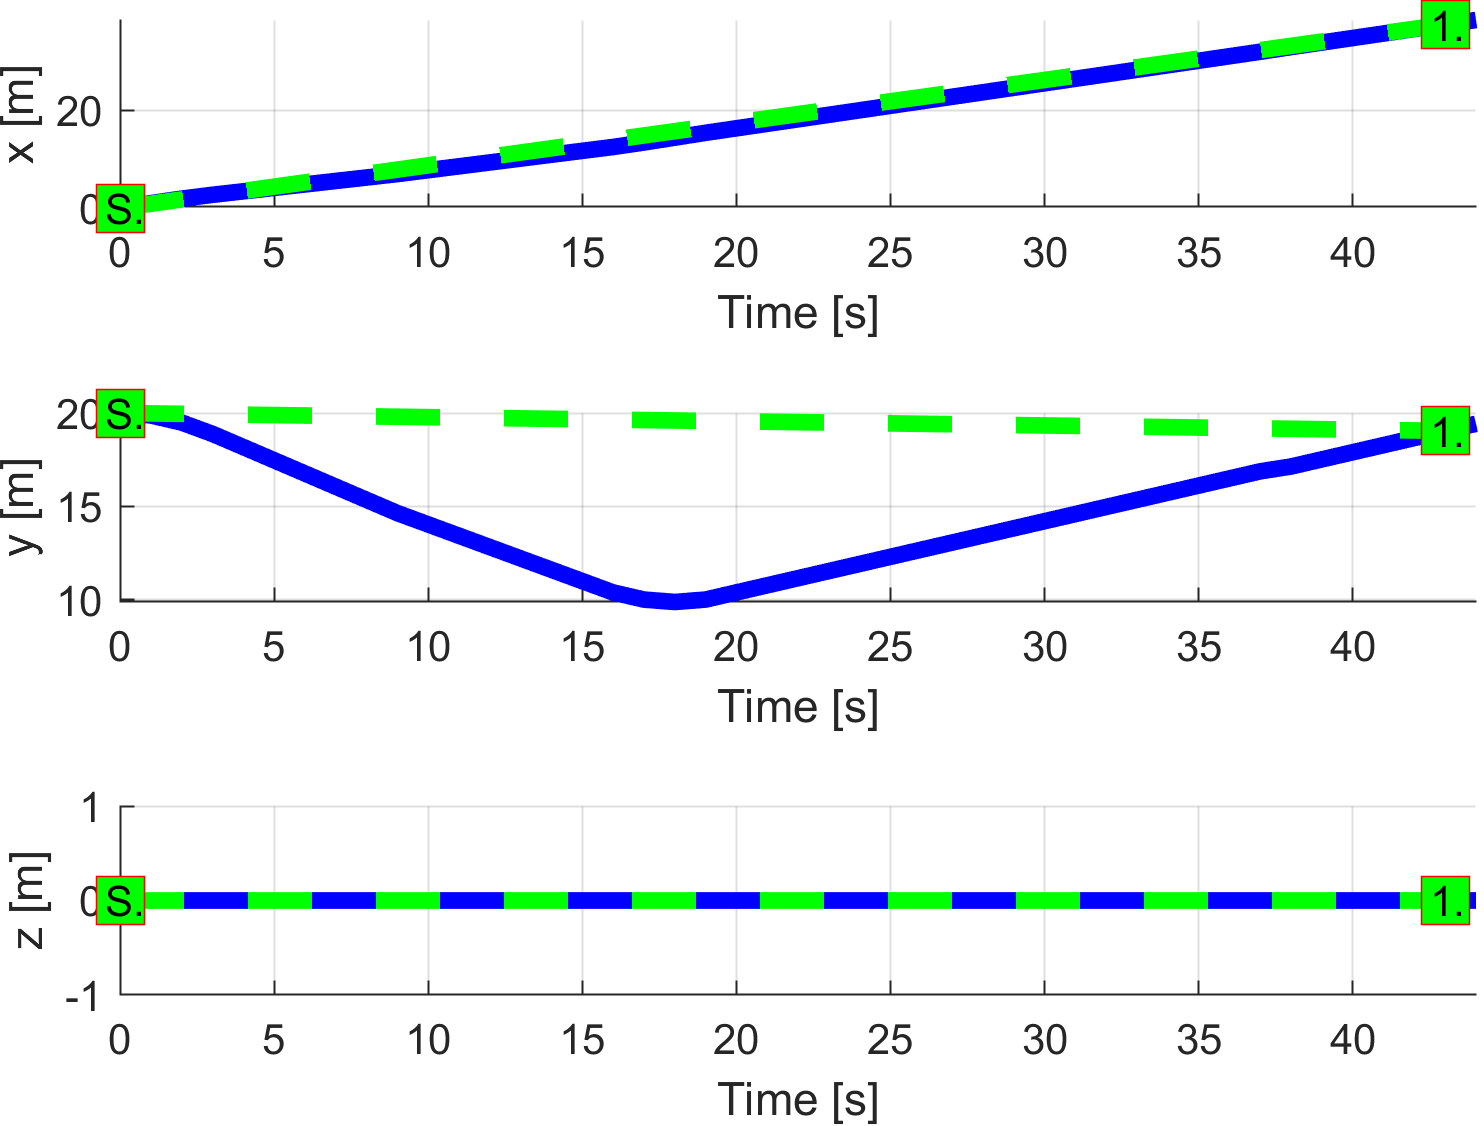
\includegraphics[width=0.9\linewidth]{\FIGDIR/NS053UtmCooperativeConvergingUAV1PathFollowing}
        \caption{UAS 1.}
        \label{fig:ruleBasedConvergingUAS1PathTracking}
    \end{subfigure}
    \begin{subfigure}{0.48\textwidth}
    	\centering
        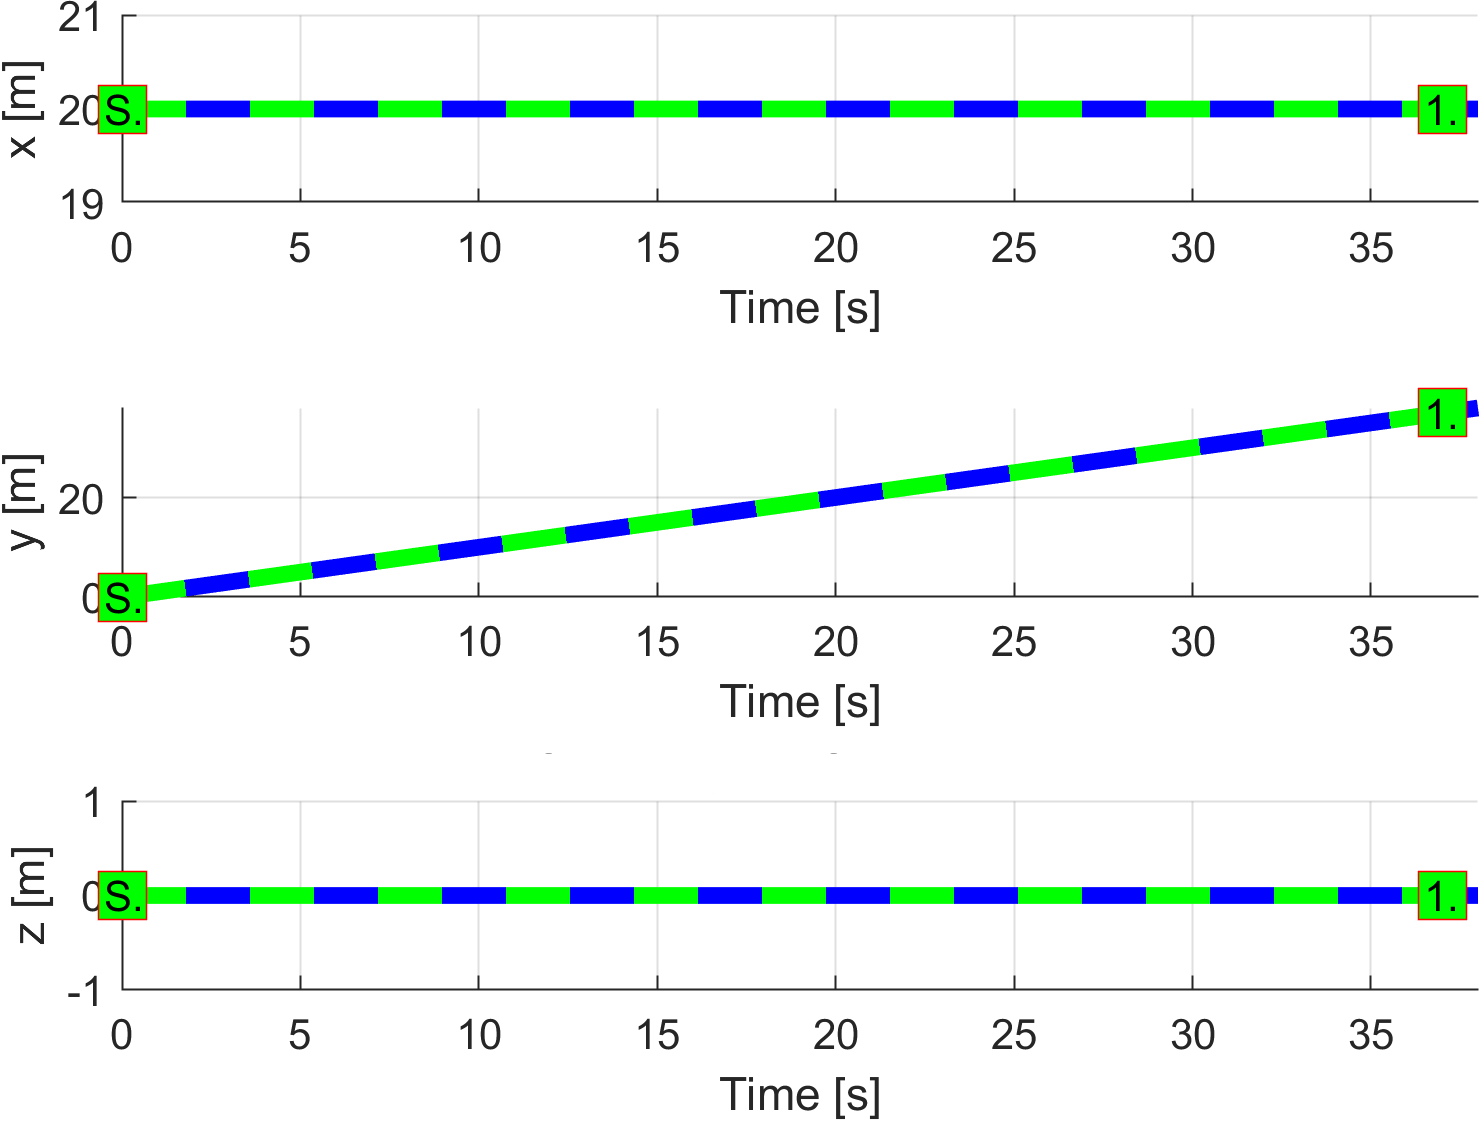
\includegraphics[width=0.9\linewidth]{\FIGDIR/NS054UtmCooperativeConvergingUAV2PathFollowing} 
        \caption{UAS 2.}
        \label{fig:ruleBasedCovnergingUAS2PathTracking}
    \end{subfigure}
    \caption{\emph{Trajectory tracking} for \emph{Rule based converging} test case. }
    \label{fig:ruleBasedConvergingTrajectoryTrackingPerformance}
\end{figure}

\paragraph{Path Tracking Deviations:} Deviations (tab. \ref{tab:pathTrackingParametersForRuleBasedConverging}) are in \emph{expected ranges}, considering the \emph{mission plans} (tab. \ref{tab:missionSetupRuleBasedConvergingScenario}) and \emph{Collision Case} safety margin of $8 m$.

The minimal deviation distance was expected at value of \emph{safety margin} ($8 m$). The maximal deviation was $10.22m$ which is acceptable due the space discretization, UAS dynamic, and, \emph{dynamic decision time}.

\begin{table}[H]
    \centering
    \begin{tabular}{c||c|c}
        \multirow{2}{*}{Param.} & UAS 1     & UAS 2              \\\cline{2-3}
                        & $\mathscr{WP}_1$  & $\mathscr{WP}_1$   \\\hline\hline
          $\max |x|$    & 0                 & 0                  \\\hline
          $\max |y|$    & 10.22             & 0                  \\\hline
          $\max |z|$    & 0                 & 0                  \\\hline
          $\max dist.$  & 10.22             & 0                  \\
    \end{tabular}
    \caption{Path tracking properties for \emph{Rule based converging} scenario.}
    \label{tab:pathTrackingParametersForRuleBasedConverging}
\end{table}

\paragraph{Computation Load:} The \emph{computation load} for \emph{scenario} (fig.\ref{fig:ruleBasedCConvergingComputationTime}) shows used time (y-axis) over decision frame (x-axis).

The \emph{computation time} is slightly increased for avoiding UAS 1 during avoidance. The initial increase of computation time UAS 2 is caused by UTM communication demand.

\begin{figure}[H]
    \centering
    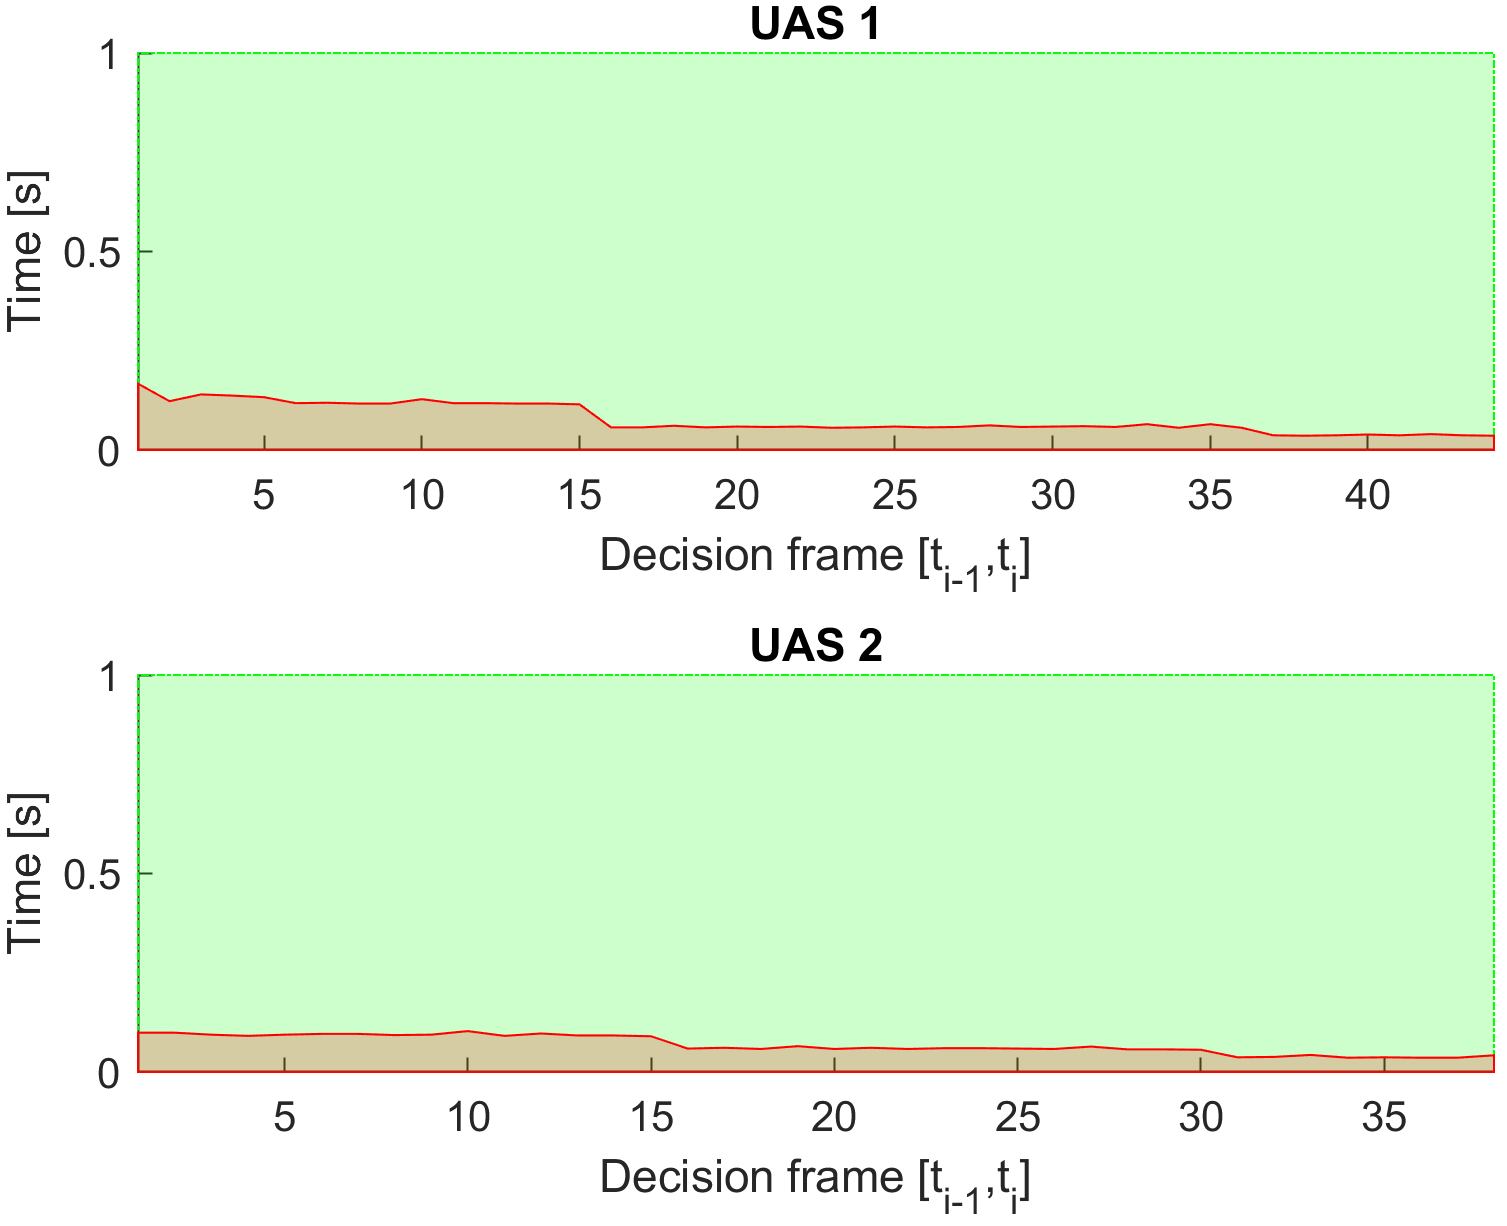
\includegraphics[width=0.65\linewidth]{\FIGDIR/NS099RuleBasedCConvergingComputationTime} 
    \caption{Computation time for \emph{Rule-based converging} scenario.}
    \label{fig:ruleBasedCConvergingComputationTime}
\end{figure}
    	\subsection{Rule based Head on}\label{s:testRuleHeadOn}

\paragraph{Scenario:} Two \emph{UAS} are going on same \emph{airway} in same \emph{flight level} in opposite direction in \emph{controlled airspace} (over 500 feet Above the Ground Level). The \emph{mutual position} of UAS can be classified as \emph{Side Approach}. Following \emph{collision hazard} is present:

\begin{enumerate}
    \item \emph{Head on Collision Hazard} - There is an \emph{UAS} approaching from opposite direction which invokes need to actively avoid \emph{Collision Point}.
\end{enumerate}
      
\noindent\emph{Head on Collision Hazard} must be addressed by \emph{UTM} service in the following manner:
    
\begin{enumerate}
    \item \emph{Each UAS} in particular \emph{Controlled Space} periodically sends synchronized \emph{Position Notification} messages (tab. \ref{tab:positionNotification}). 
    
    \item \emph{UTM} service receives \emph{Position Notifications} and manages \emph{Collision Cases} (tab. \ref{tab:collisionCase}) in \emph{Controlled Space}. 
    
    \item \emph{UTM} detects single \emph{Head on Collision Cases} with \emph{Collision Point} in  vicinity.
    
    \item \emph{UTM} service creates \emph{Virtual Roundabout} and implements \emph{Normative Directive} on both \emph{UAS}.
\end{enumerate}

\noindent\emph{Mission parameters} for four UAS systems are defined in (tab. \ref{tab:missionSetupRuleBasedHeadOnScenario}).

\begin{table}[H]
    \centering
    \begin{tabular}{c||c|c||c}
        \multirow{2}{*}{UAS} &\multicolumn{2}{c||}{Position} & \multirow{2}{*}{$\mathscr{WP}_1$} \\\cline{2-3}
          & $[x,y,z]$           & $[\theta,\varpi,\psi]$           & \\\hline\hline
        1 & $[0,20,0]^T $       & $[0^\circ,0^\circ,0^\circ]^T$    & $[45,20,0]^T$\\\hline 
        2 & $[40,20,0]^T $       & $[0^\circ,0^\circ,180^\circ]^T$    & $[-5,20,0]^T$\\
    \end{tabular}
    \caption{Mission setup for \emph{Rule based head on} scenario.}
    \label{tab:missionSetupRuleBasedHeadOnScenario}
\end{table}

\paragraph{Assumptions:} Following assumptions are valid for this test:
    
\begin{enumerate}
    \item \emph{Controlled Airspace Airworthiness} - UAS system is equipped with necessary controlled airspace equipment like ADS-B In/Out, Radar, Transponder, etc. Moreover airworthy \emph{UAS} has capability to precisely follow \emph{UTM directives} (max. 5 $\%$ deviation).
    
    \item \emph{C2 (Command \& control) Link Established} - necessary for (UAS $\leftrightarrow$ UAS) and (UAS $\leftrightarrow$ UTM) communication. If \emph{C2} link is lost the \emph{UAS} will enter into \emph{Emergency avoidance mode}.
    
    \item \emph{Decision frame synchronization with UTM} - necessary in discrete $C2$ environment otherwise \emph{safety margins} needs to be \emph{bloated}.
    
    \item \emph{Both UAS have identical cruising speed} - simplification impacting \emph{UTM} service implementation. \emph{Obstacle Avoidance Framework} can comprehend various intruders speed, with proper \emph{UAS} directives.
\end{enumerate}

\paragraph{Main Goal:} Show possibility of \emph{Head on situation resolution} with \emph{forced safety margin} by \emph{UAS Traffic Management} system.  The \emph{Obstacle Avoidance Framework based on Reach Sets} is used as \emph{Navigation Module}.


\paragraph{Acceptance  Criteria:} Following criteria must be met:

\begin{enumerate}
    \item \emph{Well Clear Condition valid for both UAS} - Both \emph{UAS} must have \emph{minimal required distance} from \emph{other UAS} for all \emph{Virtual Roundabout} enforcement time.
    
    \item \emph{Fulfillment of UTM Directives} - Both UAS must stay in \emph{Navigation mode} for all \emph{Virtual Roundabout} enforcement time. Both \emph{UAS} must stay on \emph{Virtual Roundabout} for necessary time, before leaving for \emph{Original Navigation waypoint $\mathscr{WP}_1$}.
\end{enumerate}

\paragraph{Testing Setup:} The \emph{standard test setup} for each UAS defined in (tab. \ref{tab:testMovementOrientations}, \ref{tab:testUASBasicParameters}, \ref{tab:testNavigationGridBasic}, \ref{tab:testAvoidanceGridBasic}, \ref{tab:testUASColoring}) is used with following parameter override:
\begin{enumerate}
    \item \emph{Navigation grid - type} - \emph{ACAS-like} with enabled \emph{Horizontal maneuvers}
\end{enumerate}

This \emph{configuration} is based on assumption that both UAS is in \emph{controlled airspace} in \emph{FL450} (flight level 45000 feet Above Sea Level), without permission for \emph{climb or descent maneuver}. \emph{Rule engine} is initialized in standard \emph{Rules of the air} configuration (fig. \ref{fig:RuleEngineInstanceLevels}).

There is \emph{UTM} service for given \emph{airspace cluster} calculating \emph{collision cases} (tab. \ref{tab:collisionCase}) based on incoming \emph{UAS position notifications} (tab. \ref{tab:positionNotification}).

\paragraph{Simulation Run:} Notable moments from the \emph{simulation run} (fig. \ref{fig:testCaseRuleBasedHeadOnApproach}) are following:

\begin{enumerate}
    \item\emph{Collision Case creation} (fig. \ref{fig:ruleBasedHeadOnSituationCollisionCaseCreation}) following events happens in this step:
    \begin{enumerate}[a.]
        \item Two UAS are on same airway approaching each other from opposite direction, UAS 1 (blue) from the left, UAS 2 (cyan) from the right.
        
        \item They are going to \emph{collide} at point $\mathscr{C}=[20,20,0]^T$ of \emph{Flight Level} (Elevation is 45, 000 feet Above Mean Sea Level).
        
        \item UTM service notices future \emph{Collision Situation} and creates \emph{Collision Case}.
        
        \item \emph{Virtual Roundabout} is created at \emph{collision point} with radius $10 m$. UTM issues directive for both UAS to avoid collision point from different sides.
        
        \item UAS 1 (blue) receives directive to avoid \emph{Collision Point} from \emph{right side} (Down side in GCS). UAS 2 (cyan) receives directive to avoid \emph{Collision Point} from \emph{right side} (Up side in GCS).

        \item Both UAS enters into \emph{Virtual Roundabout}.
    \end{enumerate}
    
    \item\emph{Well clear before} (fig. \ref{fig:ruleBasedHeadOnWellClearBefore}) UAS 1 (blue) is keeping \emph{enforced safety margin} (10 m) from \emph{collision point} and \emph{UAS 2 position}. The \emph{Virtual Roundabout} is enforced until the (\emph{Collision point}) is reached by both UAS. Both UAS stays in \emph{Navigation Mode}.
    
    \item\emph{Well clear after} (fig. \ref{fig:ruleBasedHeadOnWellClearAfter}) UTM notices that \emph{Collision point level} has been reached by both UAS. UTM renounce \emph{Directives} and enables a return to \emph{Original Waypoint} $\mathscr{WP}_1$. Both UAS starts to converging to \emph{Original waypoint} (because possible collision was averted).
    
    \item\emph{Waypoint reach} (fig. \ref{fig:ruleBasedHeadOnWaypointsReach}) Both UAS reaches respective goal points.
\end{enumerate}

\begin{figure}[H]
    \centering
    \begin{subfigure}{0.75\textwidth}
        \centering
        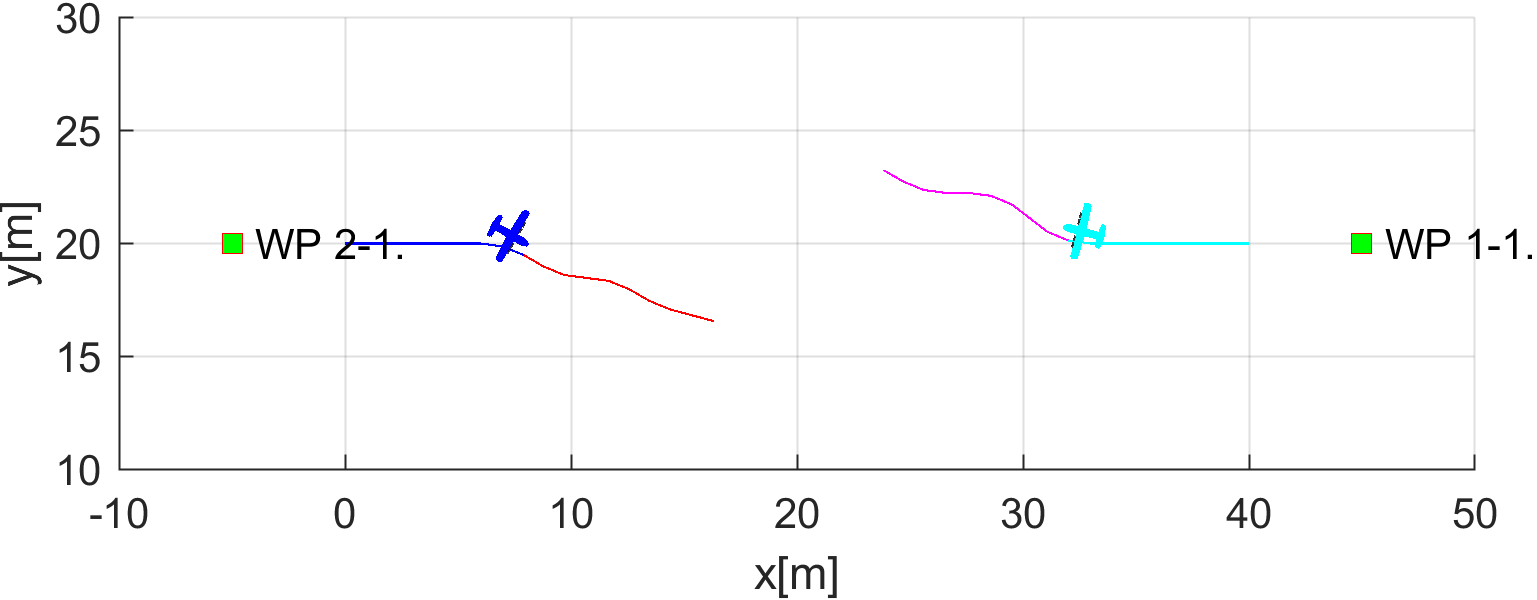
\includegraphics[width=0.9\linewidth]{\FIGDIR/NS055UtmCooperativeHeadOn00008}
        \caption{Collision case creation.}
        \label{fig:ruleBasedHeadOnSituationCollisionCaseCreation}
    \end{subfigure}
    \\
    \begin{subfigure}{0.75\textwidth}
        \centering
        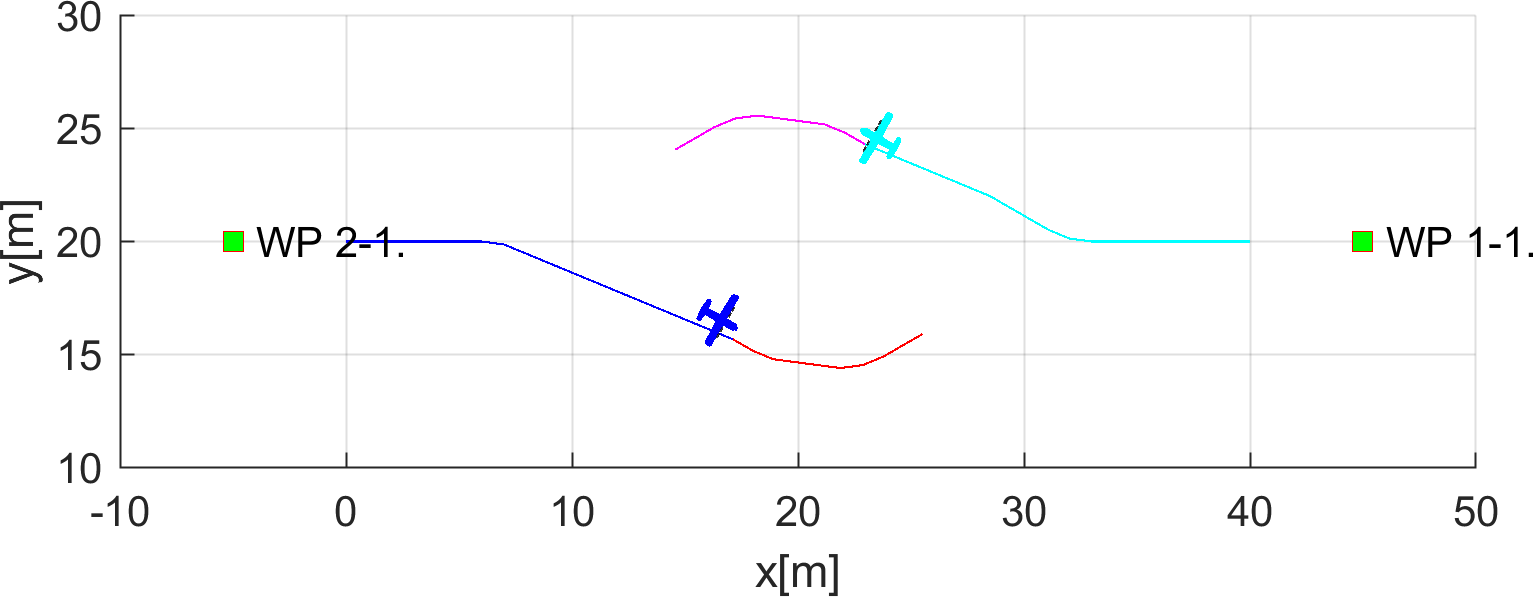
\includegraphics[width=0.9\linewidth]{\FIGDIR/NS056UtmCooperativeHeadOn00018} 
        \caption{Well clear before.}
        \label{fig:ruleBasedHeadOnWellClearBefore}
    \end{subfigure}
    \\
    \begin{subfigure}{0.75\textwidth}
        \centering
        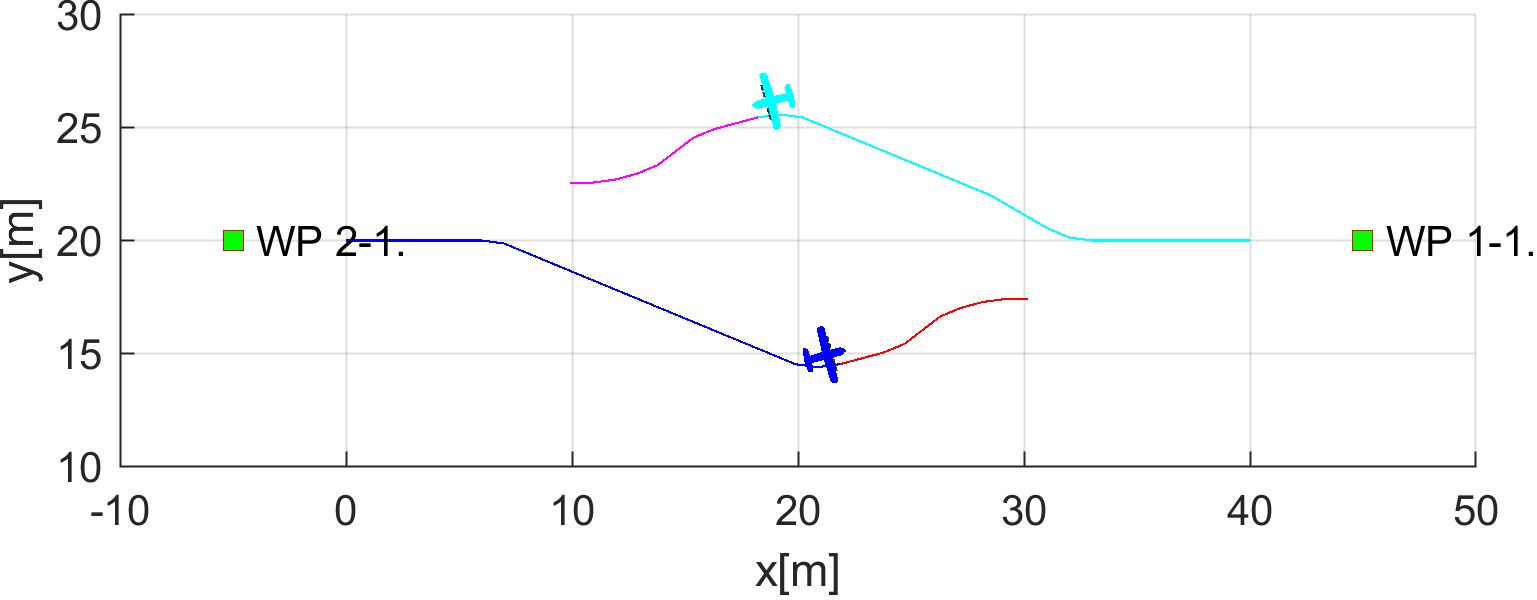
\includegraphics[width=0.9\linewidth]{\FIGDIR/NS057UtmCooperativeHeadOn00023} 
        \caption{Well clear after.}
        \label{fig:ruleBasedHeadOnWellClearAfter}
    \end{subfigure}
    \\
    \begin{subfigure}{0.75\textwidth}
        \centering
        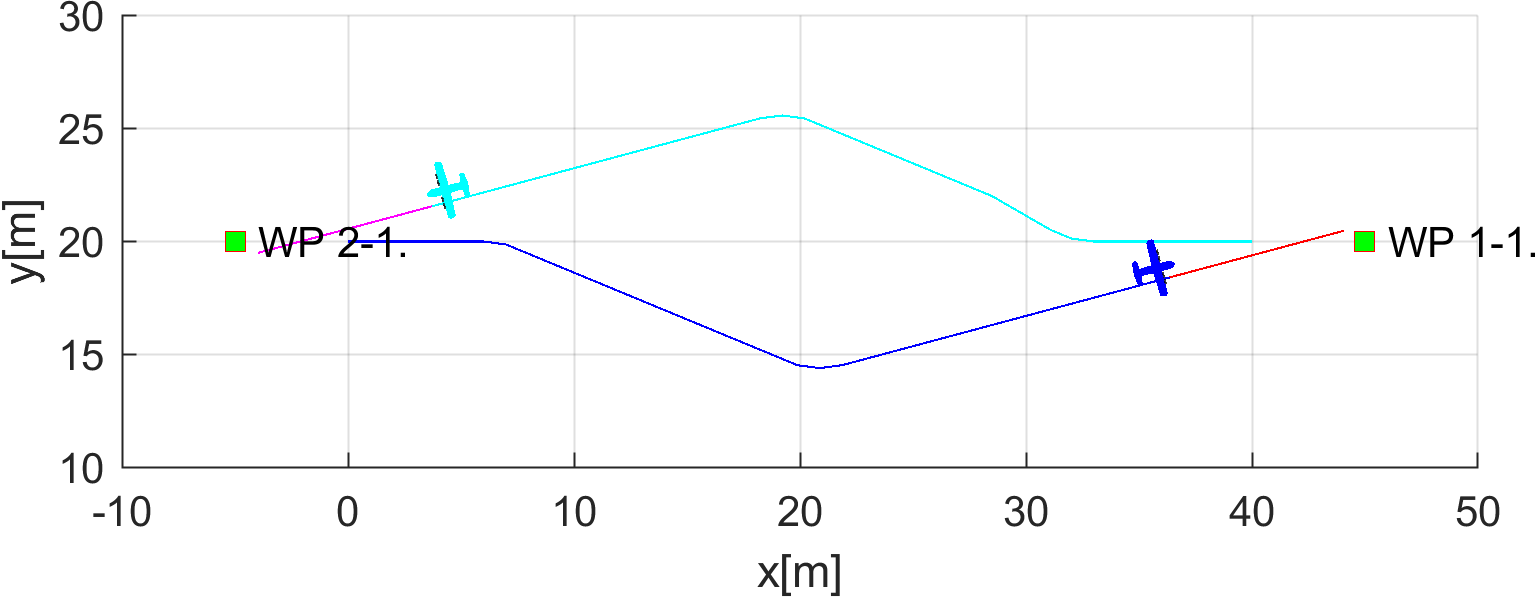
\includegraphics[width=0.9\linewidth]{\FIGDIR/NS058UtmCooperativeHeadOn00038} 
        \caption{Waypoints reach.}
        \label{fig:ruleBasedHeadOnWaypointsReach}
    \end{subfigure}
    \caption{Test scenario for \emph{Rule based head on approach} (virtual roundabout). }
    \label{fig:testCaseRuleBasedHeadOnApproach}
\end{figure}

\paragraph{Collision Case Calculation: } For test scenario in (fig. \ref{fig:testCaseRuleBasedHeadOnApproach}) where UAS 1 (blue) have head on collision with UAS 2 (cyan), \emph{Collision Case} have been calculated (tab. \ref{tab:collisionCasesRuleBasedHeadon}).

The \emph{Collision point} is at $[20,20,0]^T$ in Flight Level $FL450$ coordinate frame.

The \emph{angle of approach} was evaluated as $180^{\circ}$ which indicates \emph{Head on Approach} due the $130^\circ \le angle of Approach \le 180^\circ$ condition.

The \emph{mutual position} of UAS 1 (blue) and UAS 2 (cyan) is giving the roles of \emph{Roundabout} to \emph{both} UAS.

The \emph{safety margin} for \emph{Well Clear} was determined as $5m$ for UAS 1 and UAS 2. The combined \emph{Case Margin} is 10 m, which is sum of both. The \emph{mutual distance} can not go below this threshold.


\begin{table}[H]
    \centering
    \begin{tabular}{c|c|c|c|c|c||c|c}
        \multicolumn{6}{c||}{Collision Case}& \multicolumn{2}{c}{Margins} \\ \hline
        id  & UAS & role & \begin{tabular}[c]{@{}c@{}}collision\\ point\end{tabular} & \begin{tabular}[c]{@{}c@{}}angle of\\ approach\end{tabular} & type&  safety  & case  \\ \hline\hline
        % Case 1-2
        \multirow{2}{*}{1-2} & 1   & Roundabout & \multirow{2}{*}{$[20,20,0]^T$} & \multirow{2}{*}{$180^\circ$} & \multirow{2}{*}{Head on} & 5 & \multirow{2}{*}{10} \\ \cline{2-3} \cline{7-7} & 2   & Roundabout & & & & 5 & 
    \end{tabular}
    \caption{Collision case for \emph{Rule-based head on} scenario.}
    \label{tab:collisionCasesRuleBasedHeadon}
\end{table}

\paragraph{Distance to Safety Margin Evolution:} The safety margin values (well clear) (fig. \ref{fig:testCaseRuleBasedHeadOnAvoidancePerformance}) in controlled airspace are much larger than in non-controlled airspace (near miss) (fig. \ref{fig:testCaseHeadOnAvoidancePerformance}).

The enforced rule was (rule \ref{tab:ruleHeadonApproach}) with parameters: Collision Point $[20,20,0]^T$ and \emph{Safety Margin} $10$ $m$ as given by Collision Case (tab. \ref{tab:collisionCasesRuleBasedHeadon}).

The mutual \emph{UAS distance} (blue line) does not go over \emph{Safety Margin} (red line) which means  both UAS well clear margins are not broken by any means (fig. \ref{fig:testCaseRuleBasedHeadOnApproach}).


\begin{figure}[H]
    \centering
    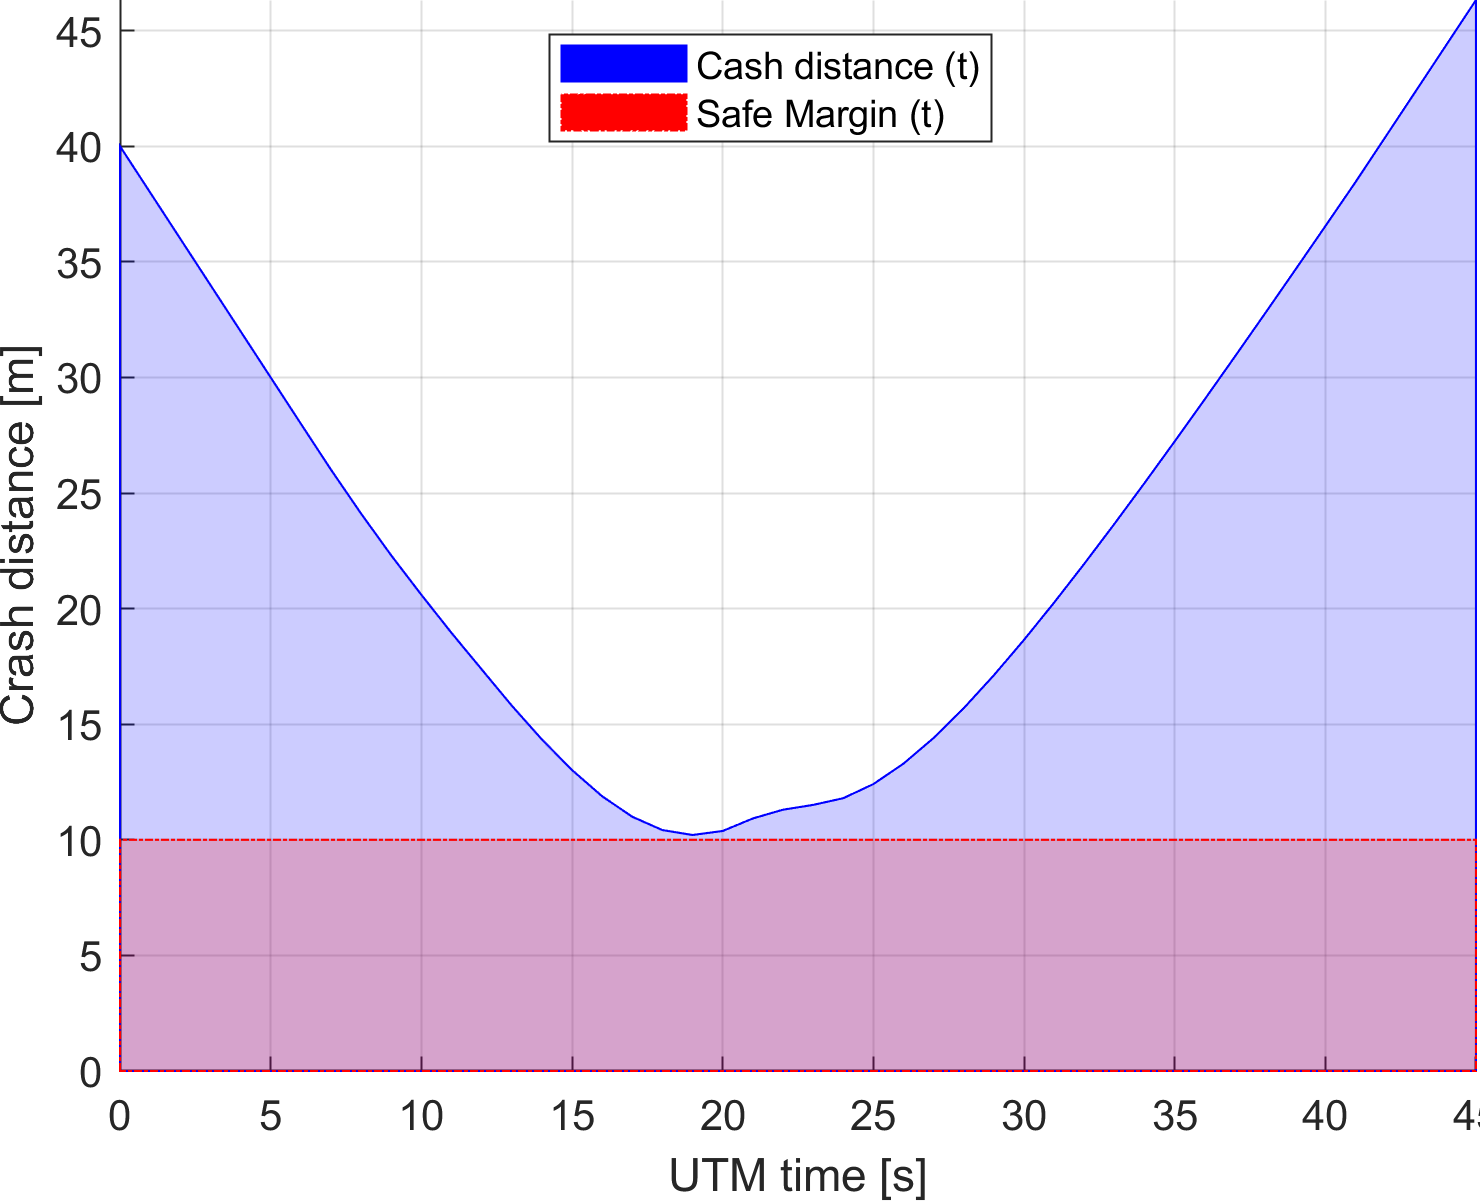
\includegraphics[width=0.55\linewidth]{\FIGDIR/NS059UtmCooperativeHeadOnPerformance} 
    \caption{Distance to safety margin evolution for \emph{rule based head on scenario}.}
    \label{fig:testCaseRuleBasedHeadOnAvoidancePerformance}
\end{figure}


\paragraph{Distance to Safety Margin Peaks:} Given by (tab. \ref{tab:testCaseRuleBasedHeadOnSafetyMarginDistances}) represents the proximity on UAS mutual distance to \emph{well clear condition} breach. The breach of \emph{well clear condition} was not achieved. The \emph{minimal distance to safety margin} was $0.2084$ $m$. The \emph{maximal distance to safety margin} was $36.3253 m$ which represents distance at \emph{Collision Case} closing. 

\begin{table}[H]
    \centering
    \begin{tabular}{c||c|c|c}
        \multirow{2}{*}{UAS:} & \multicolumn{3}{c}{Distance to Safety Margin} \\ \cline{2-4} 
                  & min          & max         & breach         \\ \hline\hline
            1-2   & 0.2084       & 36.3253     & false          \\ 
    \end{tabular}
    \caption{\emph{Rule based head on} safety margin distances.}
    \label{tab:testCaseRuleBasedHeadOnSafetyMarginDistances}
\end{table}

\paragraph{Path Tracking Performance:} \emph{Path tracking} is displayed in (fig. \ref{fig:ruleBasedHeadOnTrajectoryTrackingPerformance}). The \emph{UAS} trajectory is divined into \emph{X, Y, Z axis tracking over UTM Time}. The \emph{Reference Trajectory} (green dashed line) interconnect starting position of UAS (green square marked S) an goal waypoint (green square marked 1). The \emph{Executed Trajectory} (blue solid line) reflects real UAS trajectory. 

\begin{enumerate}
    \item UAS 1. (fig, \ref{fig:ruleBasedHeadOnUAS1PathTracking}) do steady right side \emph{roundabout maneuver} (y-axis).
    
    \item UAS 2. (fig. \ref{fig:ruleBasedHeadOnUAS2PathTracking}) do steady right side \emph{roundabout maneuver} (y-axis).
\end{enumerate}

\begin{figure}[H]
	\centering
    \begin{subfigure}{0.48\textwidth}
    	\centering
        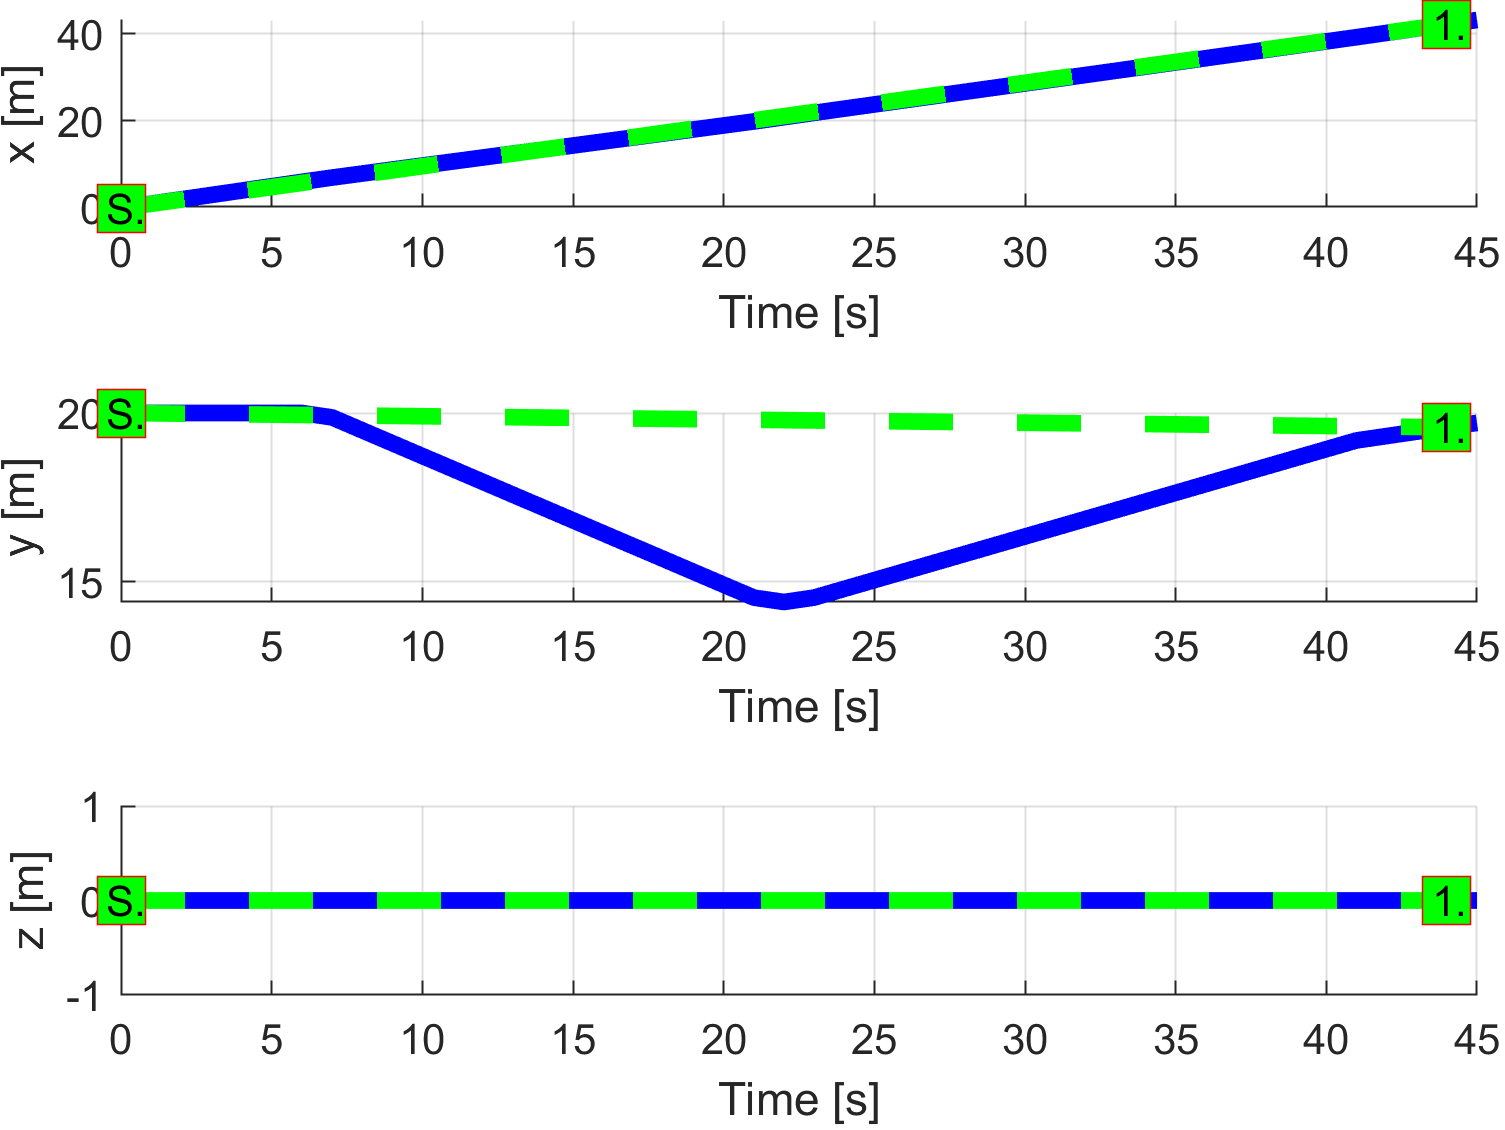
\includegraphics[width=0.9\linewidth]{\FIGDIR/NS060UtmCooperativeHeadOnUAV1PathFollowing}
        \caption{UAS 1.}
        \label{fig:ruleBasedHeadOnUAS1PathTracking}
    \end{subfigure}
    \begin{subfigure}{0.48\textwidth}
    	\centering
        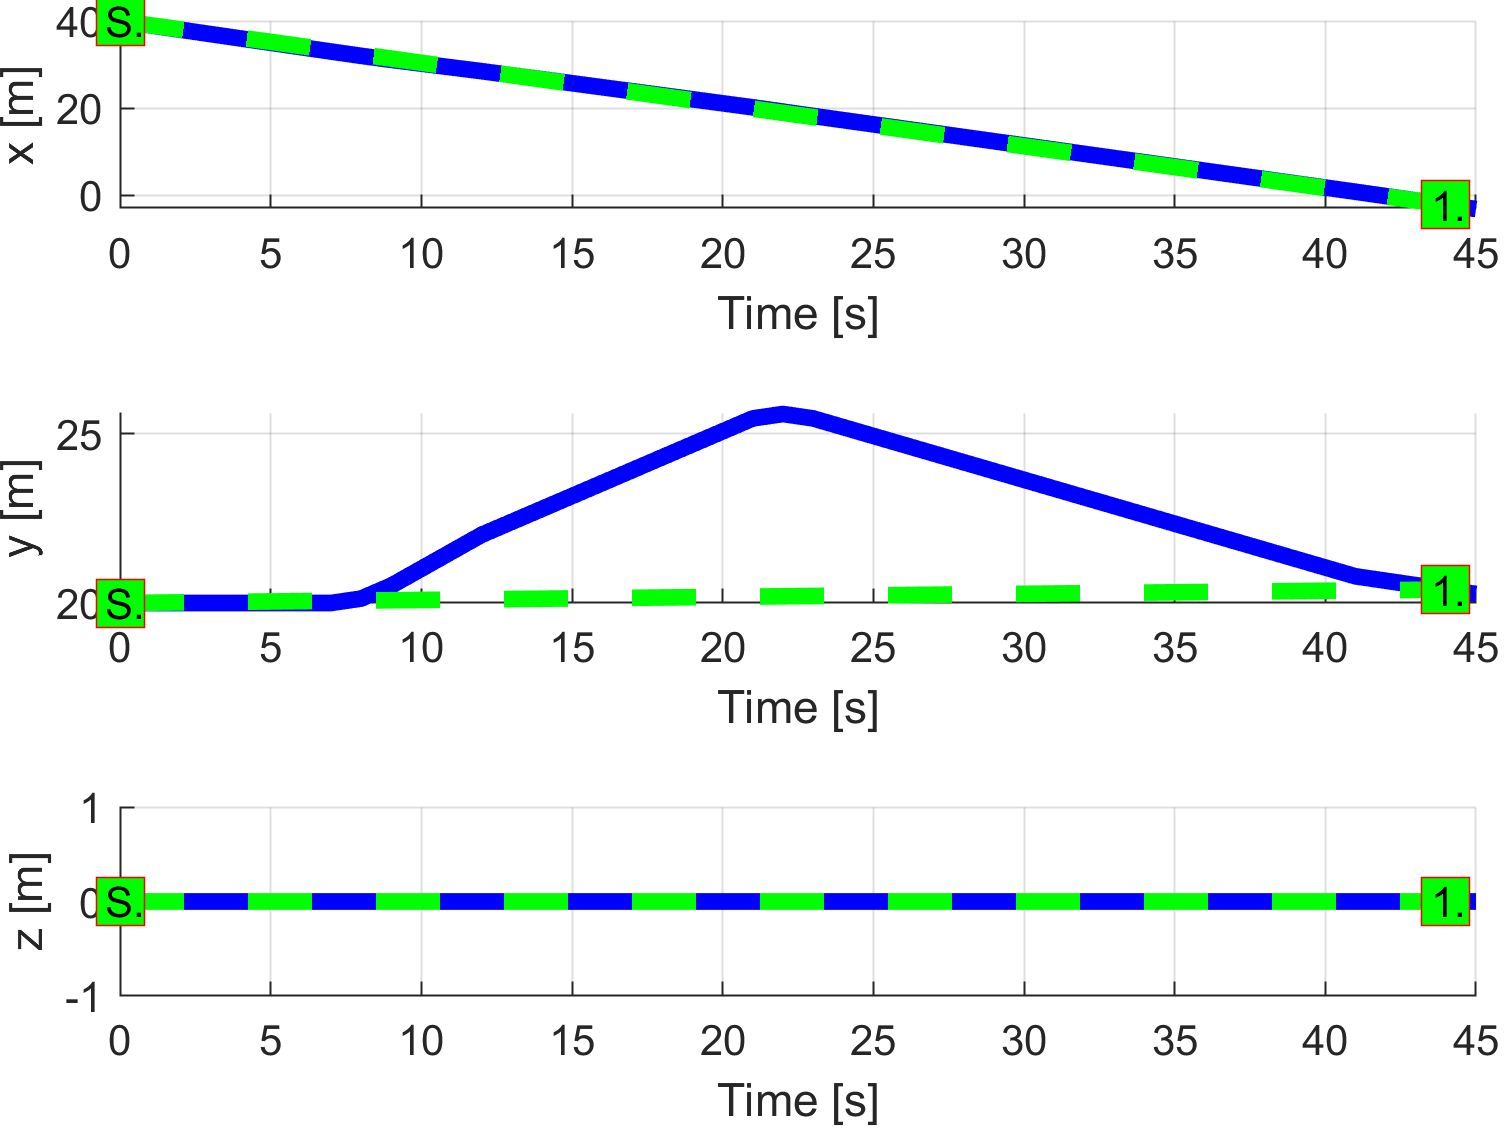
\includegraphics[width=0.9\linewidth]{\FIGDIR/NS061UtmCooperativeHeadOnUAV2PathFollowing} 
        \caption{UAS 2.}
        \label{fig:ruleBasedHeadOnUAS2PathTracking}
    \end{subfigure}
    \caption{\emph{Trajectory tracking} for \emph{Rule based head on} test case. }
    \label{fig:ruleBasedHeadOnTrajectoryTrackingPerformance}
\end{figure}

\paragraph{Path Tracking Deviations:} Deviations (tab. \ref{tab:pathTrackingParametersForRuleBasedHeadOn}) are in \emph{expected ranges}, considering the \emph{mission plans} (tab. \ref{tab:missionSetupRuleBasedHeadOnScenario}) and \emph{Collision Case} safety margin of $10 m$.

\begin{table}[H]
    \centering
    \begin{tabular}{c||c|c}
        \multirow{2}{*}{Param.} & UAS 1     & UAS 2              \\\cline{2-3}
                        & $\mathscr{WP}_1$  & $\mathscr{WP}_1$   \\\hline\hline
          $\max |x|$    & 0                 & 0                  \\\hline
          $\max |y|$    & 5.40              & 5.40              \\\hline
          $\max |z|$    & 0                 & 0                  \\\hline
          $\max dist.$  & 5.40              & 5.40              \\
    \end{tabular}
    \caption{Path tracking properties for \emph{Rule based head on} scenario.}
    \label{tab:pathTrackingParametersForRuleBasedHeadOn}
\end{table}

% 09 Rule Based Head On
\paragraph{Computation Load:} The \emph{computation load} for \emph{scenario} (fig.\ref{fig:ruleBasedHeadOnComputationTime}) shows used time (y-axis) over decision frame (x-axis).

\begin{figure}[H]
    \centering
    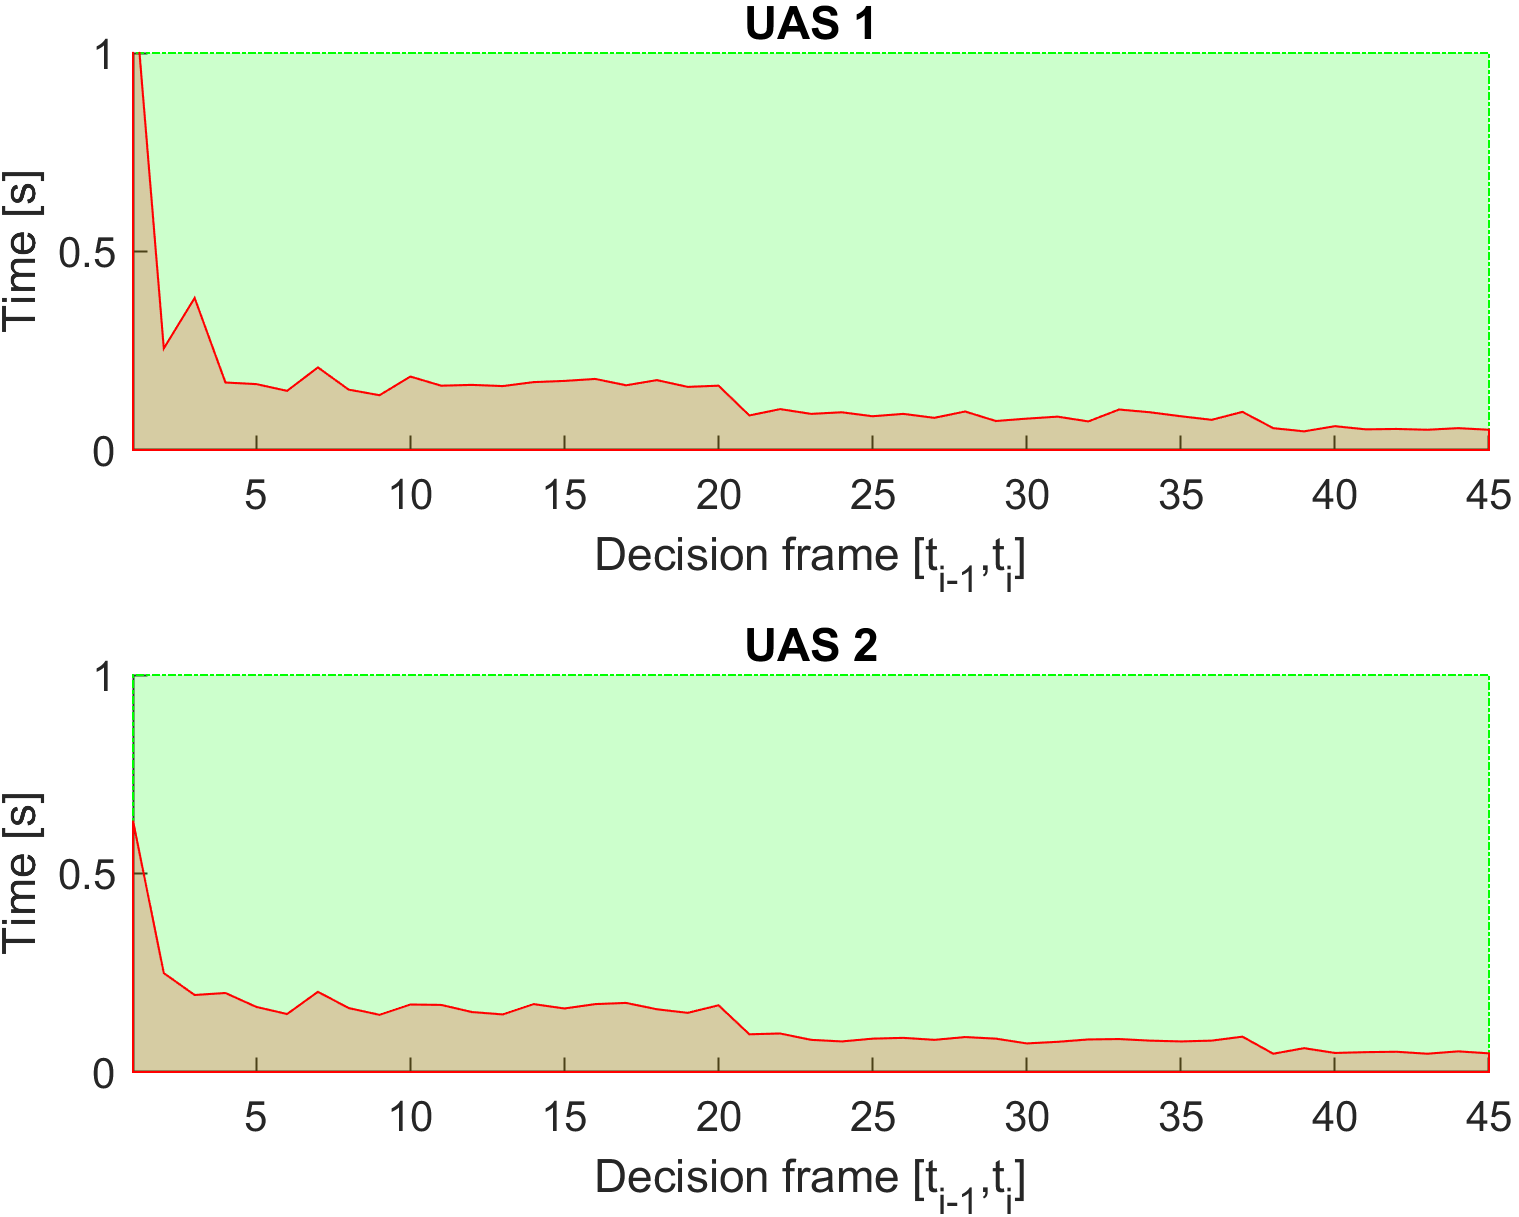
\includegraphics[width=0.65\linewidth]{\FIGDIR/NS100RuleBasedHeadOnComputationTime} 
    \caption{Computation time for \emph{Rule-based head on} scenario.}
    \label{fig:ruleBasedHeadOnComputationTime}
\end{figure}
    	\subsection{Rule-Based Mixed Head-On with Converging}\label{s:testRuleMixed}

\paragraph{Scenario:} Four \emph{UAS} are approaching an airway \emph{intersection} at the \emph{same time} from \emph{opposite direction} in \emph{controlled airspace} (over 500 feet Above Ground Level). Each \emph{UAS} have following \emph{Collision Hazards}:
\begin{enumerate}
	\item \emph{Head on Collision Hazard} - An UAS is approaching from opposite direction which invokes need to avoid \emph{Collision Point} actively

	\item \emph{Active Converging Collision Hazard} -  An UAS is approaching from the \emph{right side}, which gives him \emph{Right of the Way} and invokes the need to avoid \emph{Intruder} actively.

	\item \emph{Passive Converging Collision Hazard} - An UAS is approaching from the \emph{left side}, which gave us \emph{Right of the Way} and imposes an obligation of \emph{active avoidance} on other \emph{UAS}.
\end{enumerate}

\begin{note}
	Presented scenario is \emph{the worst possible situation} in current \emph{manned aviation ATM}. 
\end{note}

\noindent\emph{Mentioned Collision Hazards} must be addressed by \emph{UTM} service in the following manner:

\begin{enumerate}
	\item \emph{Each UAS} in particular \emph{Controlled Space} periodically sends synchronized \emph{Position Notification} messages (tab. \ref{tab:positionNotification}). 
	
	\item \emph{UTM} service receives \emph{Position Notifications} and manages \emph{Collision Cases} (tab. \ref{tab:collisionCase}) in \emph{Controlled Space}. 
	
	\item \emph{UTM} detects multiple \emph{Collision Cases} with \emph{Collision Points} in  the vicinity.
	
	\item \emph{UTM} service creates \emph{Virtual Roundabout} and implements \emph{Normative Directive} on all \emph{UAS} in the area.
\end{enumerate}

\noindent\emph{Mission parameters} for four UAS systems are defined in (tab. \ref{tab:missionSetupRuleBasedMixedScenario}).

\begin{table}[H]
	\centering
	\begin{tabular}{c||c|c||c}
		\multirow{2}{*}{UAS} &\multicolumn{2}{c||}{Position} & \multirow{2}{*}{$\mathscr{WP}_1$} \\\cline{2-3}
		  & $[x,y,z]$           & $[\theta,\varpi,\psi]$           & \\\hline\hline
		1 & $[0,20,0]^T $       & $[0^\circ,0^\circ,0^\circ]^T$    & $[45,20,0]^T$\\\hline 
		2 & $[40,20,0]^T $       & $[0^\circ,0^\circ,180^\circ]^T$    & $[-5,20,0]^T$\\\hline 
		3 & $[20,0,0]^T $       & $[0^\circ,0^\circ,90^\circ]^T$    & $[20,45,0]^T$\\\hline 
		4 & $[20,40,0]^T $       & $[0^\circ,0^\circ,-90^\circ]^T$  & $[45,20,0]^T$\\ 
	\end{tabular}
	\caption{Mission setup for \emph{rule-based mixed} scenario.}
	\label{tab:missionSetupRuleBasedMixedScenario}
\end{table}

\paragraph{Assumptions:} Following assumptions are valid for this test:

\begin{enumerate}
	\item \emph{Controlled Airspace Airworthiness} - UAS system is equipped with necessary controlled airspace equipment like ADS-B In/Out, Radar, Transponder, etc. Moreover, airworthy \emph{UAS} has capability to precisely follow \emph{UTM directives} (max. 5 $\%$ deviation).
	
	\item \emph{C2 (Command \& control) Link Established} - necessary for (UAS $\leftrightarrow$ UAS) and (UAS $\leftrightarrow$ UTM) communication. If \emph{C2} link is lost the \emph{UAS} will enter into \emph{Emergency avoidance mode}.
	
	\item \emph{Decision frame synchronization with UTM} - necessary in discrete C2 environment otherwise \emph{safety margins} needs to be \emph{bloated}.
	
	\item \emph{Every UAS have identical cruising speed} - simplification impacting \emph{UTM} service implementation. \emph{Obstacle Avoidance Framework} can comprehend various intruders speed, with proper \emph{UAS} directives.
\end{enumerate}

\paragraph{Main Goal:} Show possibility of \emph{Virtual Roundabout} invoked by \emph{UTM} directives where \emph{Obstacle Avoidance Framework based on Reach Sets} is used as a \emph{Navigation Module}.

\paragraph{Acceptance  Criteria:} Following criteria must be met:

\begin{enumerate}
	\item \emph{Well Clear Condition valid for every UAS} - Each \emph{UAS} must have \emph{minimal required distance} from \emph{other UAS} for all \emph{Virtual Roundabout} enforcement time.
	
	\item \emph{Fulfillment of UTM Directives} - Each UAS must stay in a \emph{Navigation mode} for all \emph{Virtual Roundabout} enforcement time. Each \emph{UAS} must stay on \emph{Virtual Roundabout} for the necessary time, before leaving for \emph{Original Navigation waypoint $\mathscr{WP}_1$}.
\end{enumerate}

\paragraph{Testing Setup:} The \emph{standard test setup} for each UAS defined in (tab. \ref{tab:testMovementOrientations}, \ref{tab:testUASBasicParameters}, \ref{tab:testNavigationGridBasic}, \ref{tab:testAvoidanceGridBasic}, \ref{tab:testUASColoring}) is used with following parameter override:
\begin{enumerate}
	\item \emph{Navigation grid - type} - \emph{ACAS-like} with \emph{horizontal enabled maneuvers}
\end{enumerate}

This \emph{configuration} is based on the assumption that every UAS is in \emph{controlled airspace} in \emph{FL450} (flight level 45000 feet Above Sea Level), without permission for a \emph{climb or descent maneuver}. The \emph{rule engine} is initialized in standard \emph{Rules of the air} configuration (fig. \ref{fig:RuleEngineInstanceLevels}).

There is \emph{UTM} service for given \emph{airspace cluster} calculating \emph{collision cases} (tab. \ref{tab:collisionCase}) based on incoming \emph{UAS position notifications} (tab. \ref{tab:positionNotification}).

\paragraph{Simulation Run:} Notable moments from the \emph{simulation run} (fig. \ref{fig:testCaseRuleBasedMixed}) are the following:

\begin{enumerate}
	\item \emph{Collision cases created} (fig. \ref{fig:ruleMultipleCollisionCasesCreated}) following events happen in this step:
	\begin{enumerate}[a.]
		\item Four \emph{UAS} are approaching airways intersection: \emph{UAS 1} (blue) from left, \emph{UAS 2} (cyan) from right, \emph{UAS 3} (green) from the bottom, \emph{UAS 4} (black) from the top.
		
		\item They are going to collide at point $[20,20,0]^T$ of \emph{Flight level} (elevation is 45, 000 feet Above Mean Sea Level).
		
		\item \emph{UTM service} notices future \emph{Collision Situations} and creates \emph{Collision Cases}.
		
		\item There are many \emph{Collision Cases} in the near vicinity. The \emph{Virtual Roundabout} is created with \emph{Safety margin} $15$ $m$.
		
		\item The \emph{UTM} service then sends a new \emph{Roundabout Directives} to involved \emph{UAS} systems.
		
		\item Each \emph{UAS} starts \emph{Roundabout Entry Maneuver} by correcting own  \emph{Heading} and \emph{Speed} (if its necessary).
	\end{enumerate}   
	
	\item \emph{Roundabout entry} (fig. \ref{fig:ruleMultipleRoundabountEntry}) - Each \emph{UAS} enters into \emph{Virtual Roundabout} while sending \emph{Roundabout Entrance Notification} to \emph{UTM service}.
	
	\item \emph{Roundabout leave} (fig. \ref{fig:ruleMultipleRoundaboutLeave})  following events happens in this step:
	\begin{enumerate}[a.]
		\item Each \emph{UAS} when is going to approach the level of \emph{Original Goal Waypoint} sends \emph{Roundabout Leave Request}.
		
		\item UTM system will check if there is \emph{Sufficient Free Space} to leave \emph{Virtual Roundabout}.
		
		\item The \emph{UTM Service then issues} \emph{Virtual Roundabout Leave Approval}.
		
		\item Each \emph{UAS} will correct own heading and speed in the range of received permit.
	\end{enumerate}   
	
	\item \emph{Situation resolution} (fig. \ref{fig:ruleMultipleSituationResolution}) - Each \emph{UAS} is heading away from \emph{Roundabout Center}, there is no active user of \emph{Virtual Roundabout}. \emph{UTM} will remove \emph{Virtual Roundabout}  and closes underlying \emph{Collision Cases}. Each \emph{UAS} will reach respective \emph{Original Goal Waypoint}.
\end{enumerate}


\begin{figure}[H]
	\centering
	\begin{subfigure}{0.48\textwidth}
		\centering
		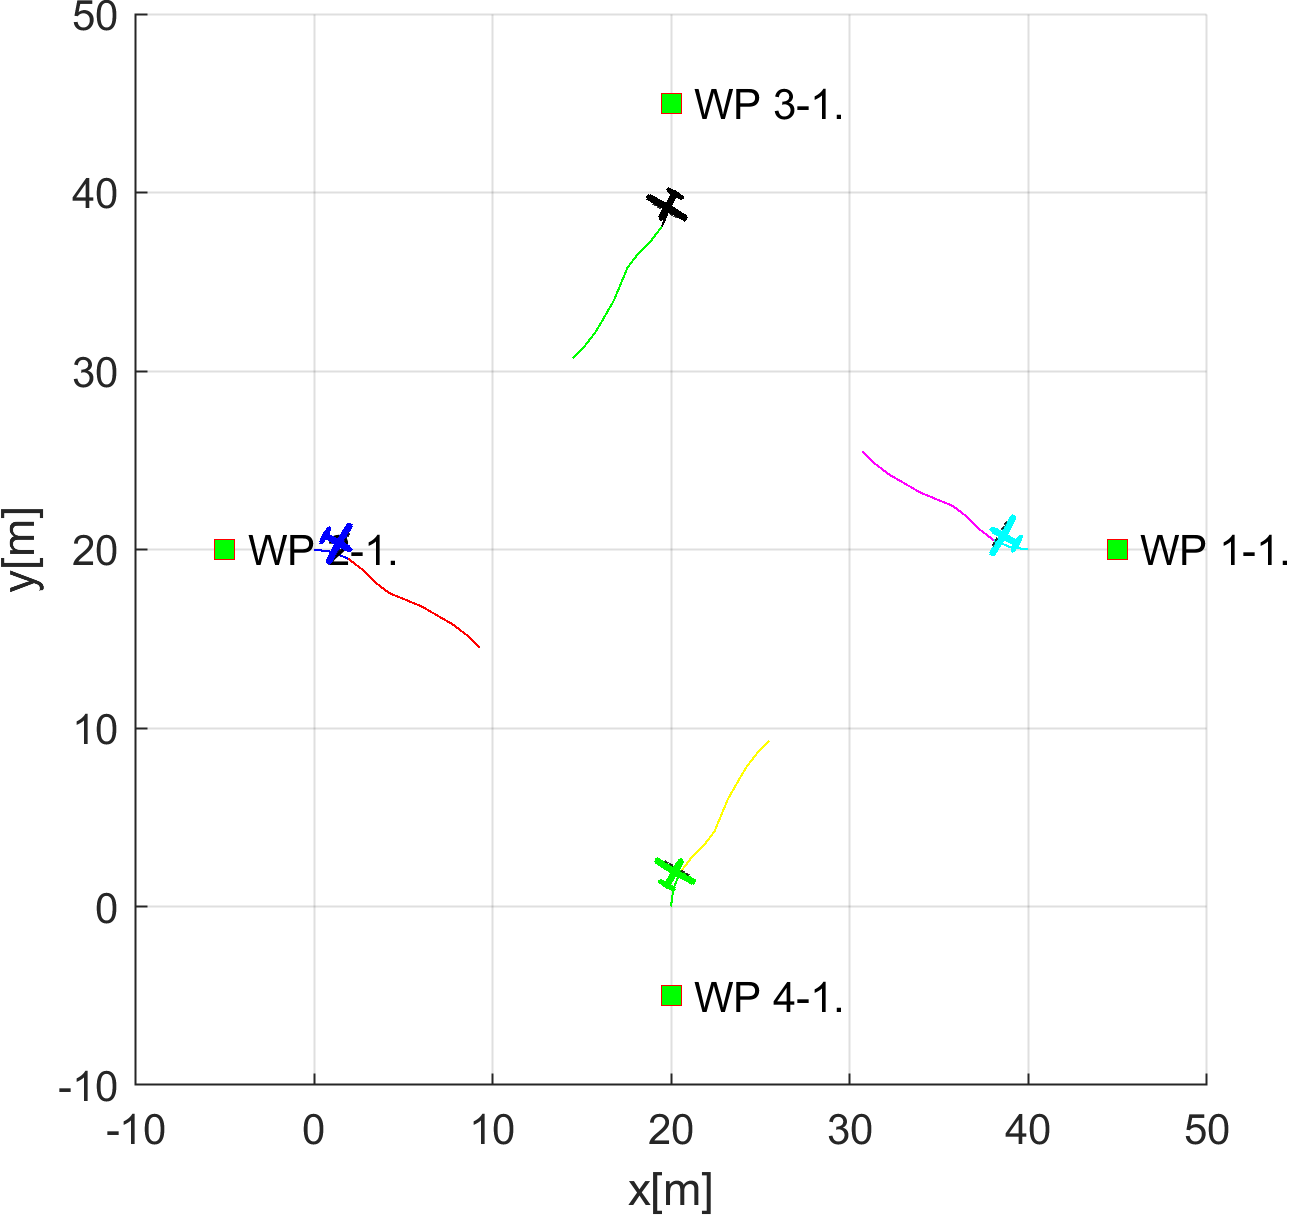
\includegraphics[width=0.9\linewidth]{\FIGDIR/NS062UtmCooperativeHeadOnMultiple00002}
		\caption{Collision cases created.}
		\label{fig:ruleMultipleCollisionCasesCreated}
	\end{subfigure}
	\begin{subfigure}{0.48\textwidth}
		\centering
		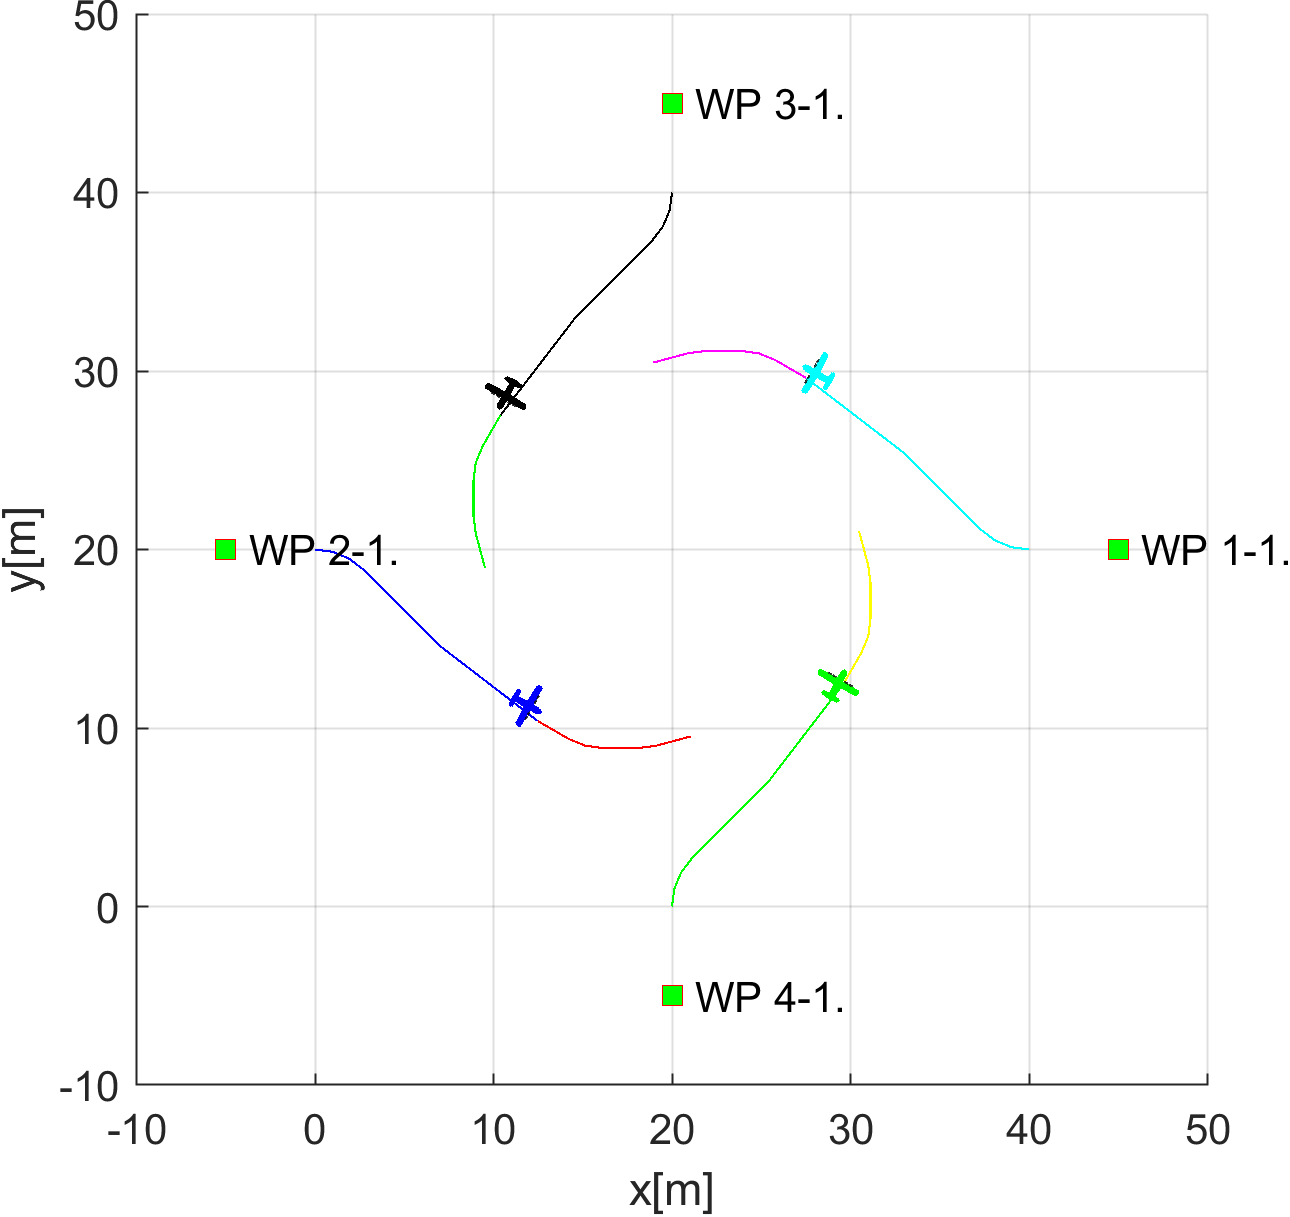
\includegraphics[width=0.9\linewidth]{\FIGDIR/NS063UtmCooperativeHeadOnMultiple00016} 
		\caption{Roundabout entry.}
		\label{fig:ruleMultipleRoundabountEntry}
	\end{subfigure}
	\\
	\begin{subfigure}{0.48\textwidth}
		\centering
		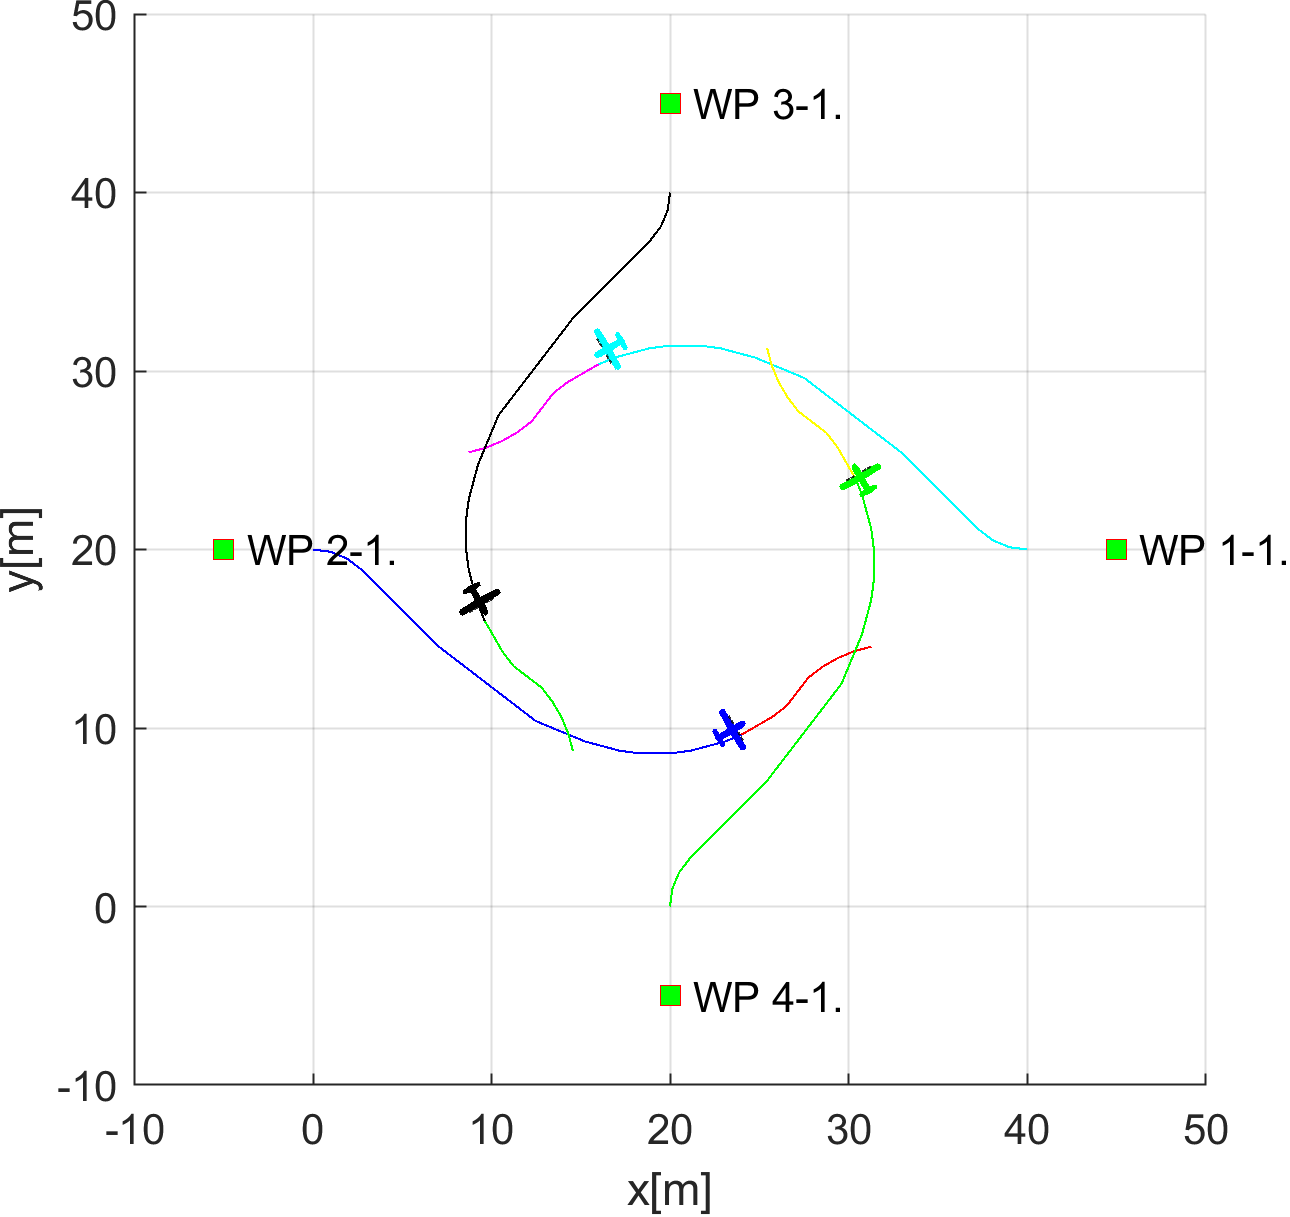
\includegraphics[width=0.9\linewidth]{\FIGDIR/NS064UtmCooperativeHeadOnMultiple00028} 
		\caption{Roundabout leave.}
		\label{fig:ruleMultipleRoundaboutLeave}
	\end{subfigure}
	\begin{subfigure}{0.48\textwidth}
		\centering
		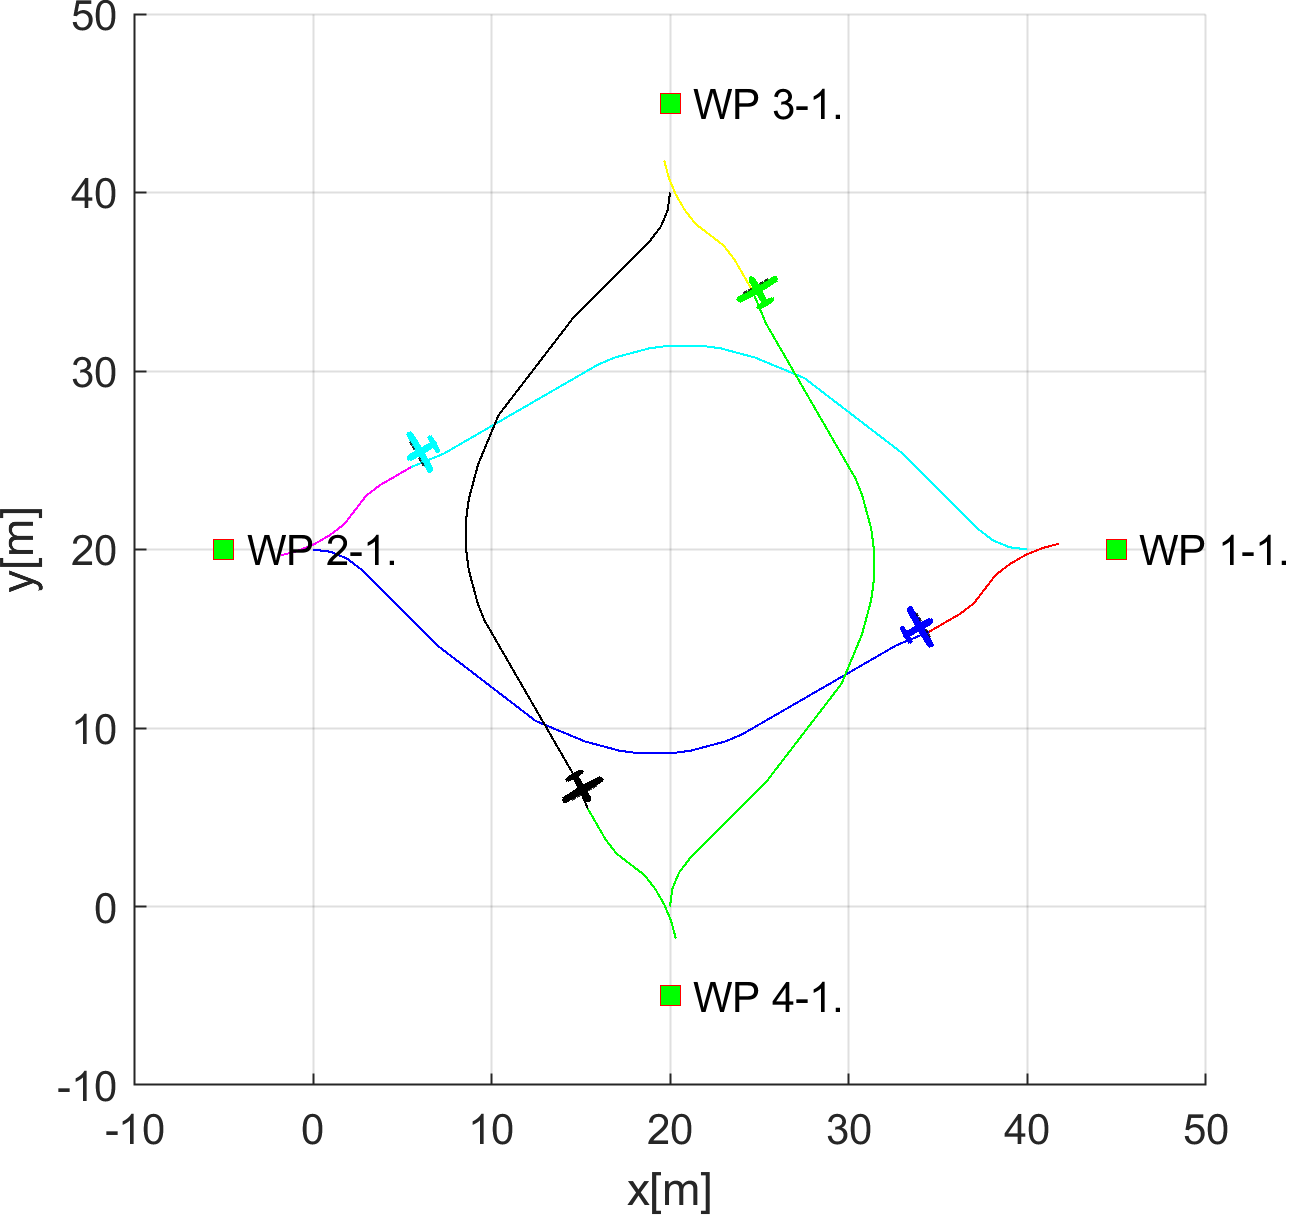
\includegraphics[width=0.9\linewidth]{\FIGDIR/NS065UtmCooperativeHeadOnMultiple00040} 
		\caption{Situation resolution.}
		\label{fig:ruleMultipleSituationResolution}
	\end{subfigure}
	\caption{Test scenario for \emph{rule-based mixed} situation with the \emph{self-separation mode}.}
	\label{fig:testCaseRuleBasedMixed}
\end{figure}

\paragraph{Collision Cases Calculation:} The set of original \emph{Collision cases} is given in (tab. \ref{tab:collisionCasesRuleBasedMixed}). 

Each \emph{UAS} has one \emph{Head on}, \emph{Converging passive}, \emph{Converging active} collision hazard. For example \emph{UAS 1} have a \emph{head-on} with  \emph{UAS 2}, \emph{converging passive} with \emph{UAS 4}, \emph{converging active} with \emph{UAS 3}. For \emph{UAS 2-4} check \emph{role} in respective \emph{Collision Cases}.

\begin{note} \emph{Collision cases} calculated by \emph{UTM} are symmetric, which means that collision case for \emph{UAS X, UAS Y} is identical to collision case calculated for \emph{UAS Y, UAS X}, $X \neq Y$.
\end{note}

\emph{Safety margin} representing \emph{Well Clear Margin} for single \emph{UAS} in \emph{Collision Case} ranges $5-8$ $m$. \emph{Case margin} representing the minimal mutual distance between two \emph{UAS systems} to remain well clear ranges $12-15$ $m$.

\emph{Merged Collision Case} is oversimplified for demonstration purposes. \emph{Merge Case Procedure} is out of the scope of this work due to its extent. Every \emph{Collision Case} shares same \emph{Collision Point} $[20,20,0]^T$ in flight level coordinate frame. \emph{Merged Collision Case} type was set as \emph{Roundabout}, due the number of collision case \emph{attendants} is greater than 2. Each \emph{UAS role} has been set as \emph{Roundabout}. The enforced \emph{safety margin} is equal to $15$ $m$, which is the maximum of all \emph{single collision case combined margins}.

\begin{table}[H]
	\centering
	\begin{tabular}{c|c|c|c|c|c||c|c}
		\multicolumn{6}{c||}{Collision Case}& \multicolumn{2}{c}{Margins} \\ \hline
		id  & UAS & role & \begin{tabular}[c]{@{}c@{}}collision\\ point\end{tabular} & \begin{tabular}[c]{@{}c@{}}angle of\\ approach\end{tabular} & type&  safety  & case  \\ \hline\hline
		% Case 1-2
		\multirow{2}{*}{1-2} & 1   & Roundabout & \multirow{2}{*}{$[20,20,0]^T$} & \multirow{2}{*}{$180^\circ$} & \multirow{2}{*}{Head on} & 8 & \multirow{2}{*}{15} \\ \cline{2-3} \cline{7-7} & 2   & Roundabout & & & & 7& \\ \hline
		% Case 1-3
		\multirow{2}{*}{1-3} & 1   & Converging & \multirow{2}{*}{$[20,20,0]^T$} & \multirow{2}{*}{$90^\circ$} & \multirow{2}{*}{Converging} & 8 & \multirow{2}{*}{15} \\ \cline{2-3} \cline{7-7} & 3   & Right o.W. & & & & 5& \\ \hline
		% Case 1-4
		\multirow{2}{*}{1-4} & 1   & Right o.W. & \multirow{2}{*}{$[20,20,0]^T$} & \multirow{2}{*}{$90^\circ$} & \multirow{2}{*}{Converging} & 8 & \multirow{2}{*}{15} \\ \cline{2-3} \cline{7-7} & 4   & Converging & & & & 5& \\ \hline
		% Case 2-3
		\multirow{2}{*}{2-3} & 2   & Right o.W. & \multirow{2}{*}{$[20,20,0]^T$} & \multirow{2}{*}{$90^\circ$} & \multirow{2}{*}{Converging} & 7 & \multirow{2}{*}{12} \\ \cline{2-3} \cline{7-7} & 3   & Converging & & & & 5& \\ \hline
		% Case 2-4
		\multirow{2}{*}{2-4} & 2   & Converging & \multirow{2}{*}{$[20,20,0]^T$} & \multirow{2}{*}{$90^\circ$} & \multirow{2}{*}{Converging} & 7 & \multirow{2}{*}{12} \\ \cline{2-3} \cline{7-7} & 4   & Right o.W. & & & & 5& \\ \hline
		% Case 3-4
		\multirow{2}{*}{3-4} & 3   & Roundabout & \multirow{2}{*}{$[20,20,0]^T$} & \multirow{2}{*}{$180^\circ$} & \multirow{2}{*}{Head on} & 7 & \multirow{2}{*}{14} \\ \cline{2-3} \cline{7-7} & 4   & Roundabout & & & & 7& \\\hline\hline
		% Merged case - header 
		\multicolumn{6}{c||}{Merged cases} & \multicolumn{2}{c}{\multirow{2}{*}{\begin{tabular}[c]{@{}c@{}}  Safety \\ Margin\end{tabular}}} \\ \cline{1-6} 
		id & UAS & role & \multicolumn{2}{c|}{collision point} & type& \multicolumn{2}{c}{} \\ \hline\hline
		% line 1
		\multirow{4}{*}{\begin{tabular}[c]{@{}c@{}}1-2-\\ -3-4\end{tabular}} & 1   & Roundabout & \multicolumn{2}{c|}{\multirow{4}{*}{$[20,20,0]^T$}} & \multirow{4}{*}{Roundabout} & \multicolumn{2}{c}{\multirow{4}{*}{15}} \\ \cline{2-3}
		% line 2
		& 2   & Roundabout & \multicolumn{2}{c|}{} & & \multicolumn{2}{c}{}\\ \cline{2-3}
		% line 3
		& 3   & Roundabout & \multicolumn{2}{c|}{} & & \multicolumn{2}{c}{}\\ \cline{2-3}
		% line 4
		& 4   & Roundabout & \multicolumn{2}{c|}{} & & \multicolumn{2}{c}{}\\ 
	\end{tabular}
	\caption{Collision cases for \emph{rule-based mixed} scenario.}
	\label{tab:collisionCasesRuleBasedMixed}
\end{table}

\newpage
\paragraph{Distance to Safety Margin Evolution:} \emph{Merged Collision Case Safety Margin} is $15$ $m$, and it is valid for all \emph{UAS mutual distances}. The simple condition for \emph{Remain Well Clear} is:

\begin{equation*}
	crashDistance(UAS_X,UAS_Y,t) \ge 15 m, X\neq Y \in \{1,2,3,4\}, t\in utmTime
\end{equation*}

\noindent \emph{Safety Margin Performance} is given in (fig. \ref{fig:testRuleBasedMultipleAvoidancePerformance}). The mutual distance (Crash Distance [m]) between two UAS is denoted as the \emph{blue line}. The enforced safety margin for \emph{Remain Well Clear} condition is denoted as the red line.

\begin{note}
	\emph{Evolution of mutual crash distance} is symmetric. In any case, the mutual distance goes under \emph{safety margin}. \emph{Acceptance criterion} for \emph{Well Clear condition} is fulfilled.
\end{note}
	
\begin{figure}[H]
	\centering
	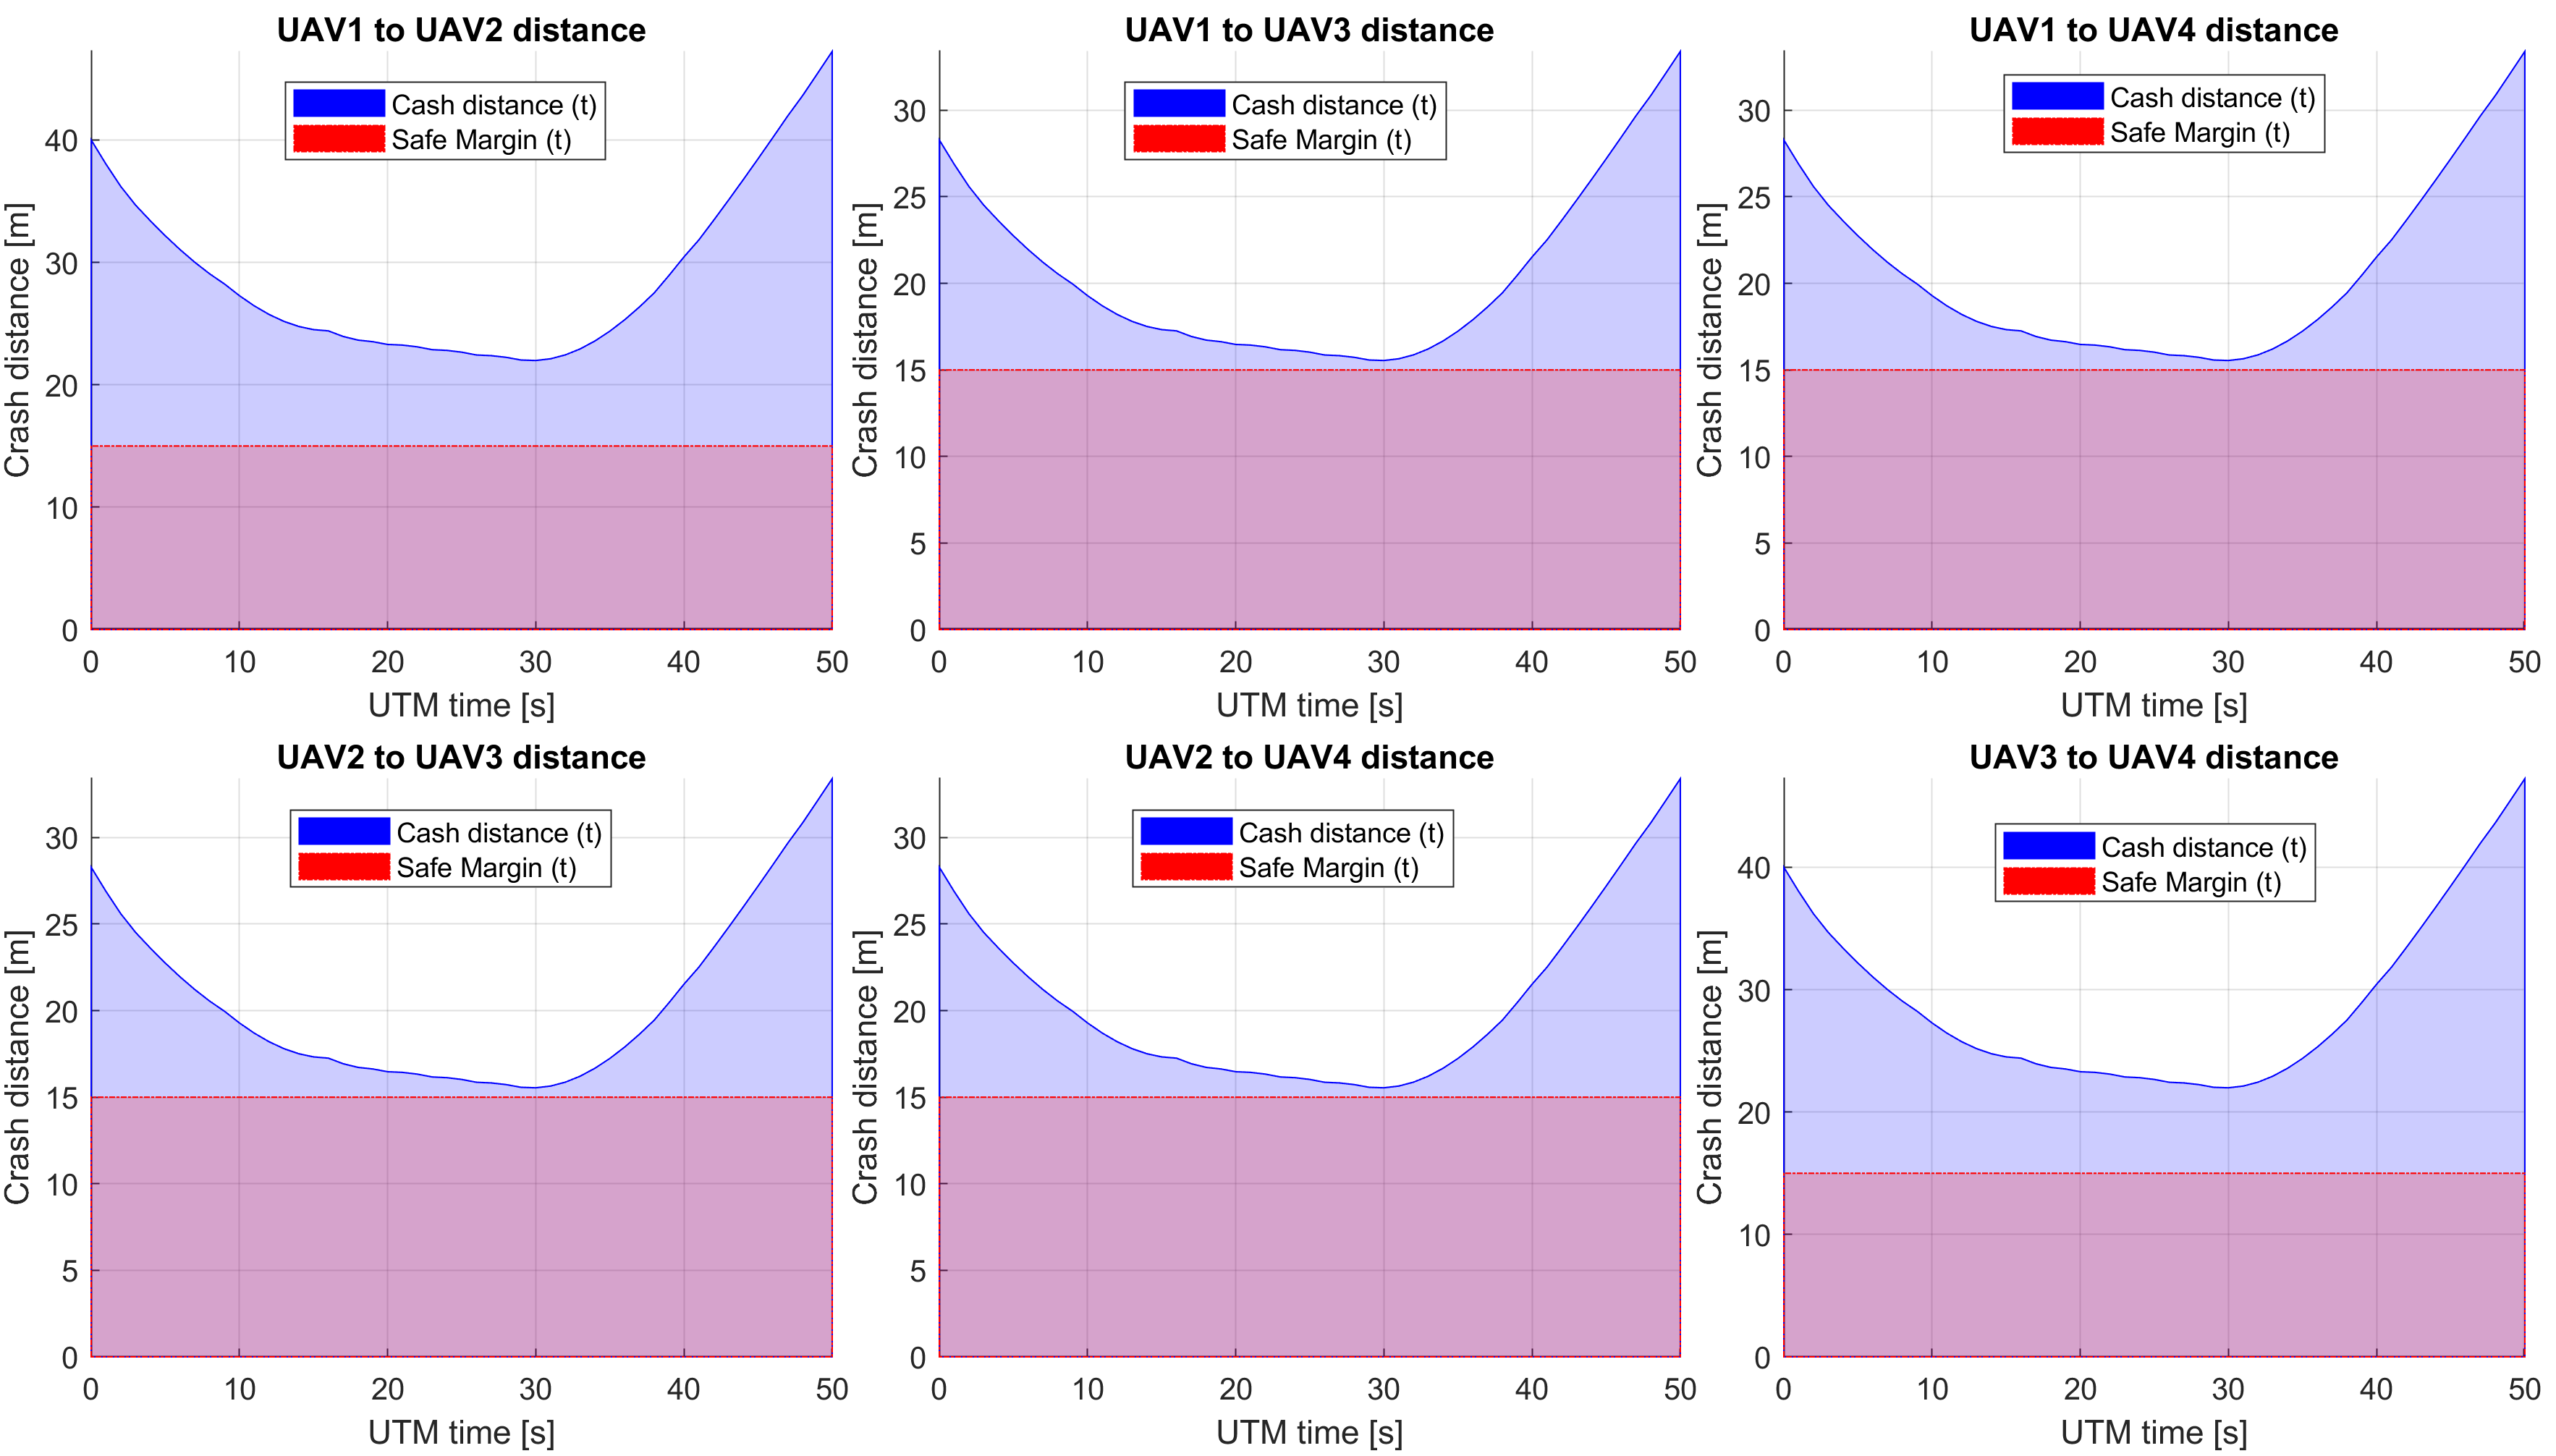
\includegraphics[width=0.9\linewidth]{\FIGDIR/NS066UtmCooperativeHeadOnMultiplePerformance}
	\caption{Distance to safety margin evolution for \emph{rule-based mixed scenario}.}
	\label{fig:testRuleBasedMultipleAvoidancePerformance}
\end{figure}

\paragraph{Distance to Safety Margin Peaks:} \emph{Distance to Safety Margin Peaks} (tab. \ref{tab:testCaseRuleBasedMixedSafetyMarginDistances}) represents the proximity of \emph{UAS mutual distance to breach well clear condition}. The \emph{breach condition} was not fulfilled in any combination. 

The \emph{minimal distance to safety margin} was $0.5438$ $m$ between all four \emph{UAS} systems. The \emph{maximal distance to safety margin} ranges between \emph{18 - 32 m} which show advantages of the \emph{virtual roundabout}.

\begin{table}[H]
	\centering
	\begin{tabular}{c||c|c|c}
		\multirow{2}{*}{UAS:} & \multicolumn{3}{c}{Distance to Safety Margin} \\ \cline{2-4} 
				  & min          & max         & breach         \\ \hline\hline
			1-2   & 6.9823       & 32.2369     & false          \\ \hline
			1-3   & 0.5438       & 18.4015     & false          \\ \hline
			1-4   & 0.5438       & 18.4015     & false          \\ \hline
			2-3   & 0.5438       & 18.4015     & false          \\ \hline
			2-4   & 0.5438       & 18.4015     & false          \\ \hline
			3-4   & 6.9823       & 32.2369     & false          \\ 
	\end{tabular}
	\caption{Distance to safety margin peaks for \emph{rule-based mixed scenario}.}
	\label{tab:testCaseRuleBasedMixedSafetyMarginDistances}
\end{table}


\paragraph{Path Tracking Performance:} Path tracking is displayed in (fig. \ref{fig:testCaseRuleBasedMixedTrajectoryTracking}). The UAS trajectory is divided into \emph{X, Y, Z axis tracking over UTM Time}. The \emph{Reference Trajectory} (green dashed line) is represented as the interconnection between \emph{Start Waypoint} (green square marked S) and  \emph{Goal Waypoint $\mathscr{WP}_1$} (green square marked 1). The \emph{Executed trajectory} (solid blue  line) reflects real \emph{UAS} movement.

\begin{enumerate}
	\item \emph{UAS 1} (fig. \ref{fig:ruleBasedMixedPathTrackingUAS1}) is using the bottom portion of \emph{Virtual Roundabout} (-Y values), sticking to the boundary of the \emph{Virtual Roundabout}.
	
	\item \emph{UAS 2} (fig. \ref{fig:ruleBasedMixedPathTrackingUAS2}) is using the upper portion of the \emph{Virtual Roundabout}. (+Y values), sticking to the boundary of the \emph{Virtual Roundabout}.
	
	\item \emph{UAS 3} (fig. \ref{fig:ruleBasedMixedPathTrackingUAS3}) is using the right portion of the \emph{Virtual Roundabout}. (+X values), sticking to the boundary of the \emph{Virtual Roundabout}.
	
	\item \emph{UAS 4} (fig. \ref{fig:ruleBasedMixedPathTrackingUAS4}) is using the left portion of the \emph{Virtual Roundabout}. (-X values), sticking to the boundary of the \emph{Virtual Roundabout}.
\end{enumerate}

\begin{figure}[H]
	\centering
	\begin{subfigure}{0.48\textwidth}
		\centering
		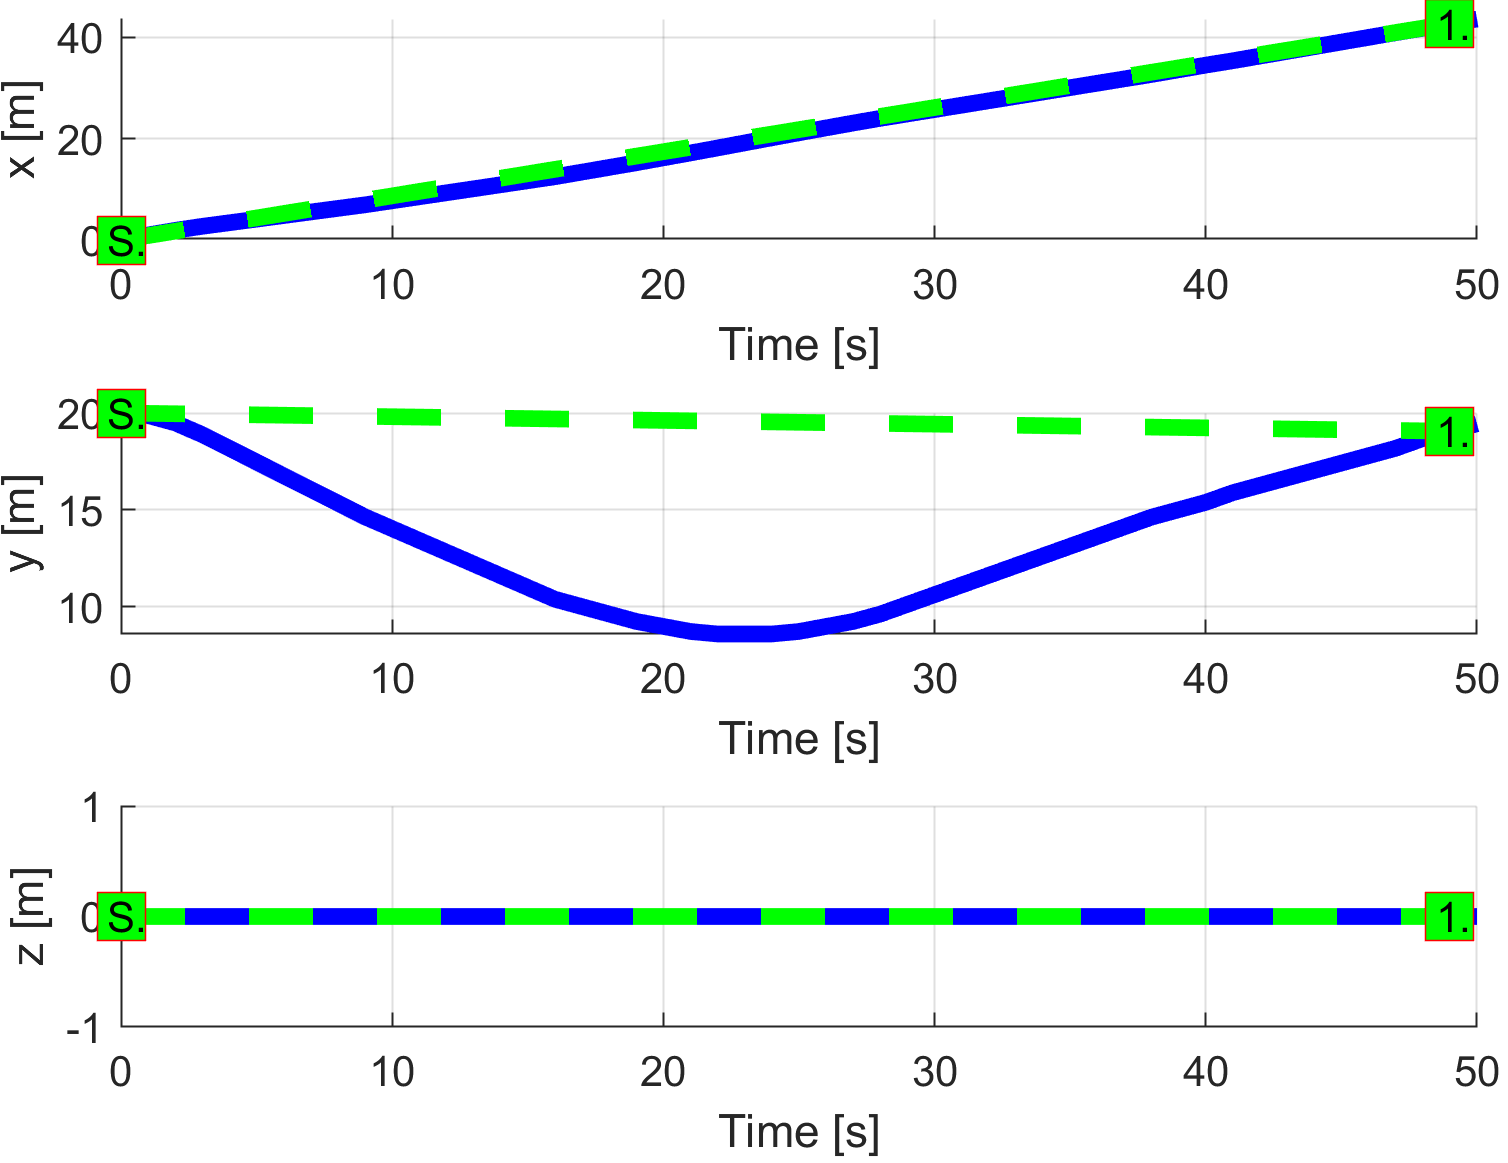
\includegraphics[width=0.9\linewidth]{\FIGDIR/NS067UtmCooperativeHeadOnMultipleUAV1PathFollowing}
		\caption{UAS 1.}
		\label{fig:ruleBasedMixedPathTrackingUAS1}
	\end{subfigure}
	\begin{subfigure}{0.48\textwidth}
		\centering
		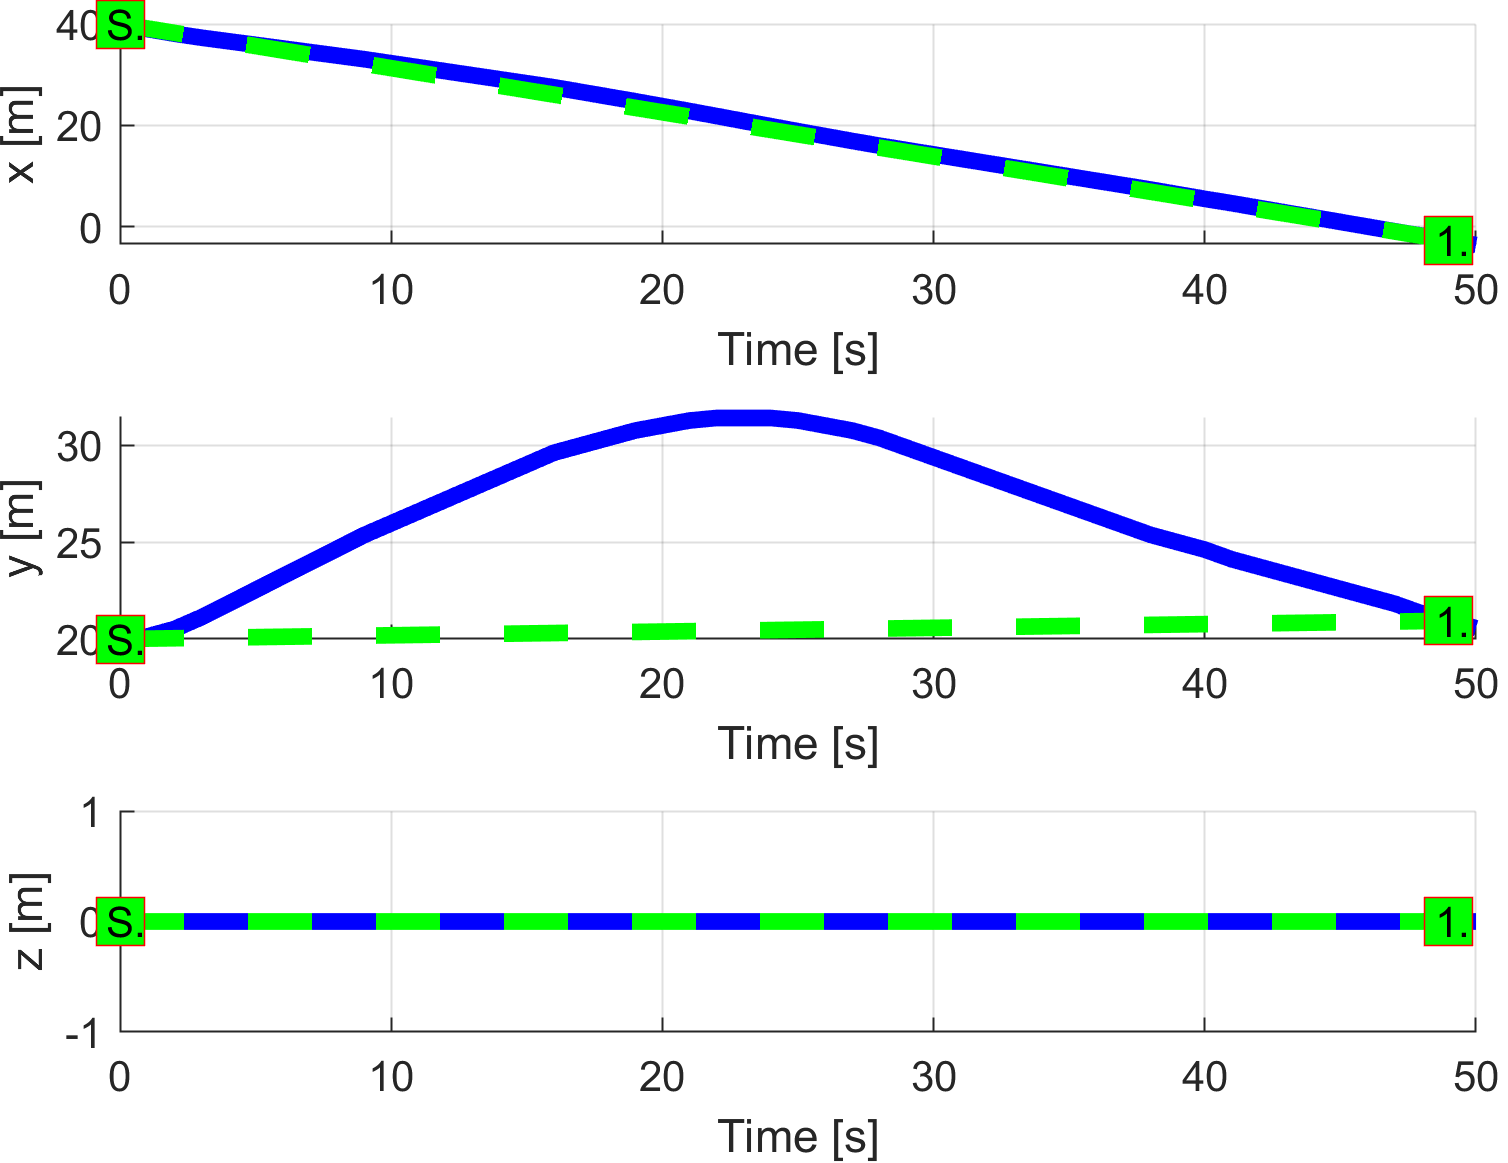
\includegraphics[width=0.9\linewidth]{\FIGDIR/NS068UtmCooperativeHeadOnMultipleUAV2PathFollowing} 
		\caption{UAS 2.}
		\label{fig:ruleBasedMixedPathTrackingUAS2}
	\end{subfigure}
	\\
	\begin{subfigure}{0.48\textwidth}
		\centering
		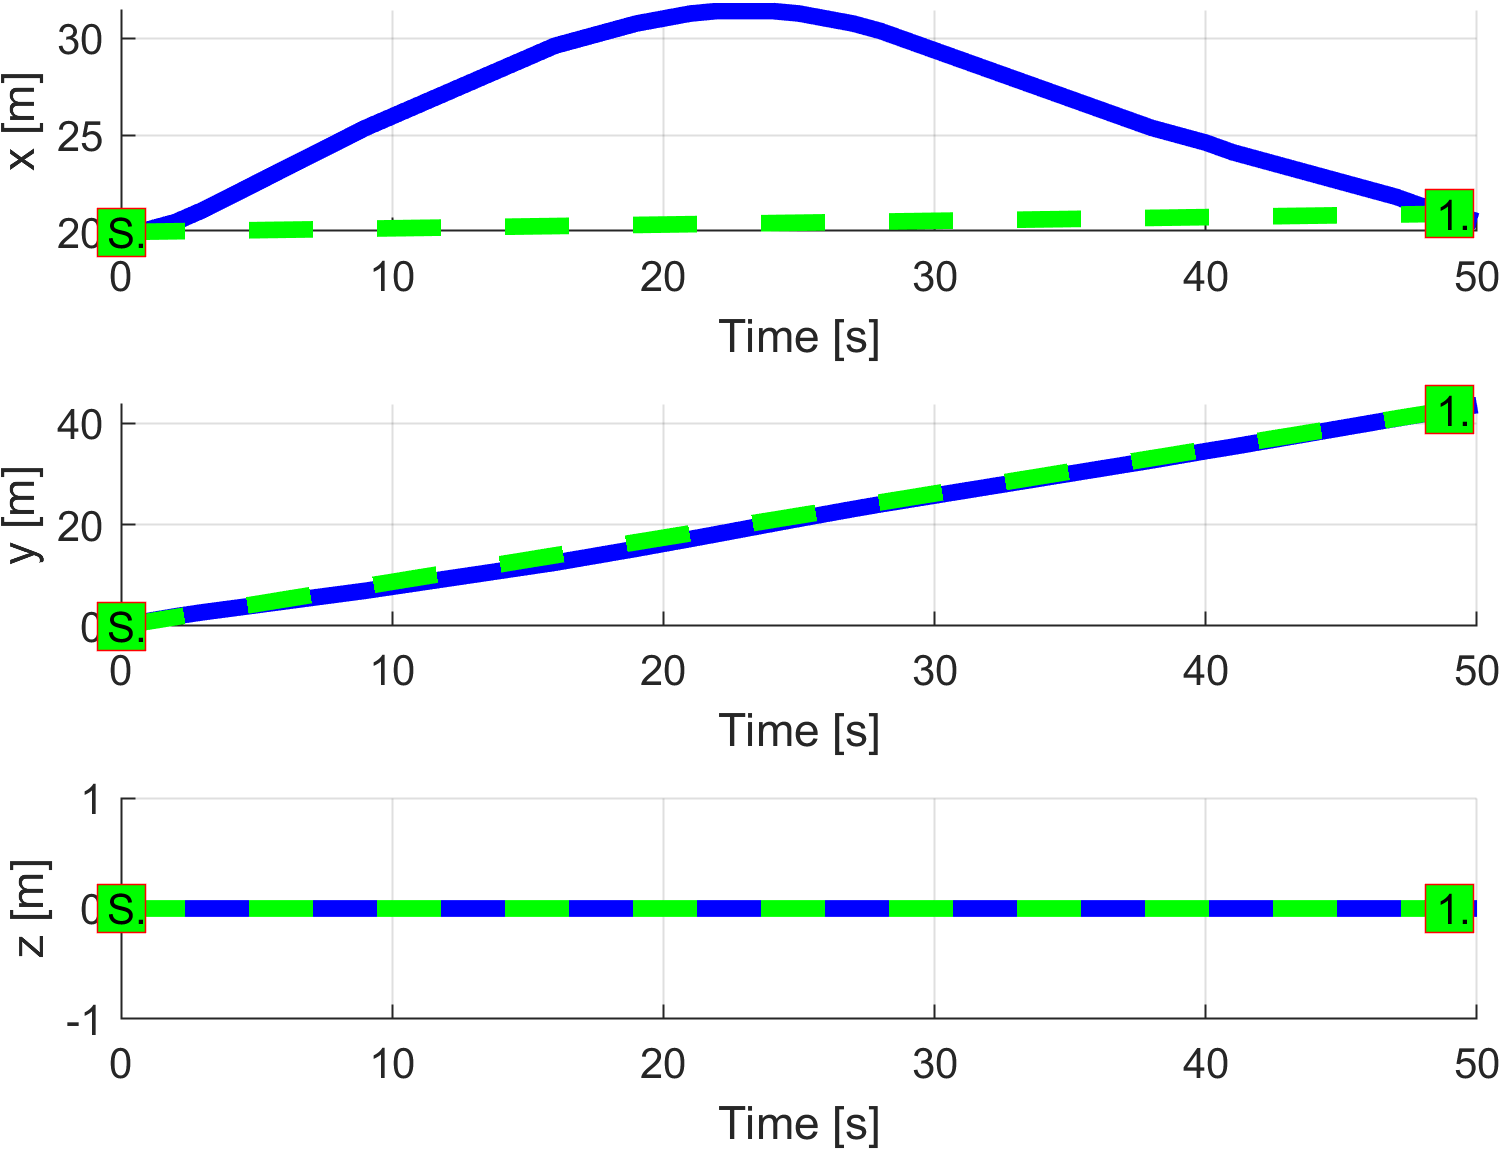
\includegraphics[width=0.9\linewidth]{\FIGDIR/NS069UtmCooperativeHeadOnMultipleUAV3PathFollowing} 
		\caption{UAS 3.}
		\label{fig:ruleBasedMixedPathTrackingUAS3}
	\end{subfigure}
	\begin{subfigure}{0.48\textwidth}
		\centering
		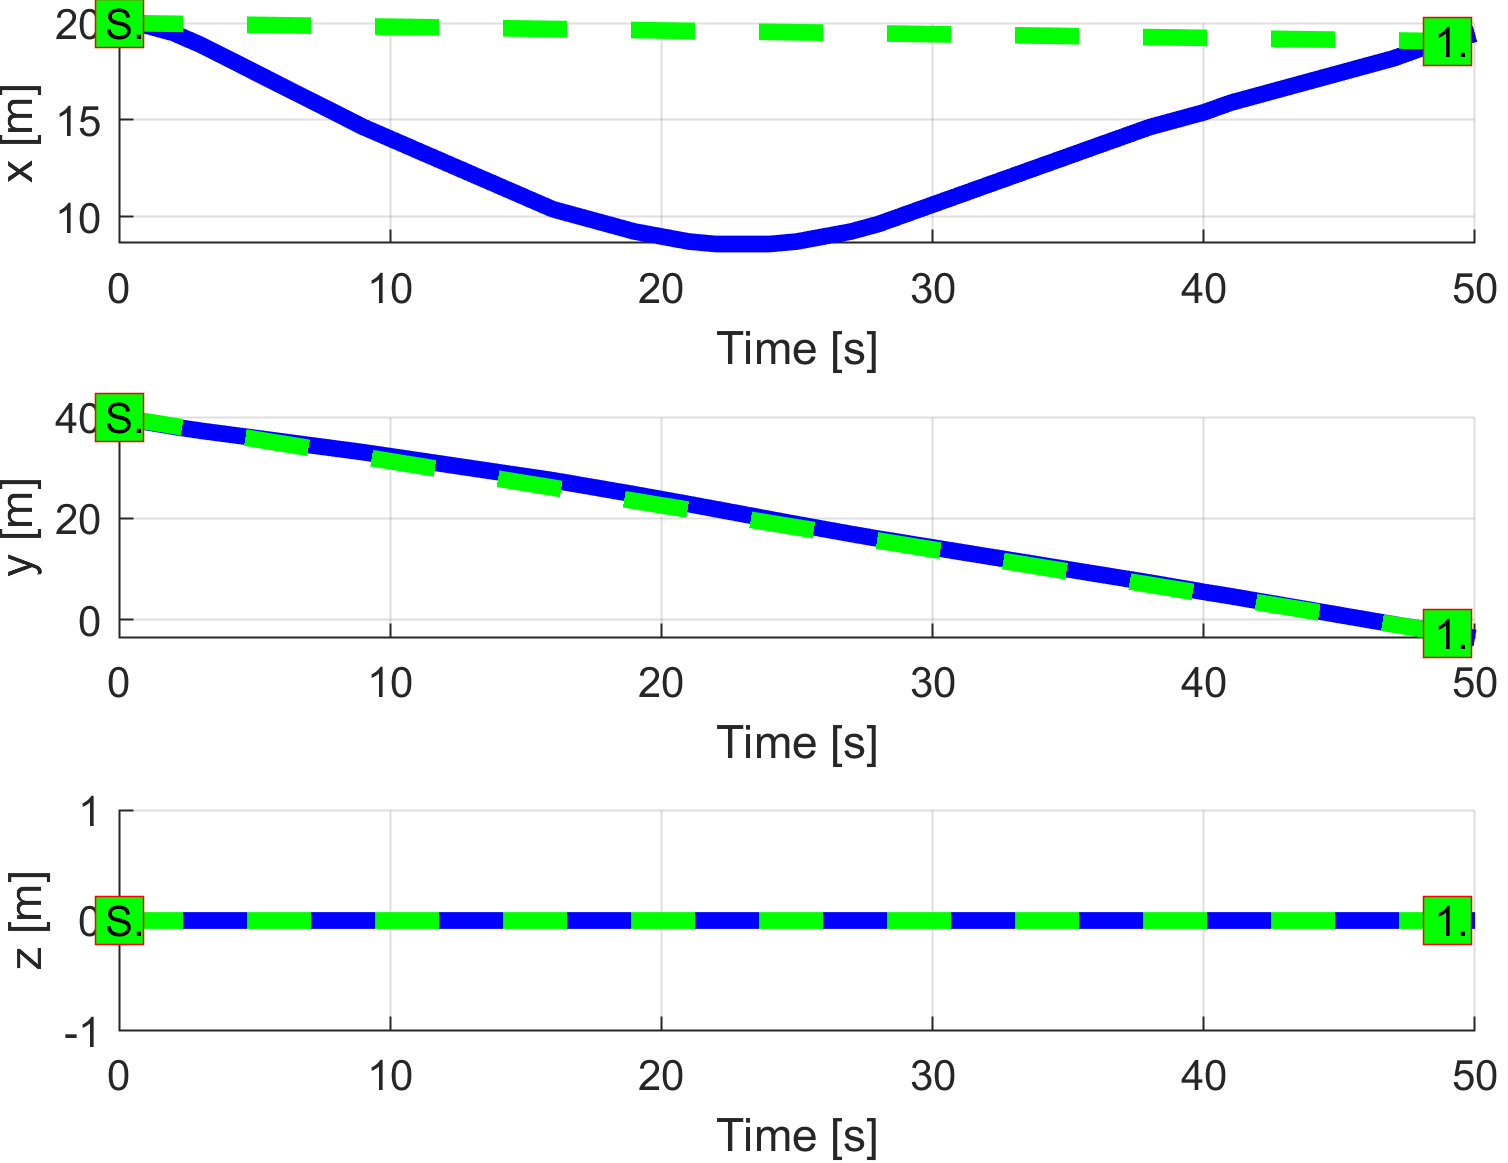
\includegraphics[width=0.9\linewidth]{\FIGDIR/NS070UtmCooperativeHeadOnMultipleUAV4PathFollowing} 
		\caption{UAS 4.}
		\label{fig:ruleBasedMixedPathTrackingUAS4}
	\end{subfigure}
	\caption{Trajectory tracking for \emph{rule-based mixed} situation test case.}
	\label{fig:testCaseRuleBasedMixedTrajectoryTracking}
\end{figure}

\newpage
\paragraph{Path Tracking Deviations:} \emph{Deviations} (tab. \ref{tab:pathTrackingParametersForRuleBasedMixed}) are in expected ranges, considering the mission plans (tab. \ref{tab:missionSetupRuleBasedMixedScenario}) and \emph{Merged Case Safety Margin} ($15$ $m$).

\begin{table}[H]
	\centering
	\begin{tabular}{c||c|c|c|c}
		\multirow{2}{*}{Param.} & UAS 1     & UAS 2             & UAS 3             & UAS 4 \\\cline{2-5}
						& $\mathscr{WP}_1$  & $\mathscr{WP}_1$  & $\mathscr{WP}_1$  & $\mathscr{WP}_1$ \\\hline\hline
		  $\max |x|$    & 0                 & 0                 & 11.40             & 11.40\\\hline
		  $\max |y|$    & 11.40             & 11.40             & 0                 & 0\\\hline
		  $\max |z|$    & 0                 & 0                 & 0                 & 0\\\hline
		  $\max dist.$  & 11.40             & 11.40             & 11.40              & 11.40\\
	\end{tabular}
	\caption{Path tracking properties for \emph{rule-based mixed} scenario.}
	\label{tab:pathTrackingParametersForRuleBasedMixed}
\end{table}


% 10 Rule Based Multiple
\paragraph{Computation Load:} The \emph{computation load} for \emph{scenario} (fig.\ref{fig:ruleBasedMultipleComputationTime}) shows used time (y-axis) over decision frame (x-axis).

The \emph{computation time} for each UAS has the same evolution. The \emph{load} is higher  during avoidance maneuver on the \emph{virtual roundabout}.

\begin{figure}[H]
\centering
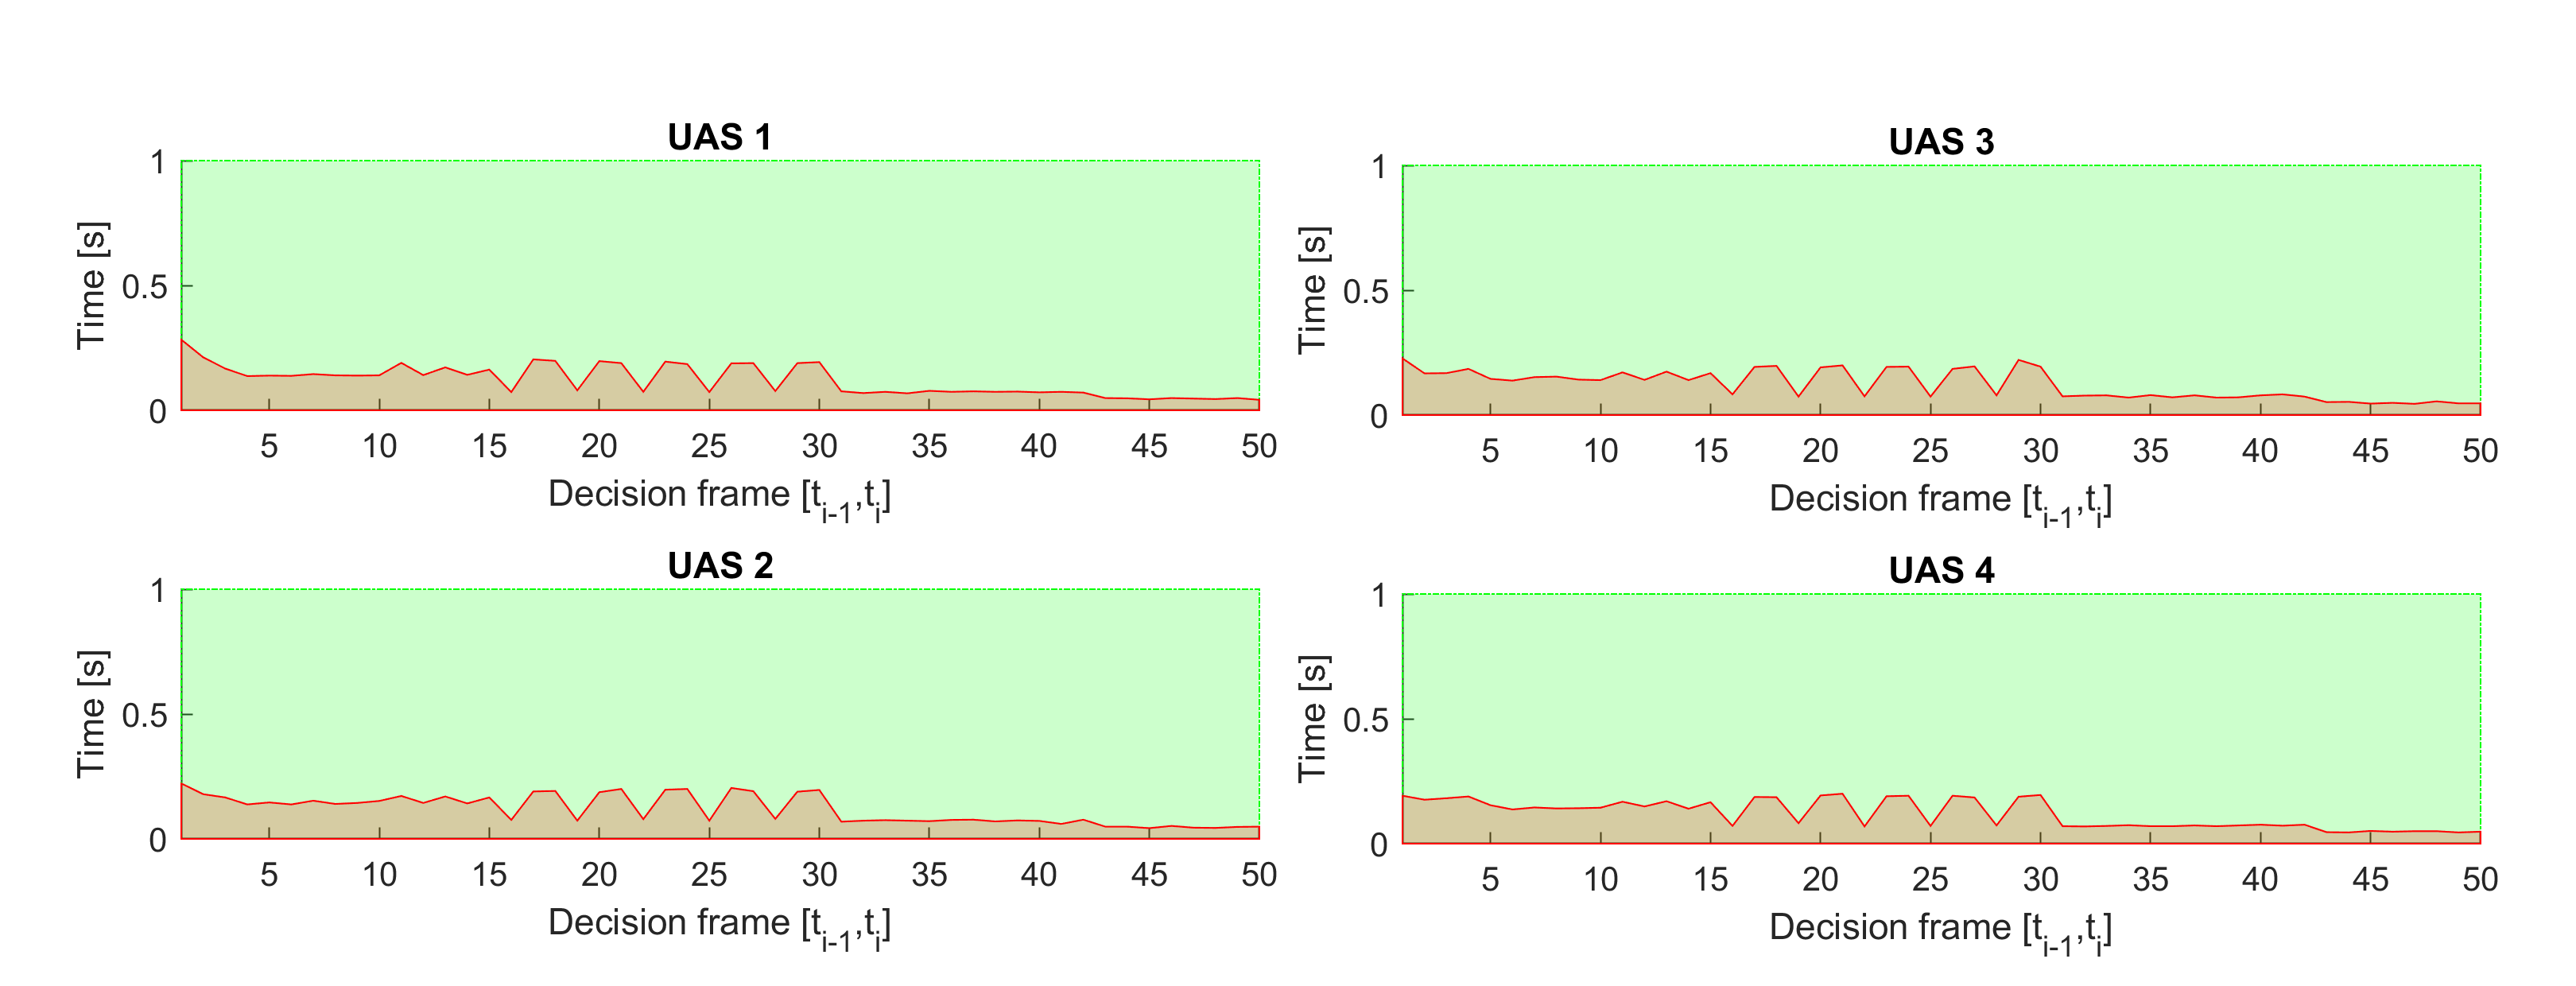
\includegraphics[width=0.95\linewidth]{\FIGDIR/NS101RuleBasedMultipleComputationTime} 
\caption{Computation time for \emph{rule-based multiple} scenario.}
\label{fig:ruleBasedMultipleComputationTime}
\end{figure}
    	\newpage
\subsection{Rule based Overtake}\label{s:testRuleOvertake}
    \paragraph{Scenario:} Two UAS are flying in the \emph{controlled airspace} (over 500 feet Above Ground Level) on the \emph{airway} (in same direction). \emph{Slower UAS} is in front of \emph{Faster UAS}. There is possibility of a \emph{collision} or a \emph{near miss incident} or a \emph{well clear breach}. The \emph{Faster UAS} (Overtaking) must contact \emph{UTM} service and ask for \emph{overtake permission}. Scenario steps:
    
    \begin{enumerate}
        \item \emph{Faster UAS} (Overtaking) notices \emph{UTM} service about \emph{Slower UAS} (Overtaken). (This step is Optional.)
        
        \item \emph{UTM} service issues \emph{Directives} to all \emph{UAS} in area.
        
        \item \emph{Overtake Directive} is received by \emph{Faster UAS} (Overtaking) and \emph{Slower UAS} (Overtaken).
        
        \item \emph{Faster UAS} (Overtaking) mission plan is altered to reflect \emph{Overtake directive}, \emph{Divergence Waypoint} and \emph{Convergence Waypoint} are added.
        
        \item \emph{Faster UAS} (Overtaking) safely overtakes \emph{Slower UAS} (Overtaken) without breaking \emph{Well clear} condition.
    \end{enumerate}
    
    \noindent\emph{Mission parameters} for both \emph{UAS} systems are defined in (tab. \ref{tab:missionSetupRuleBasedOvertakeScenarios}).
    
    \begin{table}[H]
        \centering
        \begin{tabular}{c||c|c||c}
            \multirow{2}{*}{UAS} &\multicolumn{2}{c||}{Position} & \multirow{2}{*}{$\mathscr{WP}_1$} \\\cline{2-3}
              & $[x,y,z]$           & $[\theta,\varpi,\psi]$           & \\\hline\hline
            1 & $[-40,20,0]^T $       & $[0^\circ,0^\circ,0^\circ]^T$    & $[110,20,0]^T$\\\hline 
            2 & $[-20,20,0]^T $       & $[0^\circ,0^\circ,0^\circ]^T$    & $[80,20,0]^T$\\
        \end{tabular}
        \caption{Mission setup for all \emph{Rule based overtake} scenarios.}
        \label{tab:missionSetupRuleBasedOvertakeScenarios}
    \end{table}


    \paragraph{Assumptions:} Following assumptions are valid for this test:
    
    \begin{enumerate}
        \item \emph{Controlled Airspace Airworthiness} - UAS system is equipped with necessary controlled airspace equipment like ADS-B In/Out, Radar, Transponder, etc. Moreover airworthy \emph{UAS} has capability to precisely follow \emph{UTM directives} (max. 5 $\%$ deviation).
        
        \item \emph{C2 (Command \& control) Link Established} - necessary for (UAS $\leftrightarrow$ UAS) and (UAS $\leftrightarrow$ UTM) communication. If \emph{C2} link is lost the \emph{UAS} will enter into \emph{Emergency avoidance mode}.
        
        \item \emph{Decision frame synchronization with UTM} - necessary in discrete C2 environment otherwise \emph{safety margins} needs to be \emph{bloated}.
    \end{enumerate}
    
    \paragraph{Main Goal:} Show possibility of \emph{Overtake Maneuver} invoked by the \emph{UTM Directive} (event based flight constraint). 
    
    \paragraph{Acceptance Criteria:} Following criteria must be met:
    \begin{enumerate}
        \item \emph{Proper passing of Divergence/Convergence Waypoint} - minimal distance of \emph{UAS trajectory} to \emph{Divergence/Convergence waypoint} must be below passing threshold. Waypoints needs to be passed in given order (Divergence $1^{st}$, Convergence $2^{nd}$).
        
        \item \emph{Slower UAS (Overtaken) keeps Right of the Way} - the UAS with lesser maneuverability does not stand a chance in avoidance situation, it needs to keep its \emph{Right of the Way}. 
        
        \item \emph{Both UAS does not breach Well Clear (safety) Margin} - mutual distance does not get trough \emph{calculated Safety Margin}.
    \end{enumerate}
    
    \paragraph{Testing Setup:} The \emph{standard test setup} for each UAS defined in (tab. \ref{tab:testMovementOrientations}, \ref{tab:testUASBasicParameters}, \ref{tab:testNavigationGridBasic}, \ref{tab:testAvoidanceGridBasic}, \ref{tab:testUASColoring}) is used with following parameter override:
    \begin{enumerate}
        \item \emph{Navigation grid - type} - \emph{ACAS-like} with enabled \emph{Horizontal maneuvers}
    \end{enumerate}
    
    This \emph{configuration} is based on assumption that every UAS is in \emph{controlled airspace} in \emph{FL450} (flight level 45000 feet Above Sea Level), without permission for \emph{climb or descent maneuver}. \emph{Rule engine} is initialized in standard \emph{Rules of the air} configuration (fig. \ref{fig:RuleEngineInstanceLevels}).
    
    There is \emph{UTM} service for given \emph{airspace cluster} calculating \emph{collision cases} (tab. \ref{tab:collisionCase}) based on incoming \emph{UAS position notifications} (tab. \ref{tab:positionNotification}).
    
    
    \paragraph{Simulation Run:} Notable moments from the \emph{simulation run} (fig. \ref{fig:testCaseRuleBasedOvertake2xSpeed}) are following:
    
    \begin{enumerate}
        \item \emph{Collision case creation} (fig.\ref{fig:ruleBasedOvertake2xCollisionCaseCreation}) - \emph{Faster UAS} (blue) receives \emph{UTM Directive} to invoke \emph{Overtake Rule} (tab. \ref{tab:ruleOvertakeDefinition}). \emph{Slower UAS} (magenta) receives \emph{UTM Directive} to keep \emph{Right of the Way} and warning that is going to be \emph{Overtaken}. \emph{Faster UAS} (blue) creates two \emph{virtual waypoints}:
        \begin{enumerate}[a.]
            \item \emph{Divergence waypoint} at position $[0,14,0]^T$.
            \item \emph{Convergence waypoint} at position $[24,14,0]^T$.
        \end{enumerate}
        \emph{Faster UAS} then sets \emph{Divergence waypoint} as \emph{Goal waypoint} and It starts overtake maneuver while checking mutual distance.
        
        \item \emph{Divergence waypoint reach} (fig. \ref{fig:ruleBasedOvertake2xDivergenceWaypointReach}) - \emph{Faster UAS} (blue) successfully reached \emph{Divergence Waypoint}, setting \emph{Convergence Waypoint} as new \emph{Goal waypoint}.
        
        \item \emph{Convergence waypoint reach} (fig. \ref{fig:ruleBasedOvertake2xConvergenceWaypointReach}) - \emph{Faster UAS} (blue) successfully reached \emph{Convergence Waypoint}, setting \emph{Original Goal Waypoint} as new \emph{Goal waypoint}. The \emph{UTM} service is notified from \emph{Faster UAS} (blue) that \emph{Overtaken Maneuver} have been completed. UTM \emph{acknowledges} maneuver competition and It sends notification to \emph{Slower UAS} (magenta) that \emph{Overtake Maneuver} is finished. \emph{Slower UAS} (magenta) was successfully overtaken.
        
        \item \emph{Original waypoint reach} (fig. \ref{fig:ruleBasedOvertake2xOriginalWaypointReach}) - \emph{Faster UAS} (blue) successfully reached \emph{Original Waypoint}, Starting landing Sequence. 
    \end{enumerate}


    \begin{figure}[H]
        \centering
        \begin{subfigure}{0.75\textwidth}
            \centering
            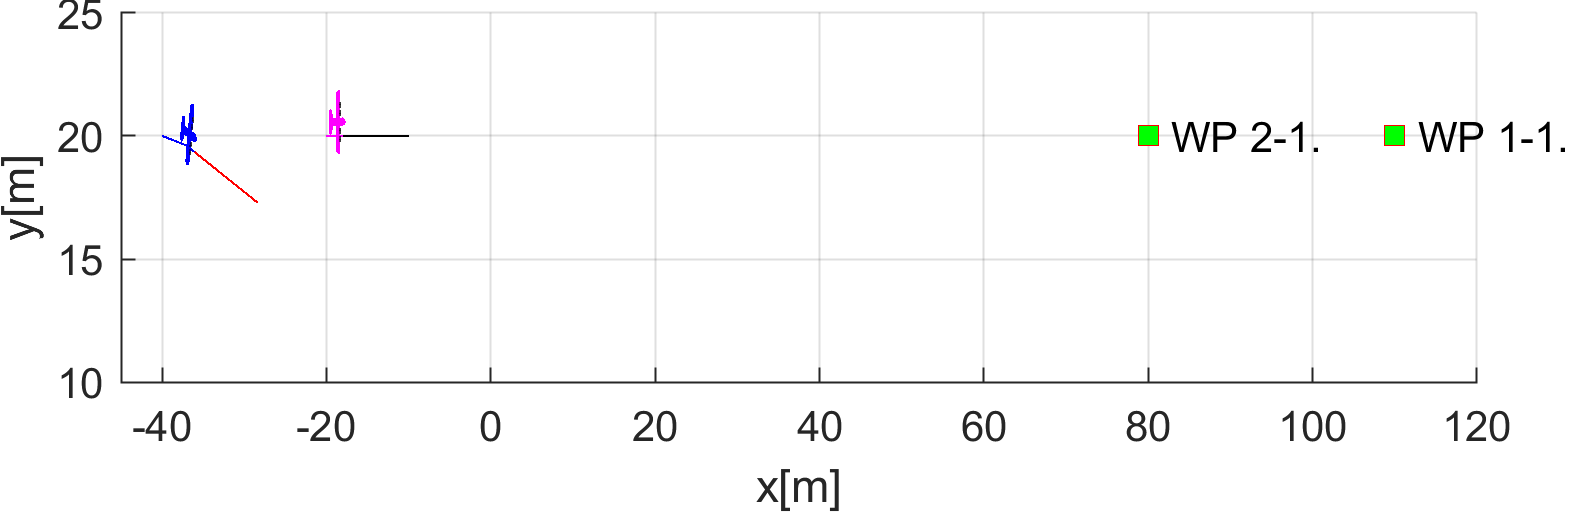
\includegraphics[width=0.9\linewidth]{\FIGDIR/NS071UtmCooperativeOvertake2xSpeed00002}
            \caption{Collision case creation.}
            \label{fig:ruleBasedOvertake2xCollisionCaseCreation}
        \end{subfigure}
        \\
        \begin{subfigure}{0.75\textwidth}
            \centering
            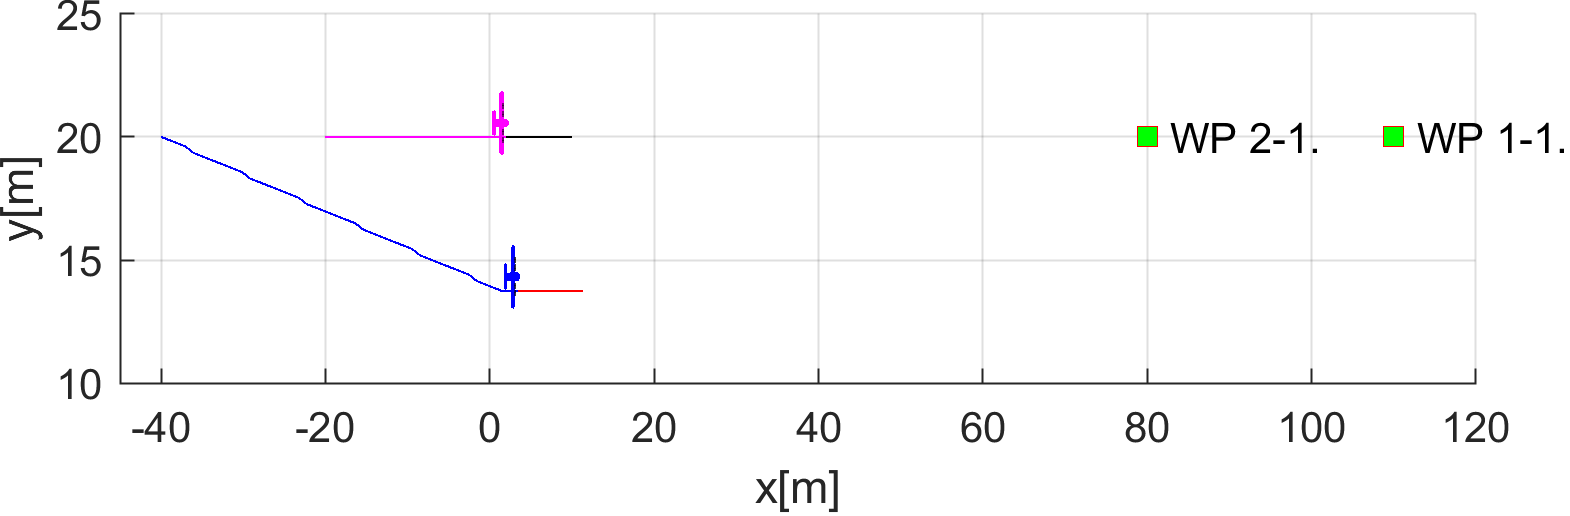
\includegraphics[width=0.9\linewidth]{\FIGDIR/NS072UtmCooperativeOvertake2xSpeed00022} 
            \caption{Divergence waypoint reach.}
            \label{fig:ruleBasedOvertake2xDivergenceWaypointReach}
        \end{subfigure}
        \\
        \begin{subfigure}{0.75\textwidth}
            \centering
            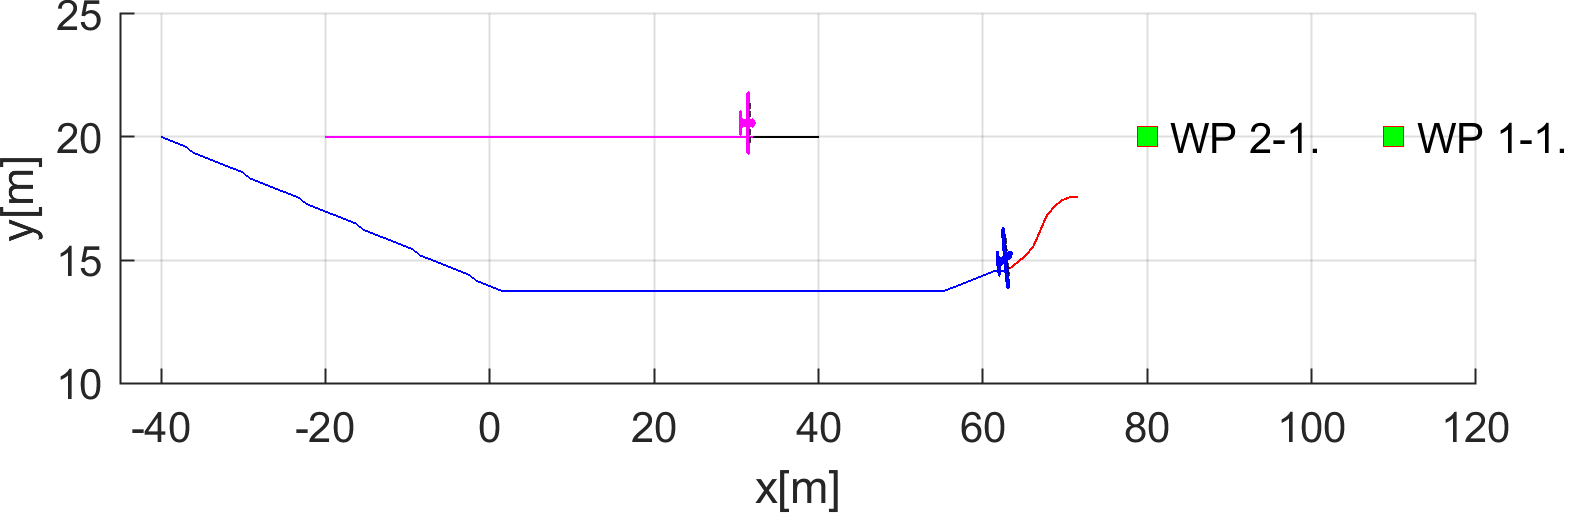
\includegraphics[width=0.9\linewidth]{\FIGDIR/NS073UtmCooperativeOvertake2xSpeed00052} 
            \caption{Convergence waypoint reach.}
            \label{fig:ruleBasedOvertake2xConvergenceWaypointReach}
        \end{subfigure}
        \\
        \begin{subfigure}{0.75\textwidth}
            \centering
            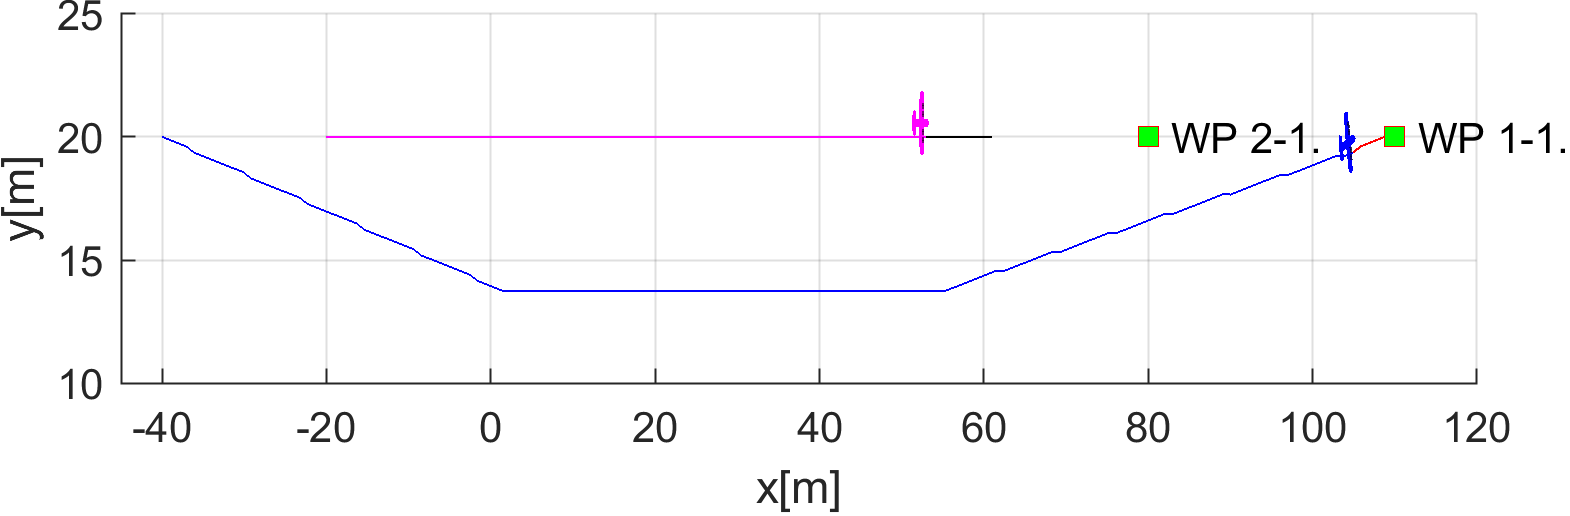
\includegraphics[width=0.9\linewidth]{\FIGDIR/NS074UtmCooperativeOvertake2xSpeed00073} 
            \caption{Original waypoint reach.}
            \label{fig:ruleBasedOvertake2xOriginalWaypointReach}
        \end{subfigure}
        \caption{Test scenario for \emph{Rule based Overtake} (double speed of overtaking aircraft). }
        \label{fig:testCaseRuleBasedOvertake2xSpeed}
    \end{figure}
    

    \paragraph{Collision Case Calculation:} The \emph{Collision Case} (tab. \ref{tab:collisionCasesRuleOvertake2x}) was calculated according to \emph{Collision Calculation process} (sec. \ref{sec:collisionCase}). \emph{Faster UAS} (1) has \emph{Overtaking} role and \emph{Slower UAS} has \emph{Right of the Way}. \emph{Collision Point} is direct type at $[0.20.0]^T$. \emph{Collision case type} was set based on \emph{angle of approach} $0^{\circ}$ as \emph{Overtake}. The \emph{Safety Margin} was set as \emph{5 m}.
    
    
    \begin{table}[H]
        \centering
        \begin{tabular}{c|c|c|c|c|c||c|c}
            \multicolumn{6}{c||}{Collision Case}& \multicolumn{2}{c}{Margins} \\ \hline
            id  & UAS & role & \begin{tabular}[c]{@{}c@{}}collision\\ point\end{tabular} & \begin{tabular}[c]{@{}c@{}}angle of\\ approach\end{tabular} & type&  safety  & case  \\ \hline\hline
            % Case 1-2
            \multirow{2}{*}{1-2} & 1   & Overtaking & \multirow{2}{*}{$[0,20,0]^T$} & \multirow{2}{*}{$0^\circ$} & \multirow{2}{*}{Overtake} & 5 & \multirow{2}{*}{5} \\ \cline{2-3} \cline{7-7} & 2   & Right o.W. & & & & 5& \\ 
        \end{tabular}
        \caption{Collision case for \emph{Rule-based Overtake} scenario 2x speed.}
        \label{tab:collisionCasesRuleOvertake2x}
    \end{table}
    
    
    \paragraph{Overtake Speed: Divergence/Convergence Waypoints}
    \emph{Divergence waypoints} have been calculated according to (eq. \ref{eq:overtakeDivergenceLocal}), and, \emph{Convergence Waypoints} have been calculated according to (eq. \ref{eq:overtakeConvergenceLocal}). Following \emph{Speed Differences} were taken into account (Faster/Slower UAS speed ratio): \emph{2x, 3x, 4x}. Following observations can be made:
    
    \begin{enumerate}
        \item \emph{Distance between Divergence and Convergence waypoint} is decreasing with increasing \emph{speed difference}.
        
        \item \emph{Divergence waypoint} is moving \emph{back/right} in \emph{UAS Local Coordinate Frame} with Increasing \emph{speed difference}. 
        
        \item \emph{Convergence waypoint} is moving like \emph{Divergence waypoint} but little bit faster.
    \end{enumerate}
    
    \begin{table}[H]
        \centering
        \begin{tabular}{c||c|c||c|c||c}
            %Header line 1
            \multirow{2}{*}{\begin{tabular}[c]{@{}c@{}}Speed\\ diff.\end{tabular}} & \multicolumn{2}{c||}{Divergence} & \multicolumn{2}{c||}{Convergence} & \multirow{2}{*}{\begin{tabular}[c]{@{}c@{}}Final\\ waypoint\end{tabular}} \\ \cline{2-5}
            %Header line 2
            & waypoint & \multirow{2}{*}{difference} & waypoint & \multirow{2}{*}{difference}  & \\ \cline{1-2} \cline{4-4} \cline{6-6} 
            % 2x speed 
            \multirow{2}{*}{2x} & \multirow{2}{*}{$[0,14,0]^T$} & & \multirow{2}{*}{$[24,14,0]^T$} & & \multirow{2}{*}{$[110,20,0]^T$} \\ \cline{3-3} \cline{5-5} 
            %  2-3 diff
            & & \multirow{2}{*}{$[-10,-1,0]^T$} & & \multirow{2}{*}{$[-8,-1,0]^T$} & \\ \cline{1-2} \cline{4-4} \cline{6-6} 
            % 3x speed
            \multirow{2}{*}{3x} & \multirow{2}{*}{$[-10,13,0]^T$} & & \multirow{2}{*}{$[16,13,0]^T$} & & \multirow{2}{*}{$[110,20,0]^T$} \\ \cline{3-3} \cline{5-5}
            % 3-4 diff
            & & \multirow{2}{*}{$[-3.4,-1,0]^T$} & & \multirow{2}{*}{$[-1.3,-1,0]^T$} & \\ \cline{1-2} \cline{4-4} \cline{6-6} 
            % 4x speed
            \multirow{2}{*}{4x} & \multirow{2}{*}{$[-13.4,12,0]^T$} & & \multirow{2}{*}{$[14.7,12,0]^T$} & & \multirow{2}{*}{$[110,20,0]^T$} \\ \cline{3-3} \cline{5-5}
            %filler line
            & & & & & \\ 
            \end{tabular}
        \caption{Convergence and divergence waypoints for various speed differences.}
        \label{tab:convergenceDivergenceWaypointsOvertake}
    \end{table}
    
    \paragraph{Overtake Speed: Impact on Trajectory} Overtake \emph{speed difference} is visible in (fig. \ref{fig:testCaseRuleBasedOvertakeDifferentSpeedTrajectoriesPerformance}). The \emph{Slower vehicle trajectory}(cyan) is following \emph{standard mission waypoints}. The \emph{Faster vehicle trajectory} for 2x (blue), 3x (green), 4x (black) are following \emph{Divergence/Convergence} waypoints from (tab. \ref{tab:convergenceDivergenceWaypointsOvertake}).
    
    \begin{figure}[H]
        \centering
        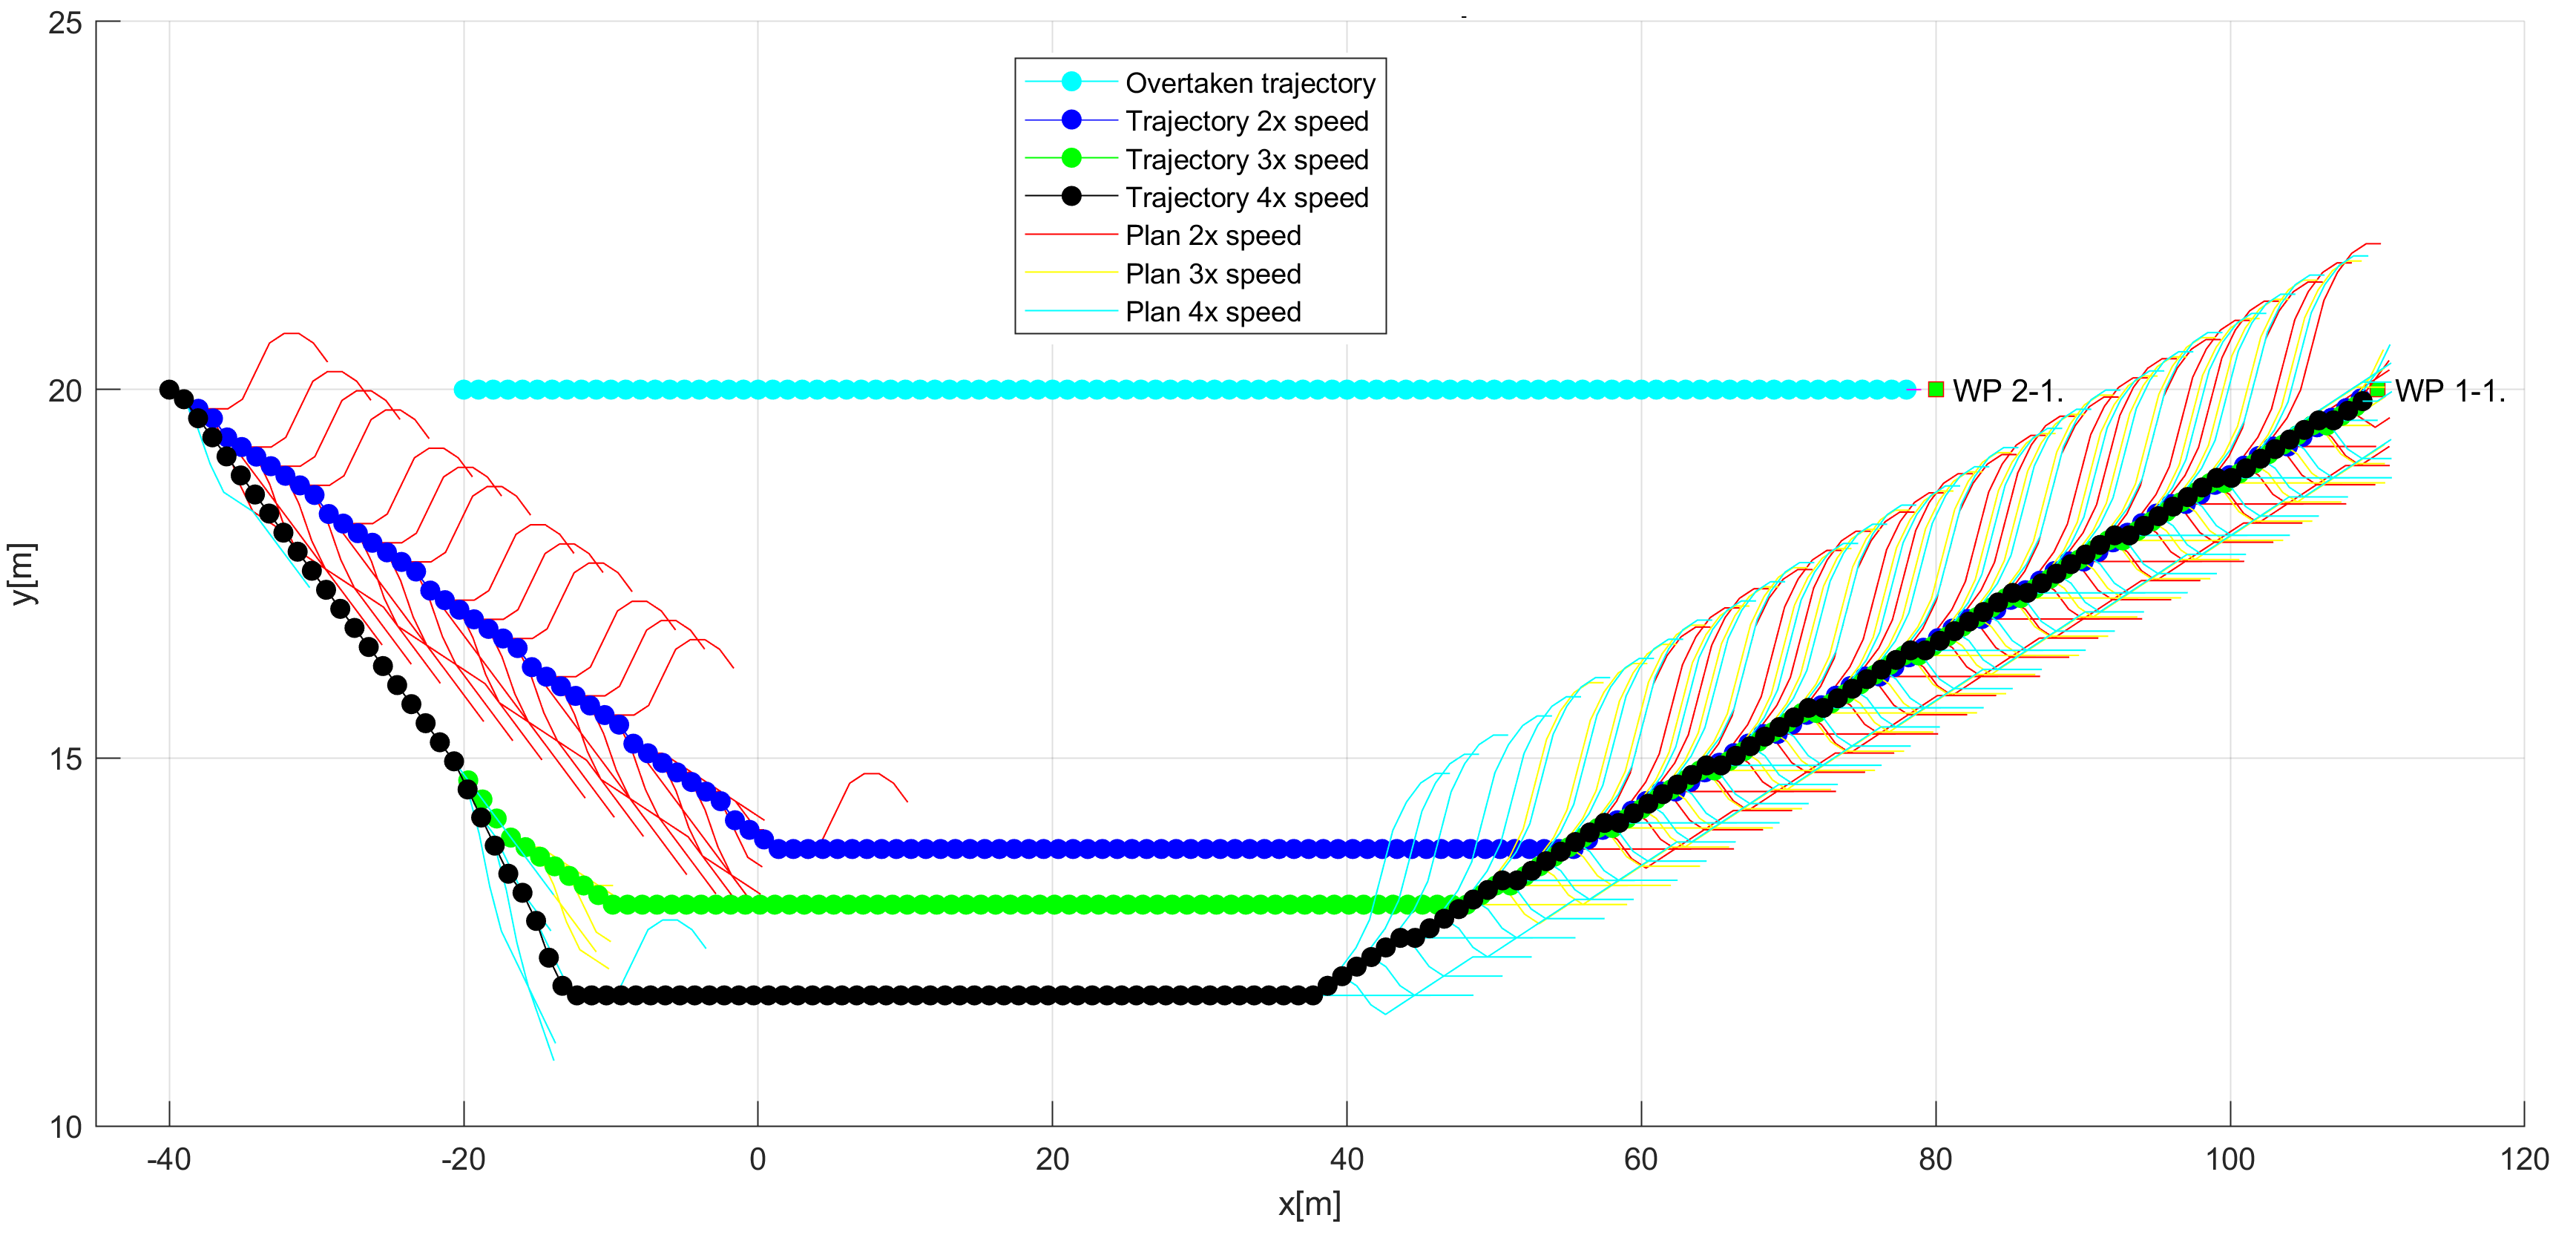
\includegraphics[width=0.9\linewidth]{\FIGDIR/NS078UtmCooperativeOvertakeMultipleTrajectories}
        \caption{\emph{Rule based overtake} trajectories for different speed.}
        \label{fig:testCaseRuleBasedOvertakeDifferentSpeedTrajectoriesPerformance}
    \end{figure}
    \newpage
    \paragraph{Overtake Speed: Impact on Distance to Safety Margin Evolution} \emph{Safety margin} (red line) is set to \emph{5 m}. It is obvious that \emph{Faster UAS} will take down \emph{Slower UAS} if there was not for an \emph{Overtake maneuver}.  The distance of \emph{Faster UAS} to \emph{Slower UAS} evolution is depending on \emph{Speed difference}. \emph{Inflection point} (closest point of two UAS) is reached sooner with \emph{Higher speed}. \emph{Safety margin performance} was measured for the \emph{UTM performance time} in interval $[0,35]$ $s$ and \emph{Speed difference} of 2x (blue), 3x (green), 4x (black).
    
    \begin{figure}[H]
        \centering
        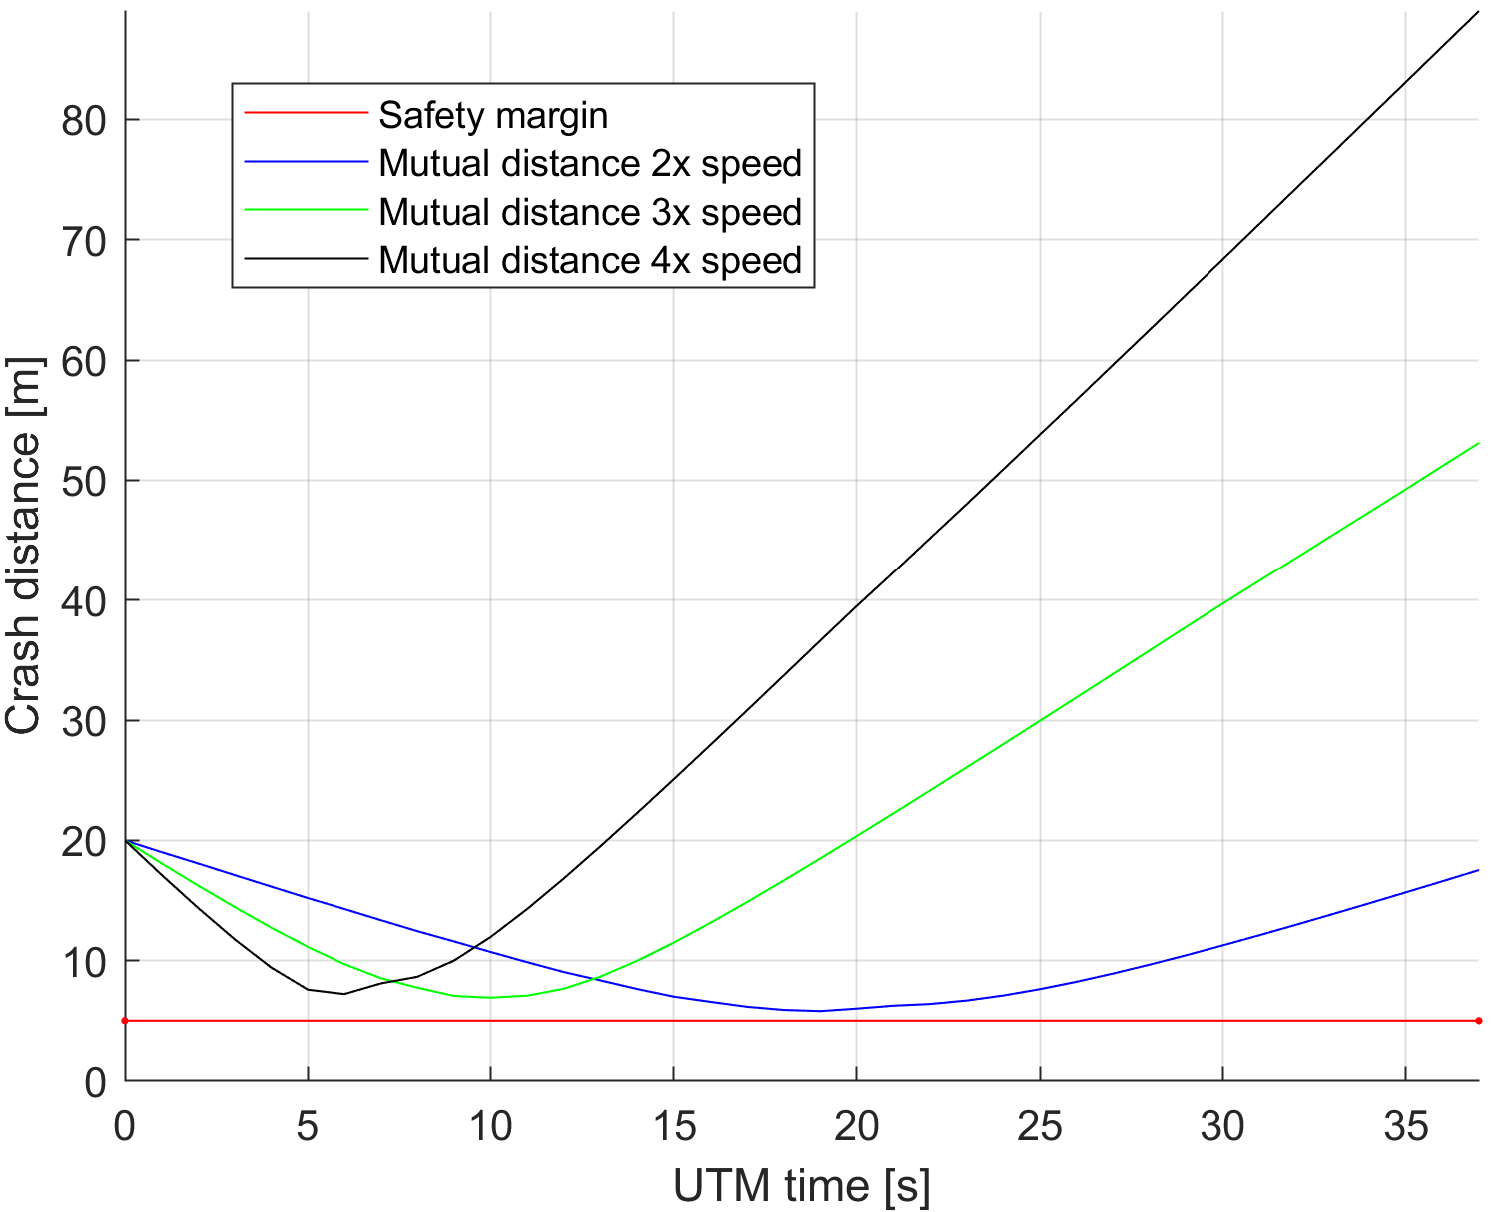
\includegraphics[width=0.6\linewidth]{\FIGDIR/NS079UtmCooperativeOvertakeMultiplePerformance}
        \caption{Overtake speed dependent distance to safety margin evolution for \emph{rule based overtake scenario}.}
        \label{fig:testRuleBasedOvertakeSafetyMarginForDifferentSpeedPerformance}
    \end{figure}
    
    \paragraph{Overtake Speed: Impact on Distance to Safety Margin Peaks} There is summary table (tab. \ref{tab:testCaseRuleBasedOvertakeSafetyMarginDistancesTimes}) for  measurement of minimal and maximal values for \emph{Distance to Safety Margin} over \emph{UTM time} (fig.\ref{fig:testRuleBasedOvertakeSafetyMarginForDifferentSpeedPerformance}). The minimal \emph{Overtake Distance to Safety Margin} in $0.7991$ $m$ for 2x \emph{Speed Difference}. The minimal \emph{Overtake closest point reach time} is $7$ $s$ for 4x \emph{Speed Difference}.
    
    For each \emph{Speed difference} (2x, 3x, 4x), the \emph{Well Clear Margin} (Safety Margin) was not reached by the \emph{Faster UAS Body boundary}.  
    
    \begin{table}[H]
        \centering
        \begin{tabular}{c||c|c||c|c||c}
        %Header
        \multirow{2}{*}{\begin{tabular}[c]{@{}c@{}}Speed\\ diff.\end{tabular}} & \multicolumn{2}{c||}{Minimal} & \multicolumn{2}{c||}{Maximal} & \multirow{2}{*}{Breach} \\ \cline{2-5}
        %Header2
        & distance & time & distance & time & \\ \hline\hline
        % speed 2x
        2x & 0.7991 & 20 & 48.8508 & 76 & false \\ \hline
        % speed 3x
        3x & 1.9180 & 11 & 73.5336 & 51 & false \\ \hline
        % speed 4x
        4x & 2.2154 & 7 & 84.0721 & 38 & false \\ 
        \end{tabular}
        \caption{Distance to safety margin peaks for various overtake speed in \emph{Rule based overtake scenario}.}
        \label{tab:testCaseRuleBasedOvertakeSafetyMarginDistancesTimes}
    \end{table}
    
    \paragraph{Path Tracking Performance: 2x Speed} Performance was only evaluated for case when \emph{Faster/Slower UAS speed ratio} is $2x$. All waypoints are marked as green numbered \emph{squares} with number. Initial waypoint is marked as green square with \emph{S}. Reference trajectory is annotated as \emph{green dashed line}. \emph{Executed trajectory is annotated} as \emph{blue solid line}.
    
    Following observations can be made from path tracking  (fig. \ref{fig:testCaseRuleBasedOvertake2xTrajectoryTracking}):
    
    \begin{enumerate}
        \item \emph{UAS 2 has the Right of the Way} (fig. \ref{fig:ruleBasedOvertake2xPathTrackingUAS2}) - \emph{reference trajectory} and \emph{executed trajectory} are identical. 
        
        \item \emph{UAS 1 is Overtaking} (fig. \ref{fig:ruleBasedOvertake2xdPathTrackingUAS1}) - the following waypoins are marked on reference trajectory:
        \begin{enumerate}[a.]
            \item \emph{Collision Point} ($\mathscr{WP}$ 1.) - this is not used for navigation, its marking of \emph{Collision Point}.
            \item \emph{Divergence waypoint} ($\mathscr{WP}$ 2.) - there will \emph{Faster UAS} navigate to avoid \emph{Collision}.
            \item \emph{Convergence waypoint} ($\mathscr{WP}$ 3.) - there will \emph{Faster UAS} navigate to gain \emph{Safe Return Distance}.
            \item \emph{Original Goal Waypoint} ($\mathscr{WP}$ 4.) - there will \emph{Faster UAS} continue until \emph{original goal} is reached. 
        \end{enumerate}
    \end{enumerate}
    
    \begin{figure}[H]
        \centering
        \begin{subfigure}{0.48\textwidth}
        	\centering
            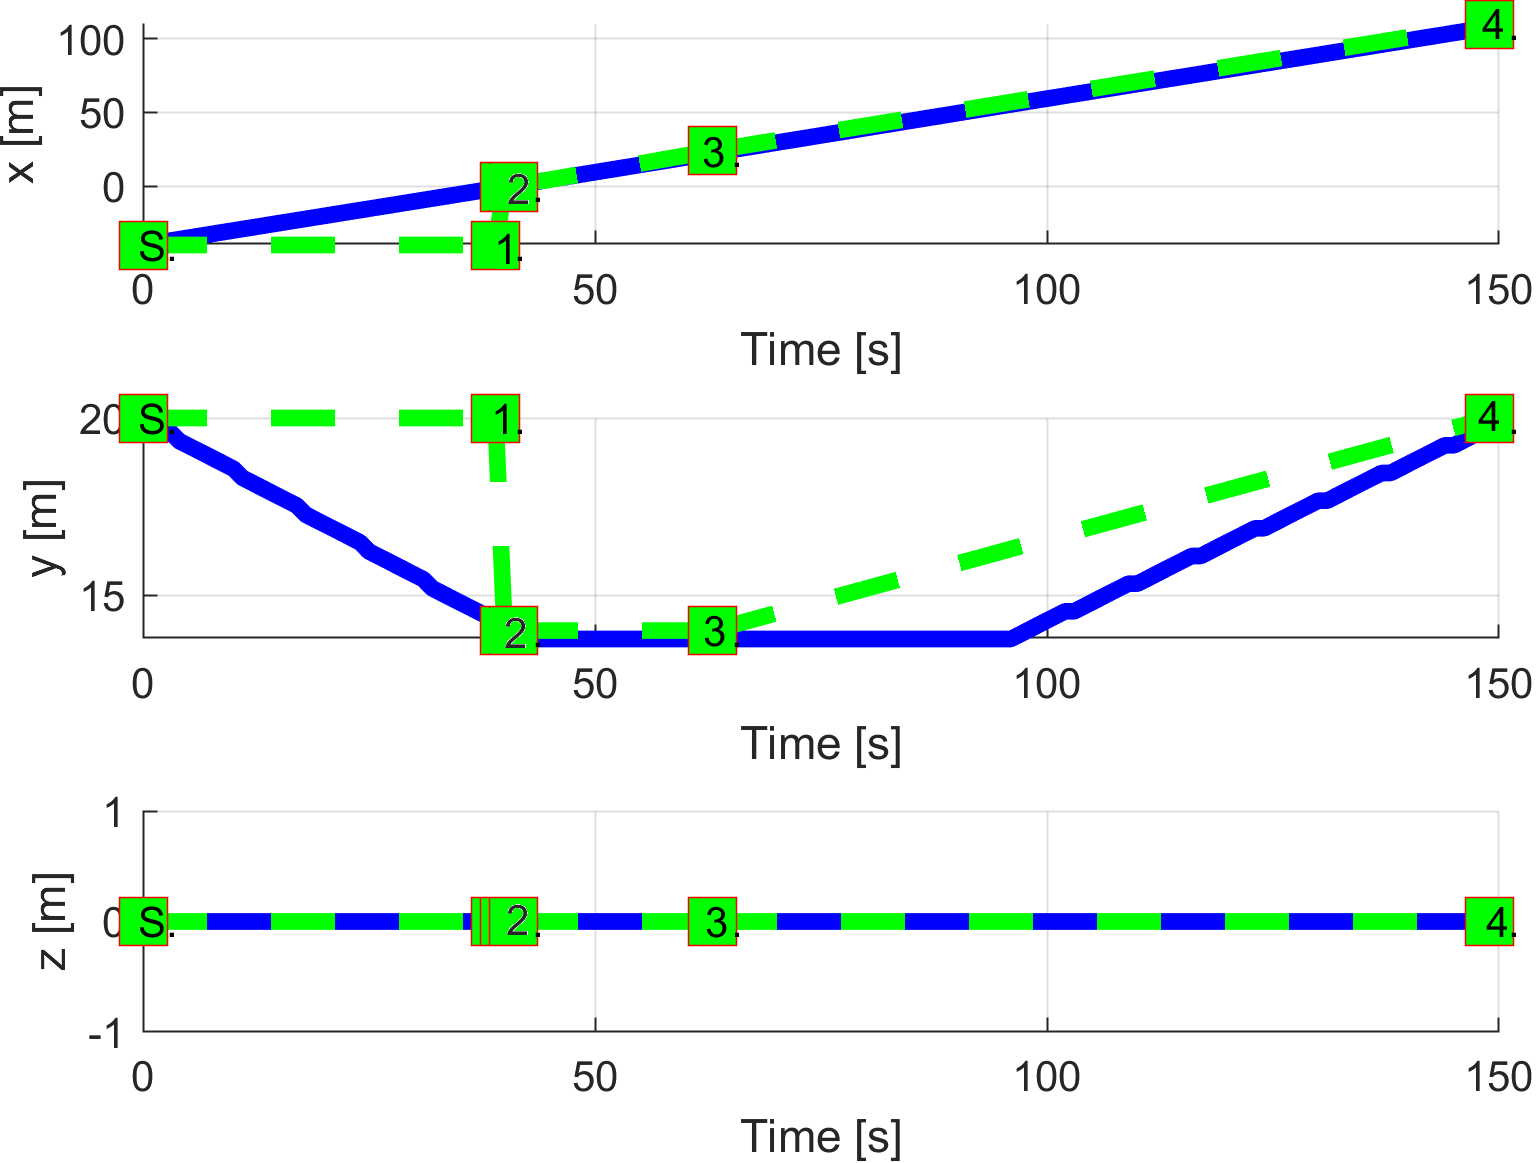
\includegraphics[width=0.9\linewidth]{\FIGDIR/NS076UtmCooperativeOvertake2xSpeedUAV1PathFollowing}
            \caption{UAS 1.}
            \label{fig:ruleBasedOvertake2xdPathTrackingUAS1}
        \end{subfigure}
        \begin{subfigure}{0.48\textwidth}
        	\centering
            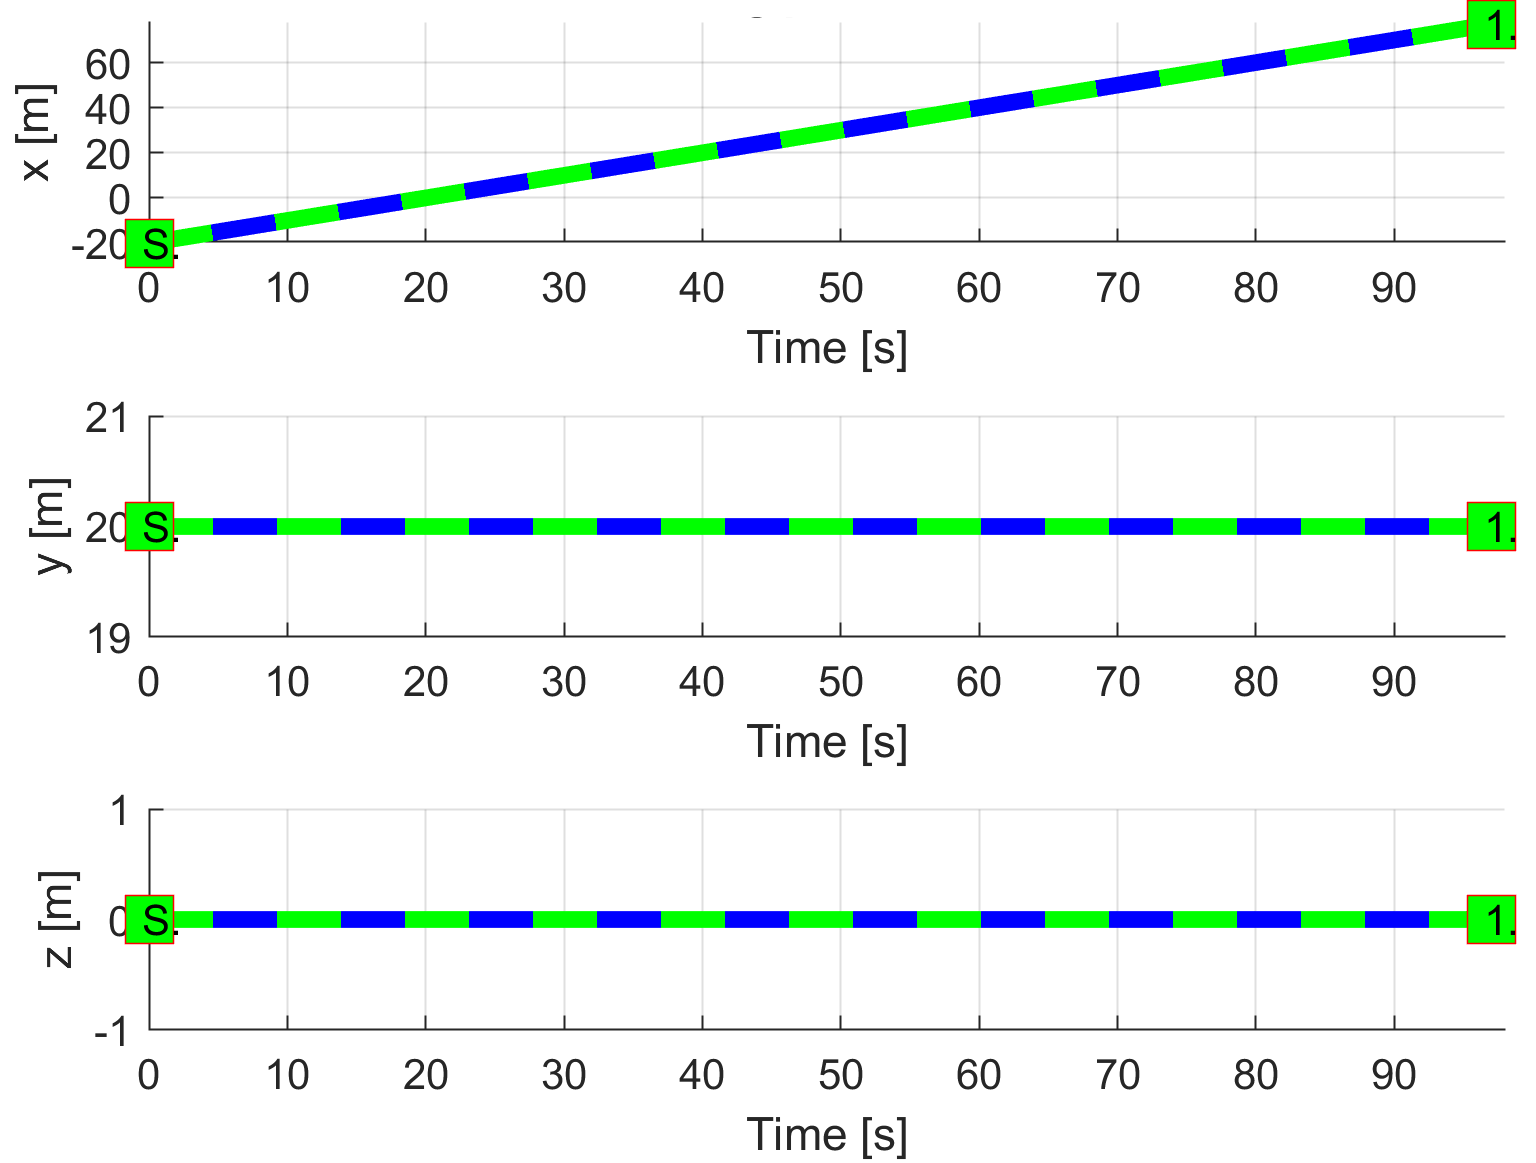
\includegraphics[width=0.9\linewidth]{\FIGDIR/NS077UtmCooperativeOvertake2xSpeedUAV2PathFollowing} 
            \caption{UAS 2.}
            \label{fig:ruleBasedOvertake2xPathTrackingUAS2}
        \end{subfigure}
        \caption{Trajectory tracking for \emph{Rule based overtake double speed} situation test case.}
        \label{fig:testCaseRuleBasedOvertake2xTrajectoryTracking}
    \end{figure}
    
	\newpage
    \paragraph{Path Tracking Deviations: 2x Speed} Path tracking deviations (tab. \ref{tab:pathTrackingParametersForRuleBasedOvertake2x}) are interesting for an \emph{Overtake Maneuver} performance. 
    
    \emph{Maximal deviation distance} is for important waypoints: Divergence ($\mathscr{WP}$ 2.), Convergence ($\mathscr{WP}$ 3.) and Original Goal Waypoint ($\mathscr{WP}$ 4.), equal to $0$ $m$. This is \emph{desired effect} for \emph{Overtake maneuver}.
    
    \emph{Collision point} ($\mathscr{WP}$ 1.) is avoided at minimal distance $5.7991$ $m$ (tab. \ref{tab:testCaseRuleBasedOvertakeSafetyMarginDistancesTimes}) and maximal distance $24.5$ $m$ (tab. \ref{tab:pathTrackingParametersForRuleBasedOvertake2x}). 
    
    Other \emph{Speed Difference Ratios} yields similar results.
    
    \begin{table}[H]
        \centering
        \begin{tabular}{c||c|c|c|c|c}
            \multirow{3}{*}{Param.} & \multicolumn{4}{c|} {UAS 1} & UAS 2     \\\cline{2-6}
                                    & $\mathscr{WP}_1$   & $\mathscr{WP}_2$ & $\mathscr{WP}_3$ & $\mathscr{WP}_4$ & $\mathscr{WP}_1$ \\\cline{2-6}
                                    & col.               & div.             & conv.            & orig.              & nav.              \\\hline\hline
              $\max |x|$            & 20                 & 0                & 0                & 0                & 0                \\\hline
              $\max |y|$            & 6                  & 0                & 4                & 5                & 0                \\\hline
              $\max |z|$            & 0                  & 0                & 0                & 0                & 0                \\\hline
              $\max dist.$          & 24.5                  & 0                & 4                & 5                & 0                \\
        \end{tabular}
        \caption{Path tracking properties for \emph{Rule overtake 2x speed} scenario.}
        \label{tab:pathTrackingParametersForRuleBasedOvertake2x}
    \end{table}


% 11 Rule Based Overtake
\paragraph{Computation Load:} The \emph{computation load} for \emph{scenario} (fig.\ref{fig:ruleBasedOvertakeComputationTime}) shows used time (y-axis) over decision frame (x-axis).

The load is minimal on both UAS, because the rule calculates only divergence (eq. \ref{eq:overtakedDivergenceGlobal}) and convergence (eq. \ref{eq:overtakeConvergenceGlobal}) waypoints.

\begin{figure}[H]
    \centering
    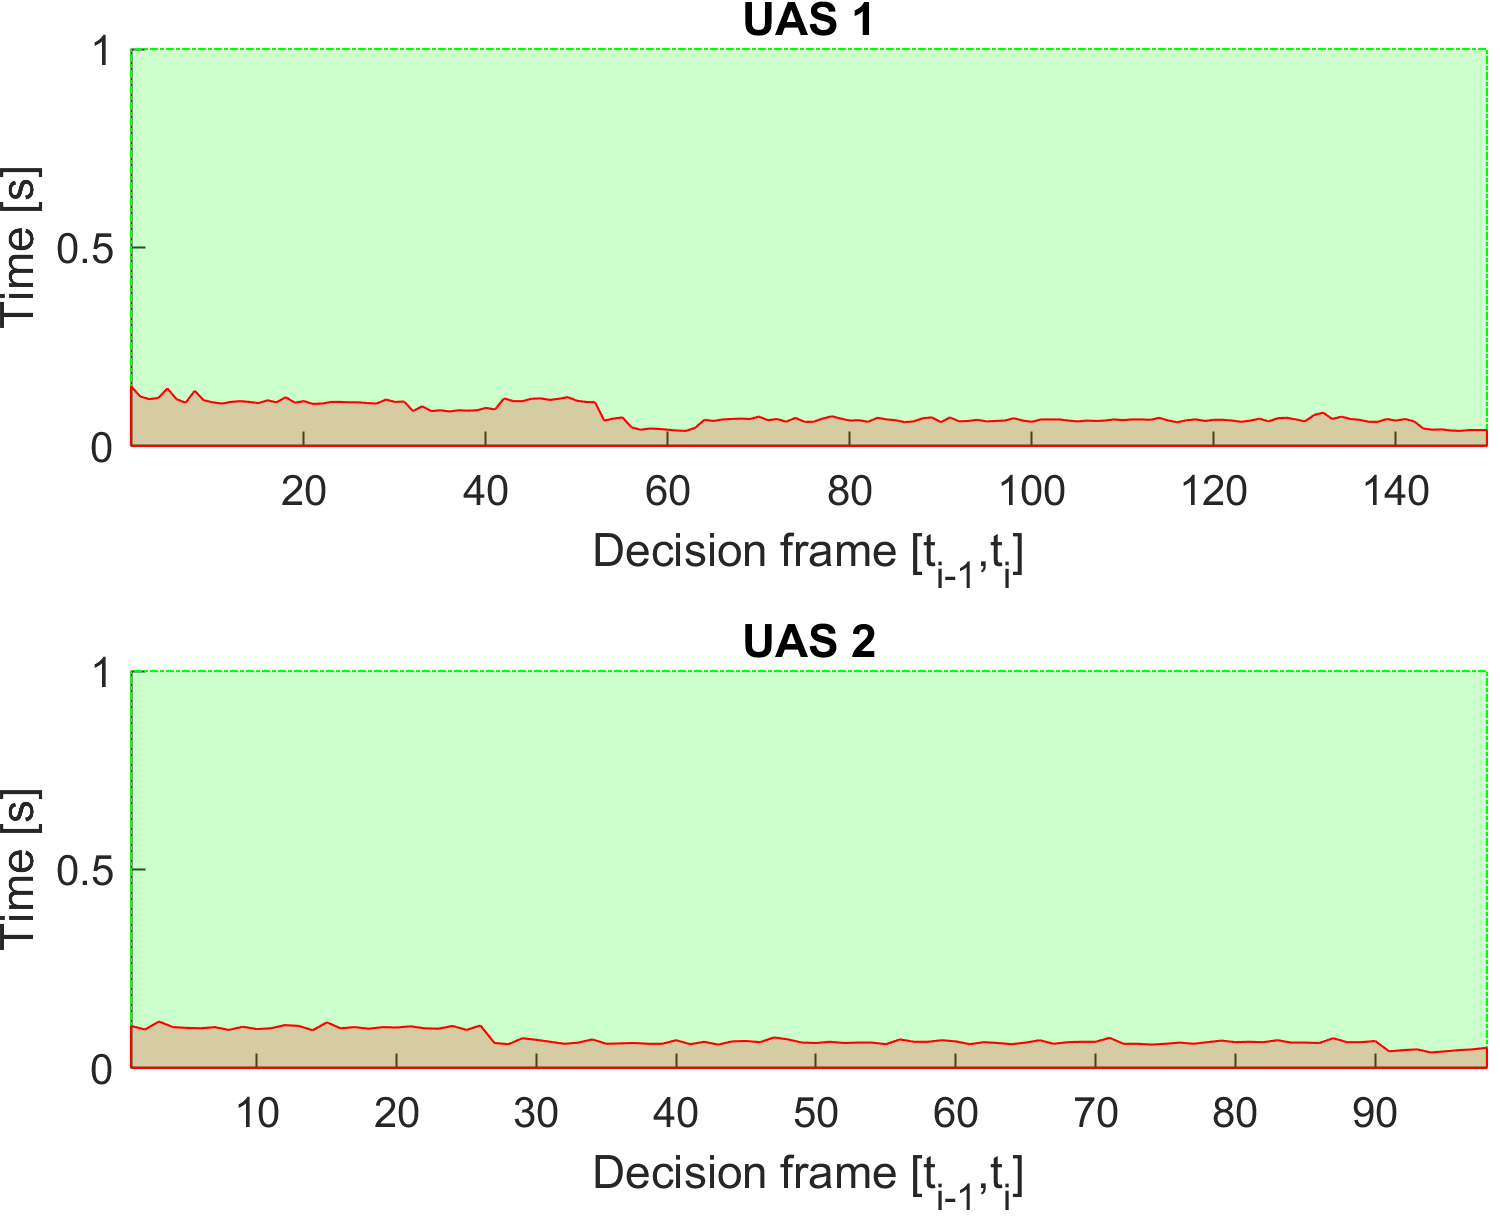
\includegraphics[width=0.65\linewidth]{\FIGDIR/NS102RuleBasedOvertakeComputationTime} 
    \caption{Computation time for \emph{Rule based overtake} scenario.}
    \label{fig:ruleBasedOvertakeComputationTime}
\end{figure}
	    	
    
%% This adds a line for the Bibliography in the Table of Contents.
\addcontentsline{toc}{chapter}{Bibliography}
%% *** Set the bibliography style. ***
%% (change according to your preference/requirements)
%\bibliographystyle{plain}
%% *** Set the bibliography file. ***
%% ("thesis.bib" by default; change as needed)
\bibliography{thesis}

%% *** NOTE ***
%% If you don't use bibliography files, comment out the previous line
%% and use \begin{thebibliography}...\end{thebibliography}.  (In that
%% case, you should probably put the bibliography in a separate file and
%% `\include' or `\input' it here).

\end{document}
